% Retoca las líneas marcadas con TODO según las necesidades

\documentclass[oneside,a4paper,12pt]{book} % TODO: cambia "oneside" por "twoside" a la hora de imprimirlo

\usepackage[spanish]{babel}
\usepackage[utf8]{inputenc}
\usepackage{geometry}
\usepackage{makeidx}
\usepackage{url}
\usepackage{graphicx}
\usepackage{color}
\usepackage{caption}
\usepackage{acronym}
\usepackage{hyphenat}
\usepackage{a4wide}
\usepackage[normalsize]{subfigure}
\usepackage{float}
\usepackage{titlesec}
\usepackage[Lenny]{fncychap}
\usepackage{listings} % para poder hacer uso de "listings" propios (p.ej. códigos)
\usepackage{eurosym} % para poder usar el símbolo del euro con \euro {xx}
\usepackage{hyperref} % TODO: añade la opción hidelinks para imprimirlo (los enlaces no aparecerán resaltados)

\usepackage{subfigure} 
% Para que no parta las palabras
\pretolerance=10000

\newcommand{\bigrule}{\titlerule[0.5mm]} \titleformat{\chapter}[display] % cambiamos el formato de los capítulos
{\bfseries\Huge} % por defecto se usaron caracteres de tamaño huge en negrita
{% contenido de la etiqueta 
\titlerule % línea horizontal 
\filright % texto alineado a la derecha 
\Large\chaptertitlename\ % capítulo e índice en tamaño large
\Large % en lugar de 
\Huge \Large\thechapter} 
{0mm} % espacio mínimo entre etiqueta y cuerpo
{\filright} % texto del cuerpo alineado a la derecha
[\vspace{0.5mm} \bigrule] % después del cuerpo, dejar espacio vertical y trazar línea horizontal gruesa
\geometry{a4paper, left=3.5cm, right=2cm, top=3cm, bottom=2cm, headsep=1.5cm}

% Estilos para ilustrar códigos:
\definecolor{code_green}{rgb}{0,0.6,0}
\definecolor{code_gray}{rgb}{0.5,0.5,0.5}
\definecolor{code_mauve}{rgb}{0.58,0,0.82}

\lstset{frame=tb,
  language=C,
  aboveskip=3mm,
  belowskip=3mm,
  showstringspaces=false,
  columns=flexible,
  basicstyle={\small\ttfamily},
  numbers=none,
  numberstyle=\tiny\color{code_gray},
  keywordstyle=\color{blue},
  commentstyle=\color{code_green},
  stringstyle=\color{code_mauve},
  breaklines=true,
  breakatwhitespace=true,
  tabsize=3
}

\lstset{frame=tb,
  language=C++,
  aboveskip=3mm,
  belowskip=3mm,
  showstringspaces=false,
  columns=flexible,
  basicstyle={\small\ttfamily},
  numbers=none,
  numberstyle=\tiny\color{code_gray},
  keywordstyle=\color{blue},
  commentstyle=\color{code_green},
  stringstyle=\color{code_mauve},
  breaklines=true,
  breakatwhitespace=true,
  tabsize=3
}

\lstset{frame=tb,
  language=Python,
  aboveskip=3mm,
  belowskip=3mm,
  showstringspaces=false,
  columns=flexible,
  basicstyle={\small\ttfamily},
  numbers=none,
  numberstyle=\tiny\color{code_gray},
  keywordstyle=\color{blue},
  commentstyle=\color{code_green},
  stringstyle=\color{code_mauve},
  breaklines=true,
  breakatwhitespace=true,
  tabsize=3
}

% Definición de mis propios tipos: Códigos, Ecuaciones y Tablas
\DeclareCaptionType{code}[Código][Listado de códigos]
\DeclareCaptionType{myequation}[Ecuación][Listado de ecuaciones]

% TODO: especifica las reglas de separación que consideres. Algunos ejemplos:
\hyphenation{fuer-tes}
\hyphenation{mul-ti-ca-pa}
\hyphenation{res-pues-ta}
\hyphenation{di-fe-ren-tes}
\hyphenation{de-sa-rro-lla-dos}
\hyphenation{re-pre-sen-tan-do}

 % archivo de configuraci�n de estilo

\makeindex

\begin{document}
\baselineskip 1.35\baselineskip

\frontmatter

\thispagestyle{empty}
\vspace{2cm}

\begin{figure}[htb]
  \centerline{\resizebox{.60\textwidth}{!}{
\includegraphics{figs/logo_urjc}}}
\end{figure}

\begin{center}
  {\Large {\bf GRADO EN INGENIERÍA DE ROBÓTICA SOFTWARE}}
  \vspace{5mm}
 
  {\large {Escuela Técnica Superior de Ingeniería de Telecomunicación}}
  \vspace{5mm}

  {\large {Curso académico 2021-2022}}

  \vspace{1cm}

  {\large {\bf Trabajo fin de grado}}

  \vspace{2cm}

  {\Large {Sistema de Monitorización de animales de laboratorio\\
               bajo plataforma de bajo coste\\[1cm] }}

  \vspace{5cm}
  {\bf Tutor}: Julio Vega Pérez \\
  {\bf Autor}: Isabel Cebollada Gracia
\end{center}

\clearpage
\thispagestyle{empty}


% Este diseño se corresponde con la licencia CC-BY-NC-SA.
% Por supuesto, puedes poner la licencia que mejor se adapte al propósito de tu trabajo.
% Recuerda que, si no se especifica ninguna licencia, esta -como cualquier creación artística- pasaría a estar licenciada con todos los derechos reservados (copyright).

\cleardoublepage

\begin{figure}
 \ \ \ \ 
\includegraphics[width=0.25\linewidth]{figs/by-nc-sa.png}
 \label{fig:cc} 
 \end{figure}

\

\

\

\noindent
Este trabajo se distribuye bajo los términos de la licencia internacional \href{http://creativecommons.org/licenses/by-nc-sa/4.0/}{CC BY-NC-SA International License} (Creative Commons AttributionNonCommercial-ShareAlike 4.0). Usted es libre de \textit{(a) compartir}: copiar y redistribuir el material en cualquier medio o formato; y \textit{(b) adaptar}: remezclar, transformar y crear a partir del material. El licenciador no puede revocar estas libertades mientras cumpla con los términos de la licencia:

\begin{itemize}
\item \textit{Atribución}. Usted debe dar crédito de manera adecuada, brindar un enlace a la licencia, e indicar si se han realizado cambios. Puede hacerlo en cualquier forma razonable, pero no de forma tal que sugiera que usted o su uso tienen el apoyo de la licenciante.
\item \textit{No comercial}. Usted no puede hacer uso del material con propósitos comerciales.
\item \textit{Compartir igual}. Si remezcla, transforma o crea a partir del material, debe distribuir su contribución bajo la la misma licencia del original.
\end{itemize}

\begin{flushright}
		\vspace{7.0 cm}
		\emph{Documento de} \textbf{Isabel Cebollada}. % TODO: pon aquí tu nombre cuando hagas el documento
\end{flushright}



\cleardoublepage

\chapter*{Agradecimientos}

Unas bonitas palabras...\\

Quizás un segundo párrafo esté bien. No te olvides de nadie.\\

Un tercero tampoco viene mal para contar alguna anécdota...\\

¿Alguien más? Aunque sean \textit{actores} secundarios.\\

Un quinto párrafo como colofón.\\
\ % Algo de separación...

\

\

\

\

\begin{flushright}
		\vspace{4.0 cm}
		\emph{A alguien especial;\\
      si no, tampoco pasa nada}\\
		\par
		\vspace{1.0 cm}
		Madrid, xx de xxxxxx de 20xx\\ %\today
		\emph{Tu nombre}
\end{flushright}

\thispagestyle{empty}



\cleardoublepage

\chapter*{Resumen\markboth{Resumen}{Resumen}}
Gracias al desarrollo tecnológico, la robótica está adquiriendo cada vez más importancia en diferentes campos, facilitando y simplificando el trabajo de las personas debido a la eficiencia y automatización de sistemas previamente manejados por humanos.\\

Uno de los campos claves en robótica es la inteligencia artificial, que pretende replicar el funcionamiento del cerebro humano. A su vez, uno de sus campos más importantes es la visión artificial, que pretende imitar el funcionamiento de la visión humana. Para ello, es importante el entrenamiento de algoritmos. Los más usados son algoritmos de Deep Learning, que tratan de replicar la estructura de las neuronas.\\

Para este TFG se ha creado un sistema de monitorización para el control y estudio del bienestar de ratones. Se ha contactado con los investigadores del Laboratorio de Bienestar e Investigación Animal de la UAH para el conocimiento de los requisitos reales, los cuales se han analizado y se les ha dado solución mediante el desarrollo de una interfaz de usuario que ofrece de forma simple los datos recopilados por el sistema.\\

Para la implementación de este sistema, se ha utilizado la placa Raspberry Pi 4, lo que permite que el sistema sea \textit{low-cost}. La interfaz se ha creado en Node-Red, donde se han recogido las lecturas de los distintos sensores así como los servidores web de las cámaras, creados con Flask. Además se ha creado un dataset con imágenes de ratones, que ha permitido entrenar un modelo de detección en YOLO, entrenado a través de una red neuronal convolucional, un tipo de algoritmo de Deep Learning.\\

El resultado ha sido una interfaz de usuario amigable para el usuario. A pesar de ello, existen mejoras que podrían aplicarse en un futuro al sistema desarrollado como el uso de un Docker para la instalación rápida y sencilla por cualquier usuario, el análisis del comportamiento de los animales con Deep Learning o el acceso de la interfaz de usuario desde cualquier lugar.

\cleardoublepage

\chapter*{Acrónimos\markboth{Acrónimos}{Acrónimos}}

% Añade a continuación los acrónimos que uses en el documento. Algunos ejemplos:
\begin{acronym}
	\acro{IA}{\emph{Inteligencia Artificial}}
	\acro{VA}{\emph{Visión Artificial}}
	\acro{ML}{\emph{Machine Learning}}
	\acro{IU}{\emph{Interfaz de Usuario}}
\end{acronym}


\cleardoublepage

\tableofcontents

\listoffigures

\listofcodes

\listofmyequations

\listoftables

\pagestyle{empty}

\cleardoublepage

 % aqu� se cargan todas las "primeras p�ginas"

% Bibliograf�a
\let\OLDthebibliography=\thebibliography
\def\thebibliography#1{\OLDthebibliography{#1}
  \addcontentsline{toc}{chapter}{\bibname}}

\mainmatter

\chapter{Introducción}
\label{cap:capitulo1}
\setcounter{page}{1}

\begin{flushright}
\begin{minipage}[]{10cm}
%\emph{Quizás algún fragmento de libro inspirador...}\\
\end{minipage}\\

%Autor, \textit{Título}\\
\end{flushright}

\vspace{1cm}

El desarrollo tecnológico ha provocado el avance en la robótica, un campo de investigación muy amplio en la actualidad que está facilitando la vida a los humanos. Cualquier robot está formado por tres componentes principales: un sistema de control, sensores y actuadores. Dentro de los numerosos sensores que pueden tener los robots, uno de los que está adquiriendo mayor relevancia en los últimos años es el sensor de visión.\\

Los sensores de visión aportan mucha información y son baratos, pero se requiere de un proceso arduo para extraer la información útil en tiempo real. Por este motivo se busca la eficiencia en resultados y tiempo, lo que significa el proceso de la extracción de la información debe ser rápido. Es por ello que en los últimos años, en el campo de la visión artificial moderna, están adquiriendo gran importancia los algoritmos de Deep Learning (DL) o aprendizaje profundo.\\

Los algoritmos más utilizados hoy en día para obtener la información de los sensores de Visión Artificial (VA) se obtienen bajo la técnica del Machine Learning (ML) o aprendizaje automático. Estos algoritmos son mejores que los que se tenían anteriormente, y se han podido desarrollar gracias al avance de la capacidad de cómputo. El objetivo del ML es que las máquinas sean capaces de aprender sin tener que ser programadas explícitamente.\\

Un subcampo del ML es el DL, que aunque utiliza algoritmos de ML, sus algoritmos se basan en estructuras similares al modelo del cerebro humano, emulando redes neuronales. Según el algoritmo de DL obtiene más información, aumenta su precisión. Debido a su gran capacidad de abstracción, es el más usado en VA.\\

A continuación se describen estos conceptos y el contexto en el que se enmarca el presente trabajo. Asimismo se presentan sistemas actuales que existen en el mercado con una idea similar a la de este trabajo.\\

\section{La robótica}
\label{sec:robotica}
La robótica, aunque no siempre bajo ese nombre, se lleva utilizando desde hace mucho tiempo con el propósito de desarrollar herramientas automatizadas.
Hasta mediados del siglo pasado, esta disciplina se centraba en el desarrollo de máquinas que realizaban un trabajo que resultaba tedioso, debido a su repetitividad, para el ser humano. Esta concepción se refleja con Henry Ford y la producción en serie de su fábrica de coches inaugurada en 1901 (Figura \ref{fig:ford}).\\
\begin{figure} [h!]
  \begin{center}
    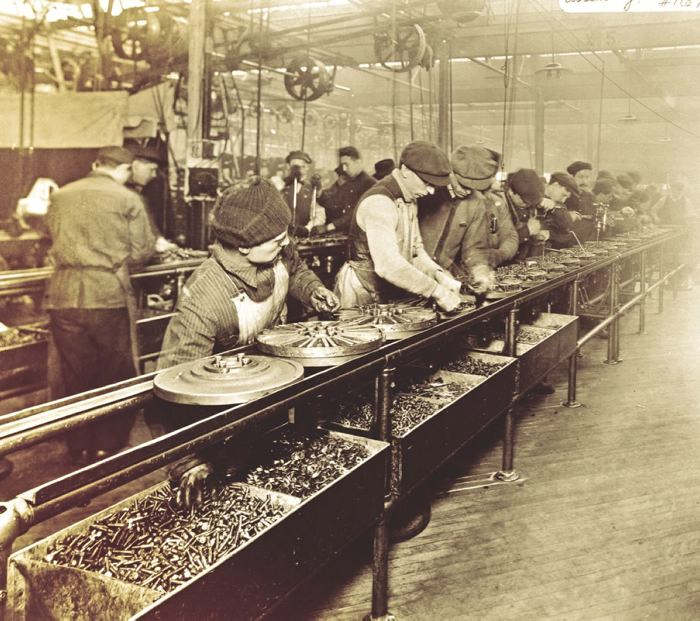
\includegraphics[width=8cm]{figs/ford}
  \end{center}
  \caption{Producción en serie en la fábrica de coches Ford.}
  \label{fig:ford}
\end{figure}

Sin embargo, la palabra \textit{robota} ---origen de la palabra robot que significa trabajo forzado--- aparece por primera vez en 1921 en una obra de teatro de un autor checo llamado Karel Capek. Empezando a concebir esta palabra a principios de siglo pasado, comenzó a nacer el desarrollo de la idea de robótica que existe hoy en día y que no se centra exclusivamente en el desarrollo de herramientas automatizadas, sino que se concibe como una industria interdisciplinaria que surge de la intersección de la ciencia, la ingeniería y la tecnología. Esta nueva concepción une el conocimiento científico, computacional e informático con diversas ramas de la ingeniería, ya que no solo implica el estudio de robots, sino también de su diseño, programación y aplicación. Así, la robótica incluye disciplinas como la IA, la informática, la VA, la programación o el álgebra, entre otras muchas.\\

Tras la primera aparición de la palabra \textit{robota}, la definición de robot ha ido formándose hasta la que hay en la actualidad:  cualquier máquina que opera de forma automática y autónoma, y que sustituye a los seres humanos en determinadas tareas, especialmente las peligrosas, aburridas o pesadas. Está compuesto por el sistema de control, los sensores y los actuadores.\\

La analogía de un robot respecto a un ser humano es la siguiente. Los sensores son sus sentidos, que transmiten la información percibida, bien sea del propio robot o del entorno al sistema de control, que se asemeja al cerebro humano. El sistema de control toma decisiones adaptándose a la información recibida, que modifica bien el entorno o bien la manera de actuar internamente del propio robot. Y finalmente los actuadores, que permiten la modificación del entorno; su equivalente en el cuerpo humano serían las extremidades.\\

El objetivo de la robótica es ayudar al ser humano en todos los ámbitos, tanto en la vida cotidiana como en la vida profesional, evitando los trabajos perjudiciales, e incluso haciendo trabajos que el ser humano no sería capaz de hacer por sí mismo en distintos sectores.\\

Uno de estos sectores es la medicina. En este ámbito cabe resaltar el robot Da Vinci (Figura \ref{fig:da-vinci}), uno de sus robots más famosos que permite a un cirujano comandar órdenes a través de una consola, permitiéndole realizar cirugías de alta precisión eliminando los temblores nerviosos que un humano pueda tener y permitiendo al cirujano una mayor visión. Otro ejemplo se encuentra en el campo de la medicina se encuentra en la impresión 3D. En \cite{ANDRESCANO2021138}, la impresión 3D de biomodelos de partes del cuerpo como huesos adquiere un papel útil en fracturas complejas, displasias de cadera o en tumores óseos principalmente. Con estos biomodelos, no solo disminuye tanto el tiempo quirúrgico como los costes de intervención, sino que además se reduce la dosis intraoperatoria de radiación. También sirven para la planificación preoperatoria (Figura \ref{fig:3d}-a) o el premodelado de placas (Figura \ref{fig:3d}-b). Con la impresión 3D también se han creado férulas para los pacientes (Figura \ref{fig:3d}-c). Ofrecen una mayor adaptación a la anatomía del paciente que las férulas de yeso o plástico que se acostumbran a llevar.\\
\begin{figure} [h!]
  \begin{center}
    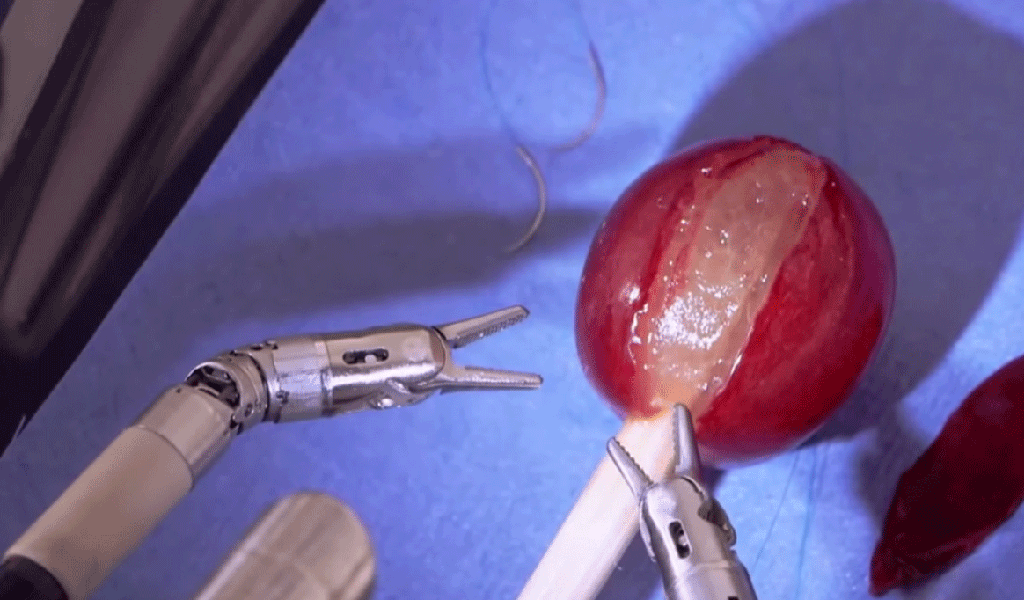
\includegraphics[width=8cm]{figs/da-vinci}
  \end{center}
  \caption{Robot Da Vinci}
  \label{fig:da-vinci}
\end{figure}

\begin{figure}[h!]
  \begin{center}
    \subfigure[Preoperatoria]{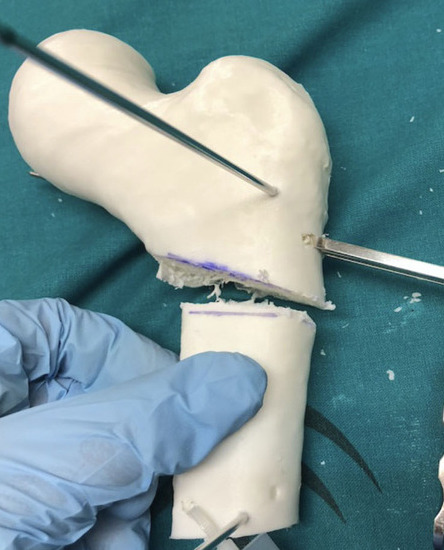
\includegraphics[width=41mm]{figs/preop}}\hspace{2mm}
    \subfigure[Premodelado de placas]{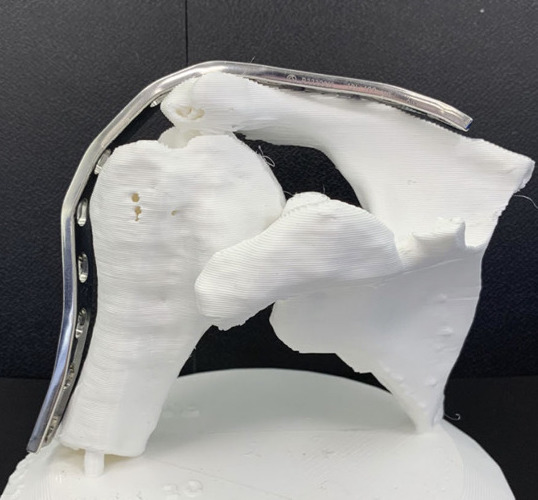
\includegraphics[width=55mm]{figs/premodelado}}
    \subfigure[Férulas con impresión 3D]{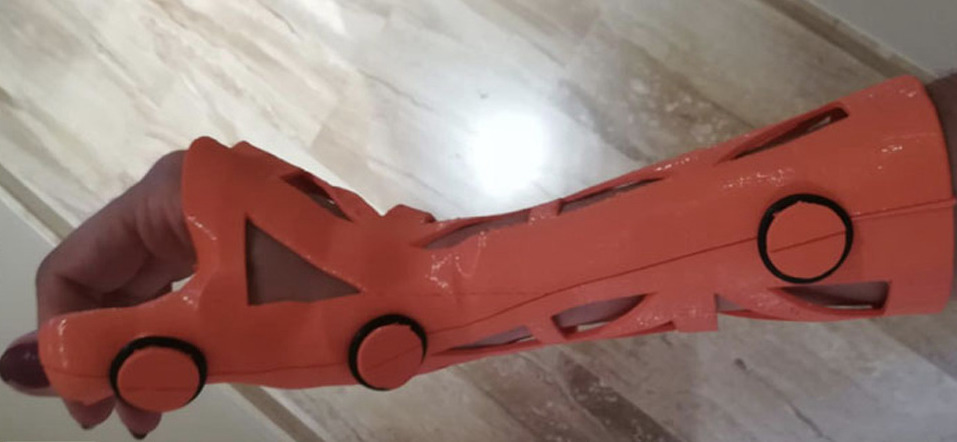
\includegraphics[width=100mm]{figs/ferula}}
  \end{center}
\caption{Usos de la impresión 3D en medicina.} \label{fig:3d}
\end{figure}

Otro de los campos más importantes de la robótica es la manipulación en entornos inaccesibles u hostiles por el ser humano. Un ejemplo de ello lo encontramos en la carrera espacial. Uno de estos robots es el Curiosity (Figura \ref{fig:robots}-a), cuya misión era evaluar la habitabilidad en Marte recogiendo información del entorno. Otro ejemplo de entornos hostiles se encuentra en el lugar que quedó tras el accidente nuclear que ocurrió en Fukushima en 2011, causado por un terremoto y el consecuente tsunami. Gracias a los robots (Figura \ref{fig:robots}-b) se pudo acceder a la zona para poder limpiarla.\\
\begin{figure}[h!]
  \begin{center}
    \subfigure[Robot Curiosity]{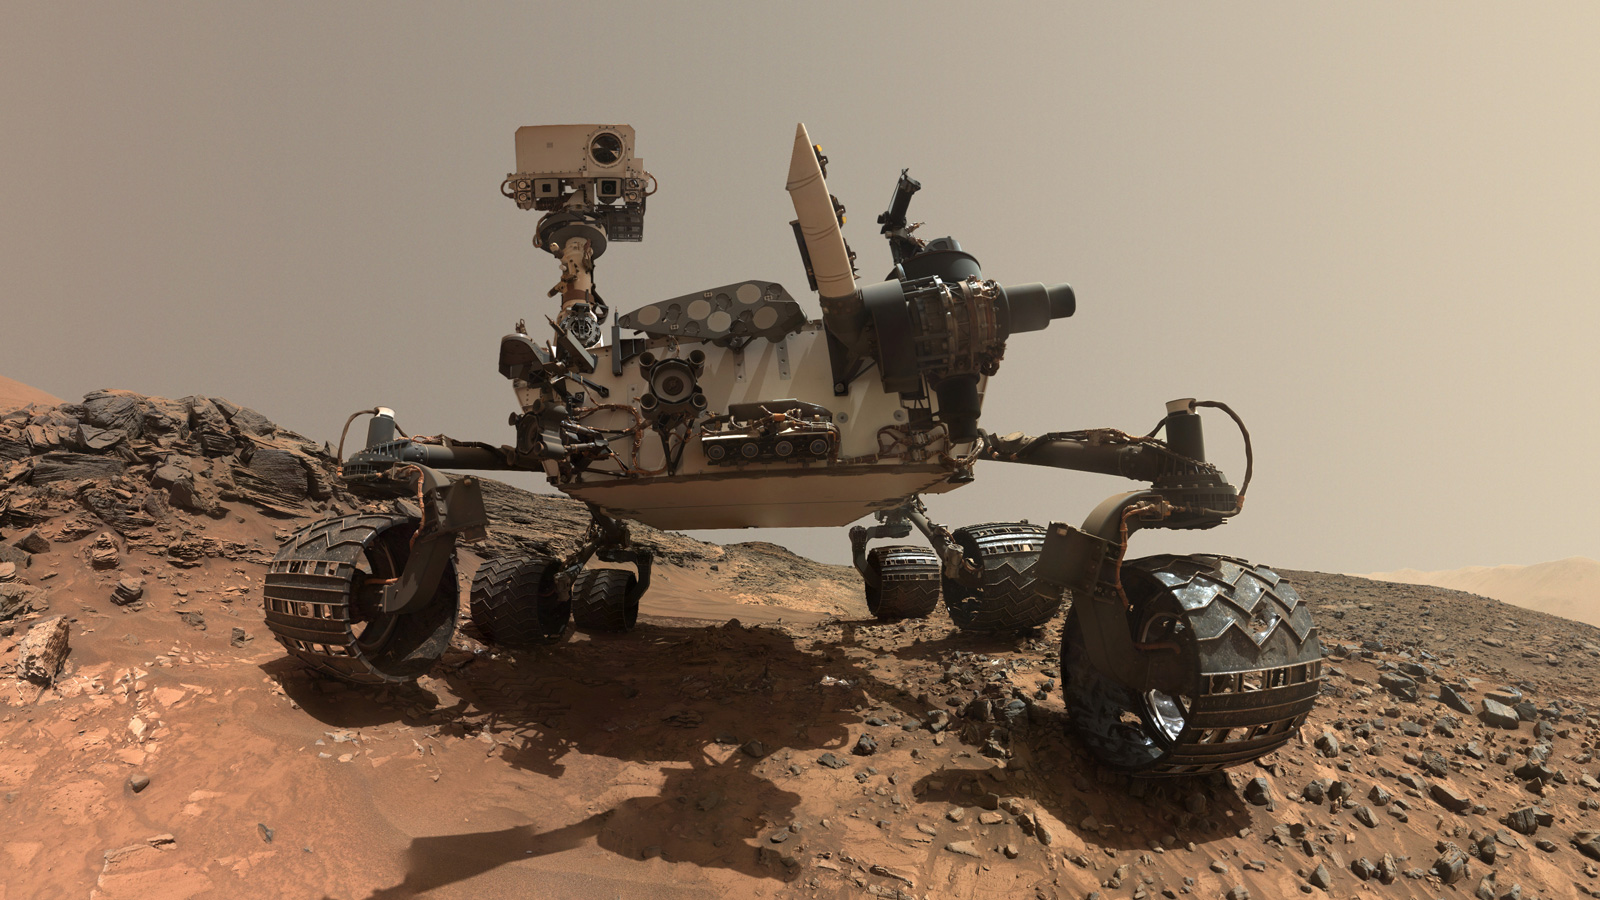
\includegraphics[width=82mm]{figs/curiosity}}\hspace{2mm}
    \subfigure[Robot en Fukushima]{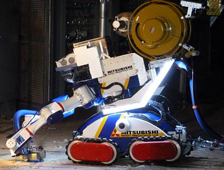
\includegraphics[width=61mm]{figs/fukushima}}
  \end{center}
\caption{Ejemplos de la robótica en diferentes campos.} \label{fig:robots}
\end{figure}

La industria del automóvil, con los coches autónomos (Figura \ref{fig:coches}-a), es otro de los grandes frentes de la robótica. El objetivo es que un coche sea capaz de realizar todas las tareas de conducción de forma autónoma. Como medio autónomo, es capaz de percibir el medio que le rodea y navegar en consecuencia.
\begin{figure}[h!]
  \begin{center}
    \subfigure[Coche autónomo de Google]{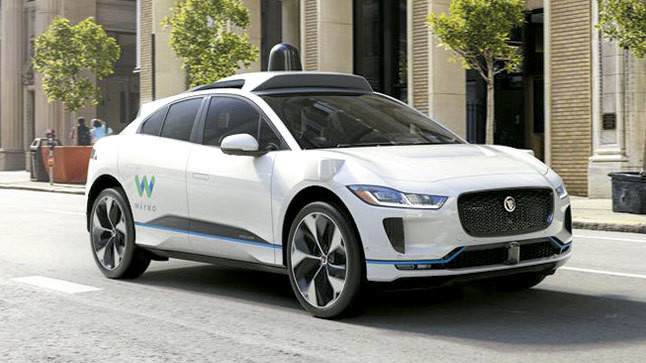
\includegraphics[width=7.5cm]{figs/coche}}
    \subfigure[Vision de un Tesla autónomo]{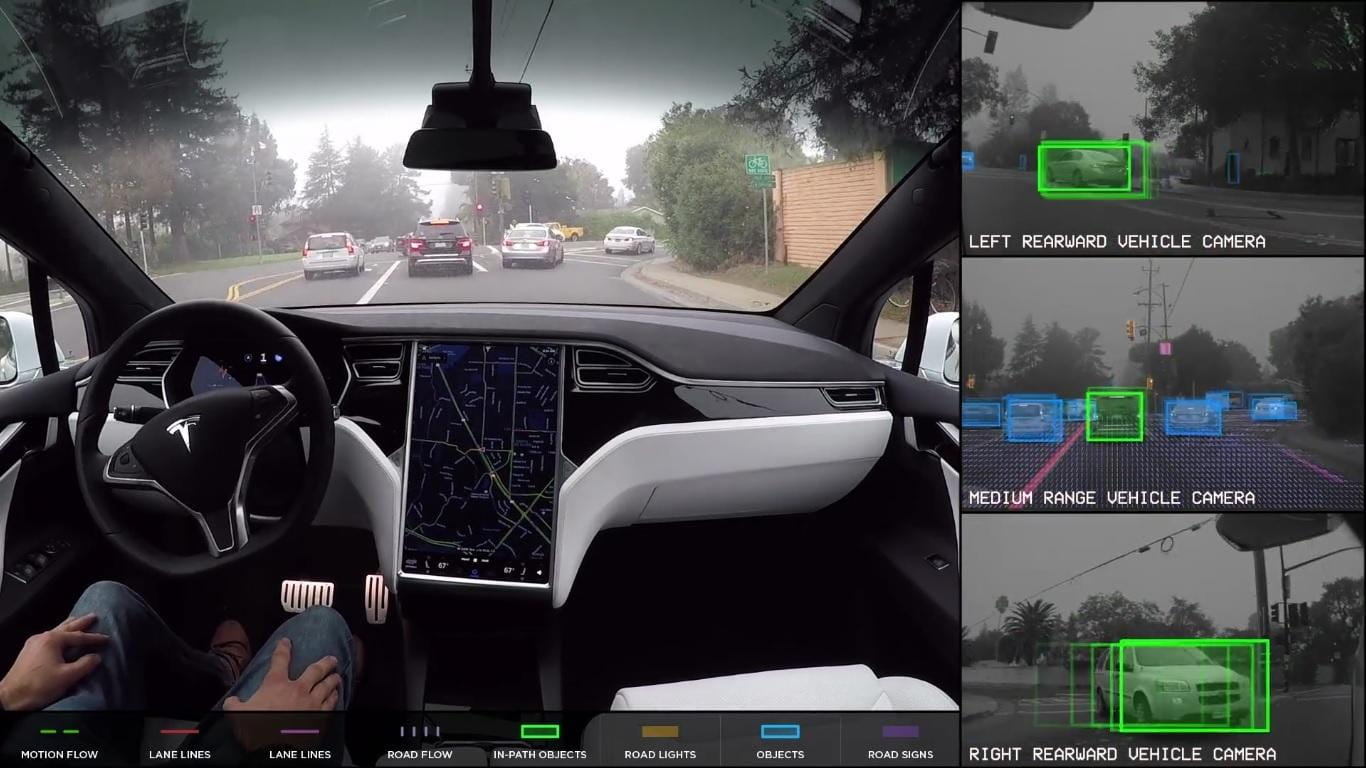
\includegraphics[width=7.5cm]{figs/coche_autonomo}}
  \end{center}
\caption{Ejemplos de la robótica en diferentes campos.} \label{fig:coches}
\end{figure}

\section{Inteligencia Artificial}
La robótica engloba un conjunto de diferentes disciplinas que permiten abordar todos los campos que esta comprende. Uno de los campos más importantes es la Inteligencia Artificial (IA), que consiste en replicar los mecanismos del cerebro humano mediante algoritmos que emplean unidades equivalentes a las neuronas. Estos algoritmos van aprendiendo a medida que realizan sus tareas en base a la experiencia que van adquiriendo durante su ejecución.\\

Numerosos son los estudios existentes en la actualidad sobre la IA. Uno de ellos es la mejora del rendimiento y la eficiencia  del reconocimiento de fracturas radiográficas a través de la IA \cite{guermazi21}. Este algoritmo es capaz de detectar las fracturas en las radiografías con un menor rango de fallo y en menor tiempo que un humano. En el caso de la Figura \ref{fig:rad1}, nueve especialistas no detectaron la fractura mientras que el algoritmo sí.\\
\begin{figure} [h!]
  \begin{center}
    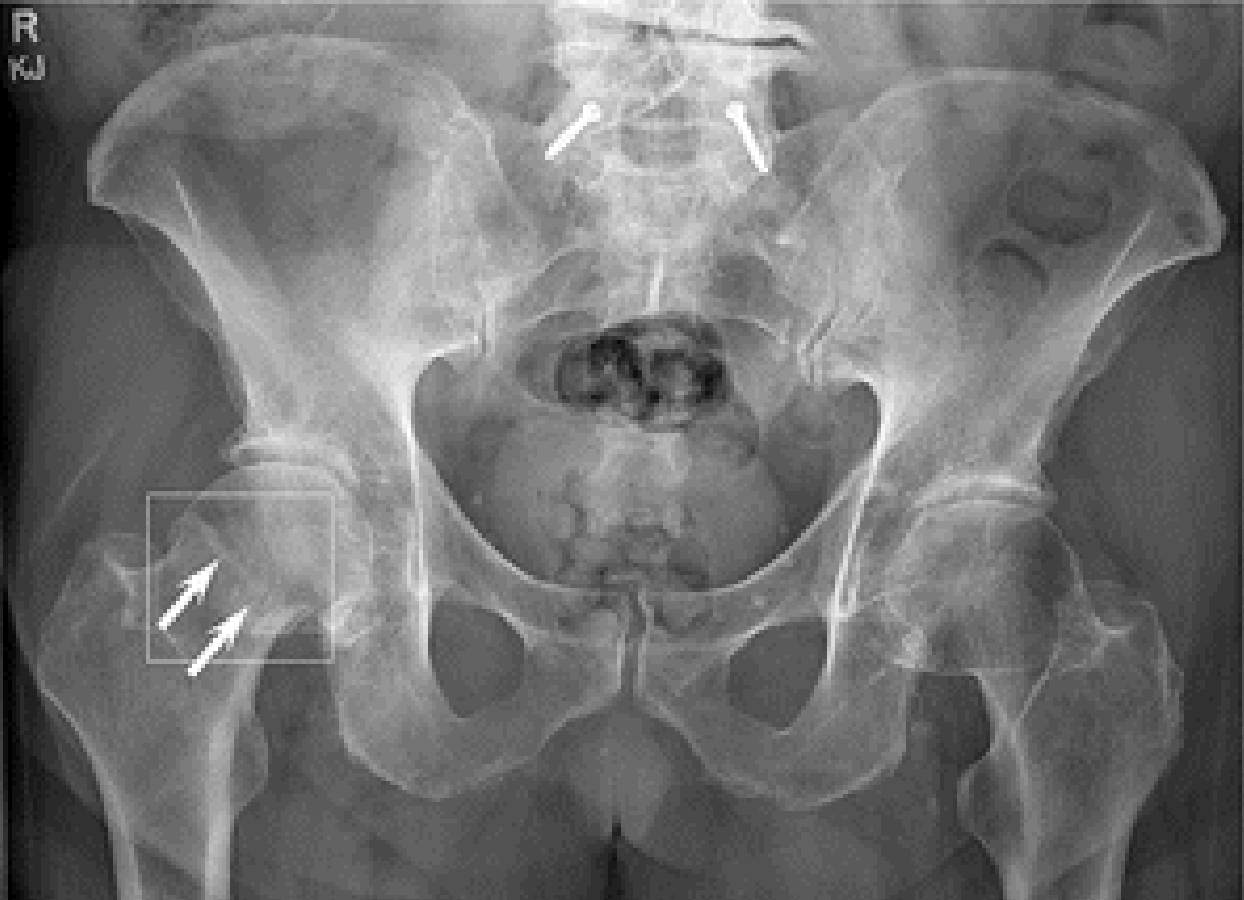
\includegraphics[width=8cm]{figs/rad1}
  \end{center}
  \caption{Detección de fracturas en la radiografía mediante IA}
  \label{fig:rad1}
\end{figure}

Hay dos tipos de inteligencia artificial:
\begin{itemize}
 \item{IA fuerte,} compuesta por la IA general y la superinteligencia artificial. La IA general está inspirada en la teoría de que una máquina adquiera inteligencia humana, siendo capaz de resolver cualquier problema por sí misma. Por otro lado, la superinteligencia artificial supera la capacidad del cerebro humano. La IA fuerte es todavía teórica y no hay ejemplos reales de su uso.
  \item{IA débil,} entrenada para realizar tareas específicas que operan dentro de un rango previamente definido. Los sistemas dotados con esta inteligencia parecen inteligentes, pero están limitados al contexto en el que trabajan. Un ejemplo de ello es el asistente de voz Siri de Apple.
\end{itemize}

La IA abarca diferentes áreas, como la comprensión, el reconocimiento o el aprendizaje. Una de las líneas de investigación dentro de la IA es la VA, que se detalla a continuación.\\

\subsection{Visión Artificial}
\label{sec:subseccion}
La visión artificial es uno de los campos más importantes de la IA cuyo objetivo es que un sistema inteligente obtenga la información en tiempo real más relevante de las imágenes que percibe. Así como la IA trata de emular un cerebro humano, la VA hace lo mismo con respecto a la visión humana, con la diferencia de que esta segunda cuenta con las experiencias aprendidas para, entre otras cosas, diferenciar los elementos que le rodean, su movimiento, distancia o tamaño. Así pues, la visión artificial trata de asemejar el funcionamiento del ojo humano y su posterior procesamiento con el cerebro mediante  una cámara y el posterior procesamiento de los datos que esta vierte.\\

Tiene diferentes usos, entre ellos los más fundamentales son:
\begin{itemize}
 \item \textit{Clasificación de imágenes (Figura \ref{fig:vision}-a).} Consiste en asignar imágenes a una serie de categorías predefinidas a través de un algoritmo. Es necesario contar con una gran cantidad de datos para poder tener suficiente entrenamiento y así fallar lo mínimo posible.
 \item \textit{Detección de objetos (Figura \ref{fig:vision}-b).} Consiste en analizar partes de la imagen para localizar objetos señalándolos mediante cuadros limitadores. Esto se consigue mediante el entrenamiento de una gran cantidad de imágenes en las que se etiquetan diferentes tipos de objetos, obteniendo así los datos que se usarán para la detección en una imagen.
  \item \textit{Segmentación de imágenes(Figura \ref{fig:vision}-c).} Consiste en el enmascaramiento exacto de los píxeles que representan a los objetos en una imagen. Es un paso más en la detección de objetos, siendo capaz de separar el objeto concreto del resto de la imagen. 
\end{itemize}
\begin{figure}[h!]
  \begin{center}
    \subfigure[Clasificación]{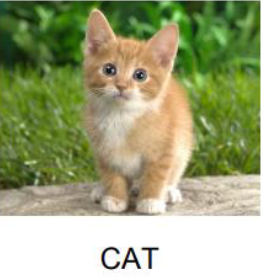
\includegraphics[width=43mm]{figs/clasificacion}}\hspace{8mm}
    \subfigure[Detección]{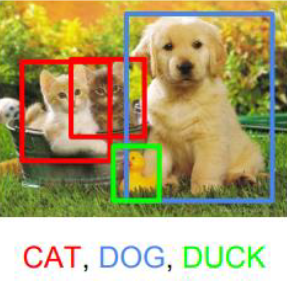
\includegraphics[width=45mm]{figs/deteccion}}\hspace{8mm}
    \subfigure[Segmentación]{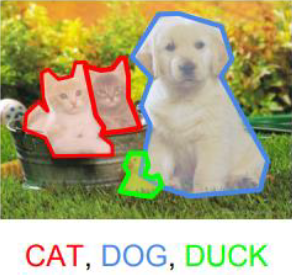
\includegraphics[width=47mm]{figs/segmentacion}}
  \end{center}
\caption{Algunos usos en la visión artificial.} \label{fig:vision}
\end{figure}

Un sistema dotado de visión funciona siguiendo tres niveles de operación. En primer lugar, la obtención de imágenes o vídeos mediante una cámara, las cuales son transferidas al sistema. En segundo lugar, el procesamiento de estas imágenes para poder representar correctamente los datos de interés. Este proceso consiste en un trabajo automático del sistema en el que se elimina el ruido, se reescalan las imágenes o se ajusta el contraste, entre otros, para adaptar las imágenes. Finalmente, se realiza la comprensión de imágenes, que es el paso clave para que el sistema pueda llamarse inteligente, donde a través de un modelo de aprendizaje, es capaz de llevar a cabo su propósito, como puede ser detectar un determinado objeto utilizando datos aprendidos en el pasado.\\

Un ejemplo muy extendido de uso de la VA son los coches autónomos (Figura \ref{fig:coches}-b). En este caso, el funcionamiento de la VA ha de ser impecable debido a las graves consecuencias que supondría el más mínimo fallo. Con el uso de cámaras y sensores, el ordenador del coche es capaz de detectar los objetos de las imágenes que recibe, como señales o semáforos ---entre otros--- y actuar en consecuencia según el estado de estos. Así, el coche es capaz de tener una vista de 360º y de reconocer todos los elementos de su entorno para ser capaz de actuar como lo haría un humano.\\

Para que la VA funcione correctamente es necesario disponer de algoritmos precisos que sean fiables. Entre los distintos métodos que existen para entrenar estos algoritmos, uno de los más utilizados es el ML, que se detalla a continuación.

\section{Machine Learning}
Para que la IA pueda simular al cerebro humano, debe ser capaz también de aprender. Este aprendizaje se lleva a cabo a través de algoritmos. Dentro de la IA se encuentra una categoría denominada Machine Learning o aprendizaje automático, cuyo fin es que los algoritmos descubran patrones en conjuntos de datos que les hacen aprender y mejorar respecto a la experiencia anterior pudiendo así tener un aprendizaje autónomo para poder realizar una tarea sin ayuda externa.\\

En el sistema de aprendizaje de un algoritmo de ML hay tres partes principales. En primer lugar, un proceso de decisión, en el que una vez recibidos los datos de entrada el algoritmo genera una estimación en los datos partiendo de un patrón. Los datos de entrada pueden estar o no etiquetados; si lo están, indican al modelo lo que debe identificar. La segunda parte es una función de error, que sirve para evaluar la precisión del modelo sobre la decisión tomada. La tercera y última parte es un proceso de optimización de modelos donde las ponderaciones se ajustan en el caso de que el modelo se pueda adaptar mejor a el conjunto de datos de entrenamiento, repitiendo este proceso hasta cumplir un umbral de precisión.\\

Hay diferentes tipos de \textit{Machine Learning}:
\begin{itemize}
 \item \textit{Aprendizaje supervisado,} donde los conjuntos de datos están etiquetados. Estos conjuntos de datos sirven para entrenar los datos que servirán como experiencia y base al algoritmo a la hora de hacer una clasificación con un nuevo dato. Por tanto, usa un conjunto de datos entrenados iniciales a la hora de recibir un nuevo dato.
 \item \textit{Aprendizaje no supervisado,} donde los conjuntos de datos están sin etiquetar, es decir, no cuenta con un conjunto entrenado previamente.
 \item \textit{Aprendizaje semisupervisado,} que es el término medio entre los dos anteriores. En este caso, en el entrenamiento se usa un conjunto de datos más pequeño que en el aprendizaje supervisado y usa un grupo más grande de datos sin etiquetar.
\end{itemize}

\section{Deep Learning}
De la misma forma que el ML está dentro del amplio campo de la IA, el ML también tiene diferentes campos. Entre ellos está el DL. Mientras en el ML el autómata está preprogramado por un humano, en el DL el autómata aprende por sí mismo, siendo un ápice más de cómo el DL trata de simular el cerebro humano. Lo hace mediante unidades equivalentes a las neuronas.\\

Mientras el ML necesitaba un humano para definir previamente las características de un conjunto de datos para su clasificación, el Deep Learning no necesita intervención humana. Este aprendizaje profundo se asemeja mucho más al aprendizaje humano por tener un funcionamiento similar al de las neuronas. Este funcionamiento se denomina red neuronal.\\

Las redes neuronales (Figura \ref{fig:red}) están formadas por distintas capas de nodos interconectados, donde cada nodo se basa en su capa anterior para refinar y optimizar la precisión. Está compuesto por la capa visible, que es la primera capa, donde el modelo recibe los nuevos datos de entrada. Las otras son las capas ocultas o \textit{hidden layers}, que son las que realizan todo el proceso de optimización hasta llegar al resultado final.\\
\begin{figure} [h!]
  \begin{center}
    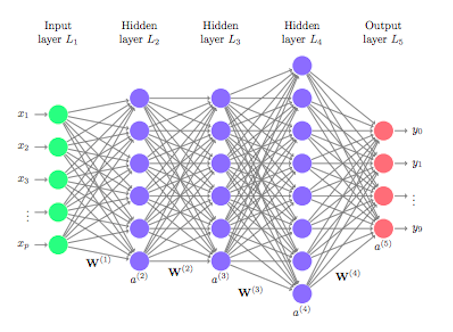
\includegraphics[width=12cm]{figs/deep_learning}
  \end{center}
  \caption{Simple ejemplo de una red neuronal en el algoritmo de Deep Learning.}
  \label{fig:red}
\end{figure}

Existen multitud de estudios sobre el Deep Learning. Uno de ellos ha sido la restauración de textos antiguos con el uso de una red neuronal profunda llamada Ithaca \cite{assael22} (Figura \ref{fig:textos}). Con ella se ha conseguido reparar textos dañados con una precisión del 62\% por sí sola. Está pensada para utilizarla con los historiadores, que han mejorado su precisión del 25\% al 72\% con esta nueva herramienta.\\
\begin{figure} [h!]
  \begin{center}
    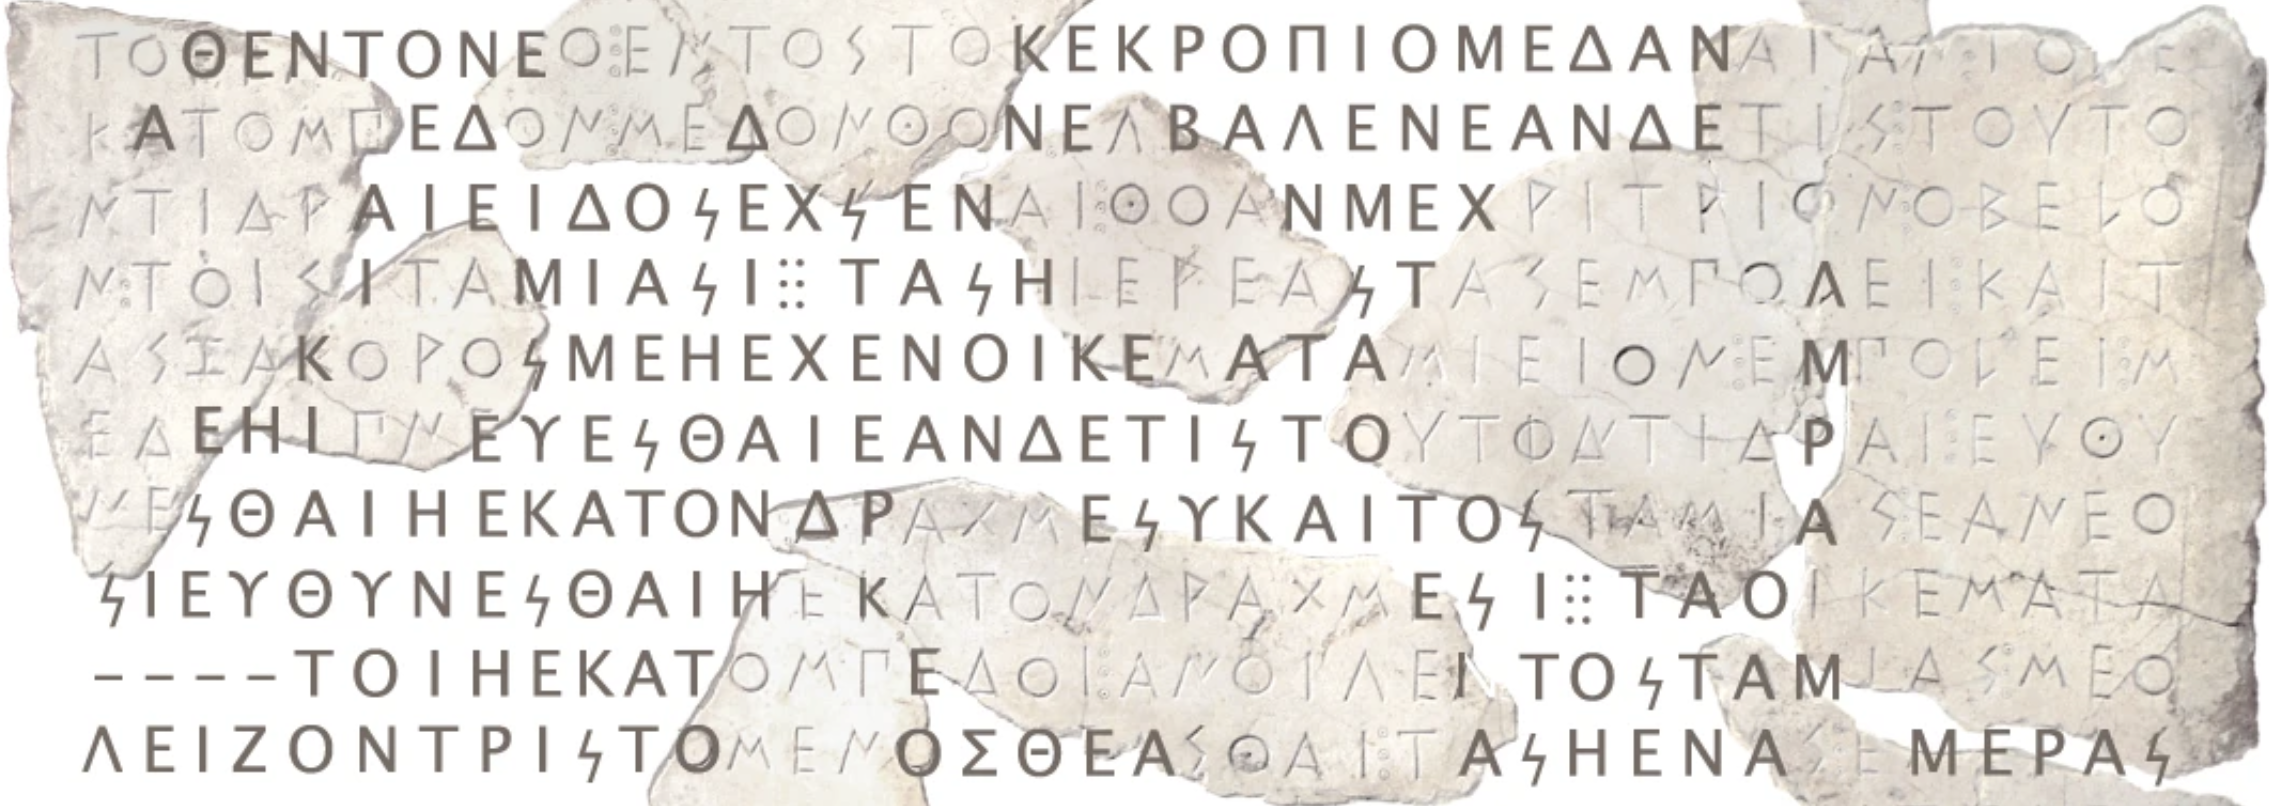
\includegraphics[width=11cm]{figs/textos}
  \end{center}
  \caption{Decreto sobre la Acrópolis de Atenas reconstruido con Ithaca.}
  \label{fig:textos}
\end{figure}

También existen aplicaciones de Deep Learning que se utilizan en la vida cotidiana, como los asistentes virtuales.  Este es el caos de los dispositivos Siri o Alexa ---entre otros--- que, mediante algoritmos de Deep Learning, ayudan a los usuarios a realizar distintas tareas, aprendiendo continuamente de la información que reciben.\\

Otro ejemplo donde se emplean algoritmos de DL es el reconocimiento de imágenes. Aquí se pueden encontrar numerosas aplicaciones prácticas, como por ejemplo el enfoque automático en las caras al realizar fotos (Figura \ref{fig:caras}).\\
\begin{figure} [h!]
  \begin{center}
    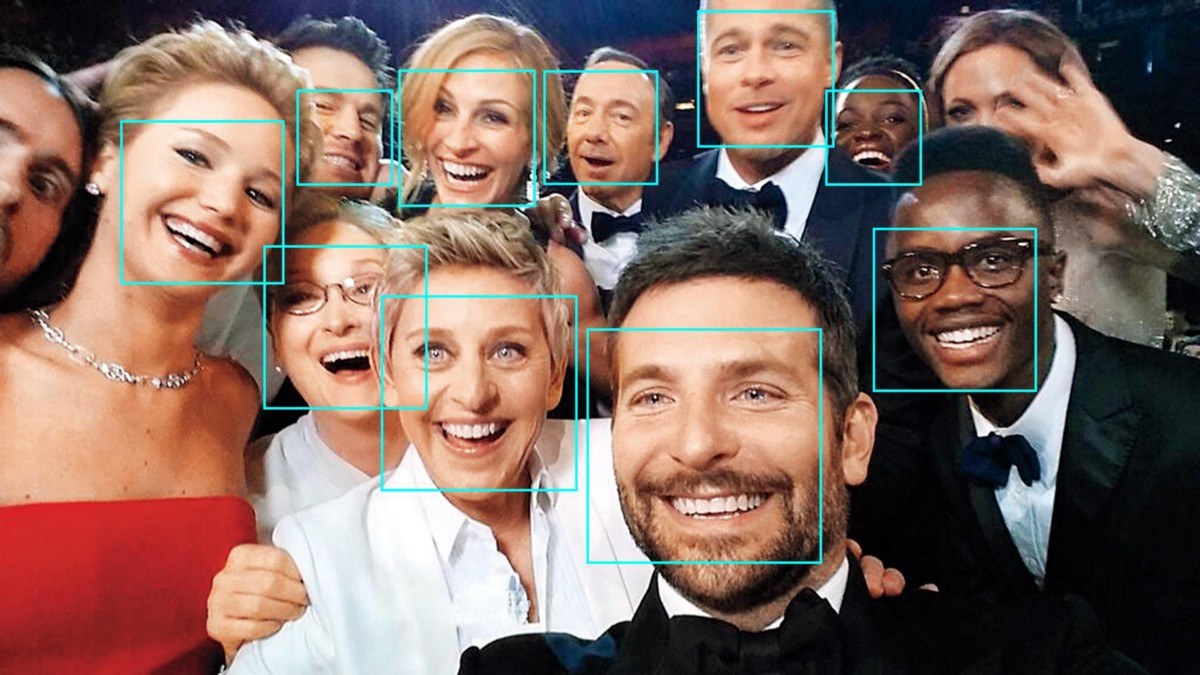
\includegraphics[width=8cm]{figs/caras}
  \end{center}
  \caption{Reconocimiento facial con técnica de Deep Learning.}
  \label{fig:caras}
\end{figure}

\section{Sistemas multisensoriales}
Como se ha explicado en las secciones anteriores, el desarrollo del Deep Learning es muy importante. Lo es especialmente en el campo de la visión artificial, pues permite crear aplicaciones sofisticadas que simulan la visión humana. Pero si además del sensor de visión se incorporan otros tipos de sensores a un robot, el resultado de la actuación de este mejora, ya que, además de percibir la imagen del entorno, está percibiendo más información que puede ser útil a la hora de tomar decisiones. Retomando la analogía con el ser humano, si este, además de ver, es capaz de sentir, oler o tocar, recibe más información de su entorno, por lo que puede conocer mejor la situación en la que se encuentra y, con ello, actuar más inteligentemente.\\

Numerosas son las aplicaciones de un sistema multisensorial, por ejemplo para los sistemas propioceptivos. Estos sistemas necesitan conocer con exactitud las variables del entorno. Otra aplicación se encuentra en los robots móviles. Al disponer de múltiples sensores, estos robots reducen el error en sus movimientos. Otro ejemplo del uso de sistemas multisensoriales es el seguimiento continuado de animales. Algunos ejemplos de estos sistemas se describen a continuación.\\

En \cite{ucm}, de la Universidad Complutense de Madrid se describe un sistema para detectar de forma temprana las enfermedades o infecciones en animales de granja, más concretamente en cerdos. Este sistema parte de la instalación de microchips y otro tipo de sensores en los animales para poder controlar las condiciones, como su temperatura o el consumo de agua de los bebederos, de forma que un ordenador muestra esta información de manera gráfica. También se incluye una monitorización grupal mediante grabaciones diarias para que el sistema detecte cualquier tipo de actividad no común (Figura \ref{fig:ucm}).\\
\begin{figure} [h!]
  \begin{center}
    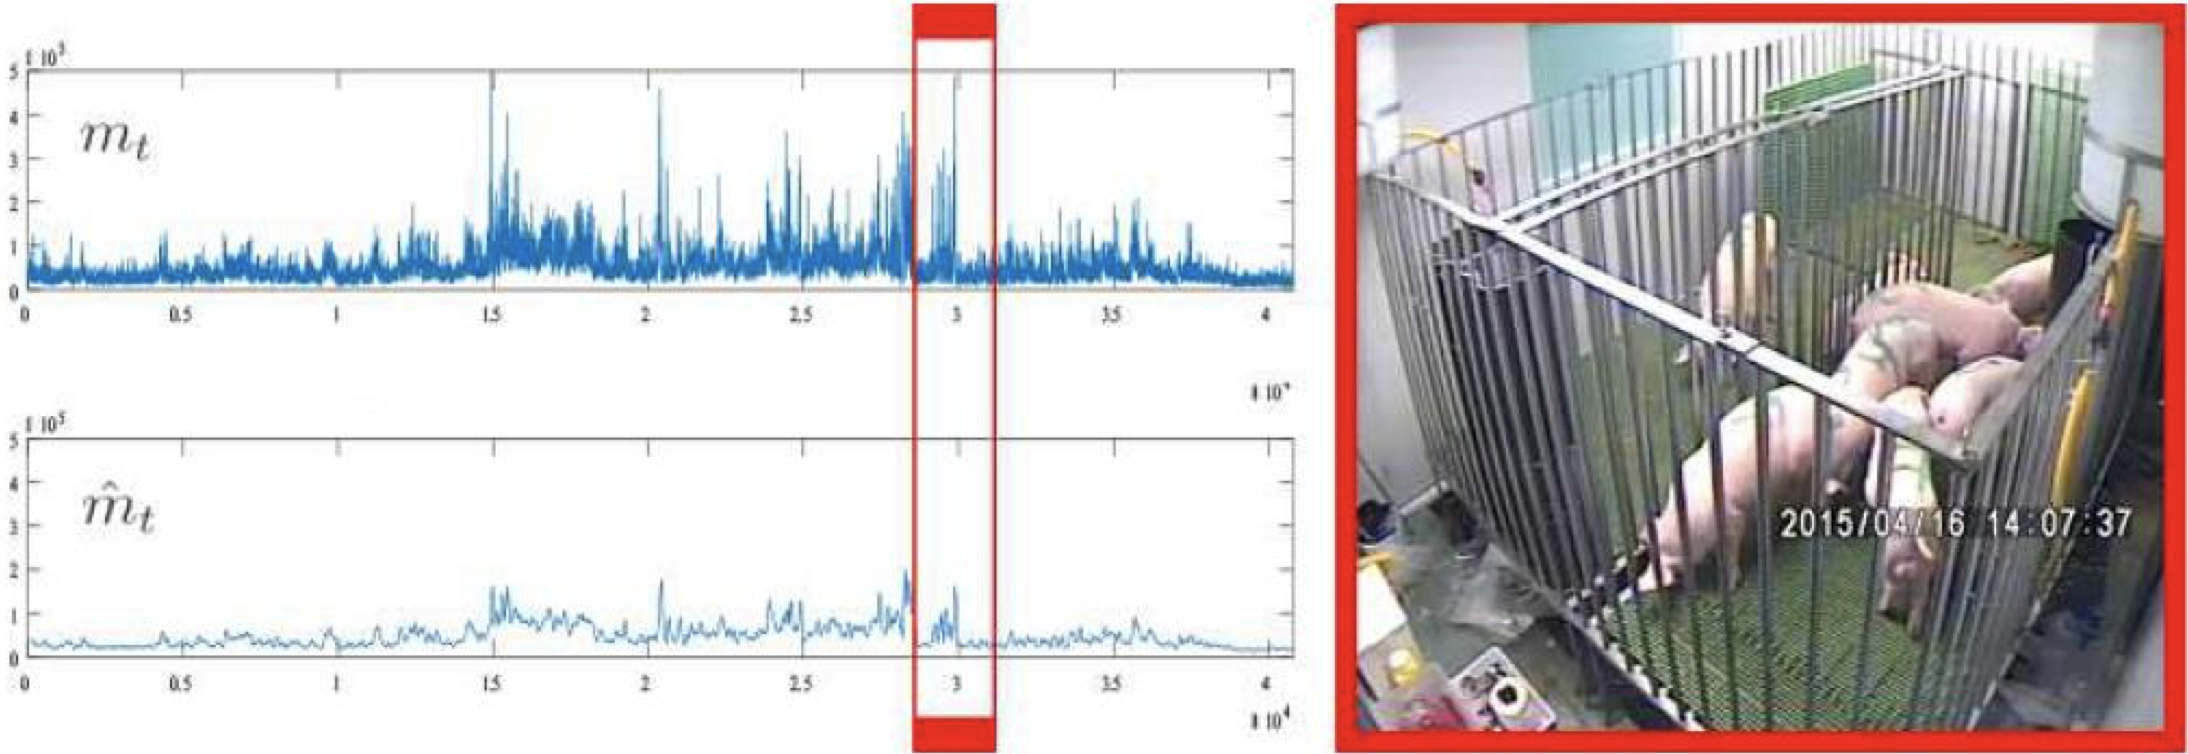
\includegraphics[width=14cm]{figs/ucm}
  \end{center}
  \caption{Patrón de movimientos e imagen grabada del grupo de cerdos.}
  \label{fig:ucm}
\end{figure}

En \cite{arce09}, la Facultad de Zootecnia e Ingeniería de la Universidad de São Paulo presenta un sistema de sensores con el fin de obtener datos fisiológicos de los animales (en este caso vacas) y obtener las condiciones en las que estos tienen menos perturbaciones en su comportamiento natural, pues las condiciones climatológicas en cada región pueden afectar de diferentes maneras: estrés, pérdidas productivas o incluso la muerte. Este sistema se creó con la instalación de sensores en cada una de las vacas creando una red de sensores (Figura \ref{fig:saopaulo}) que se comunican con una estación para obtener todos los datos del conjunto de animales.\\
\begin{figure} [h!]
  \begin{center}
    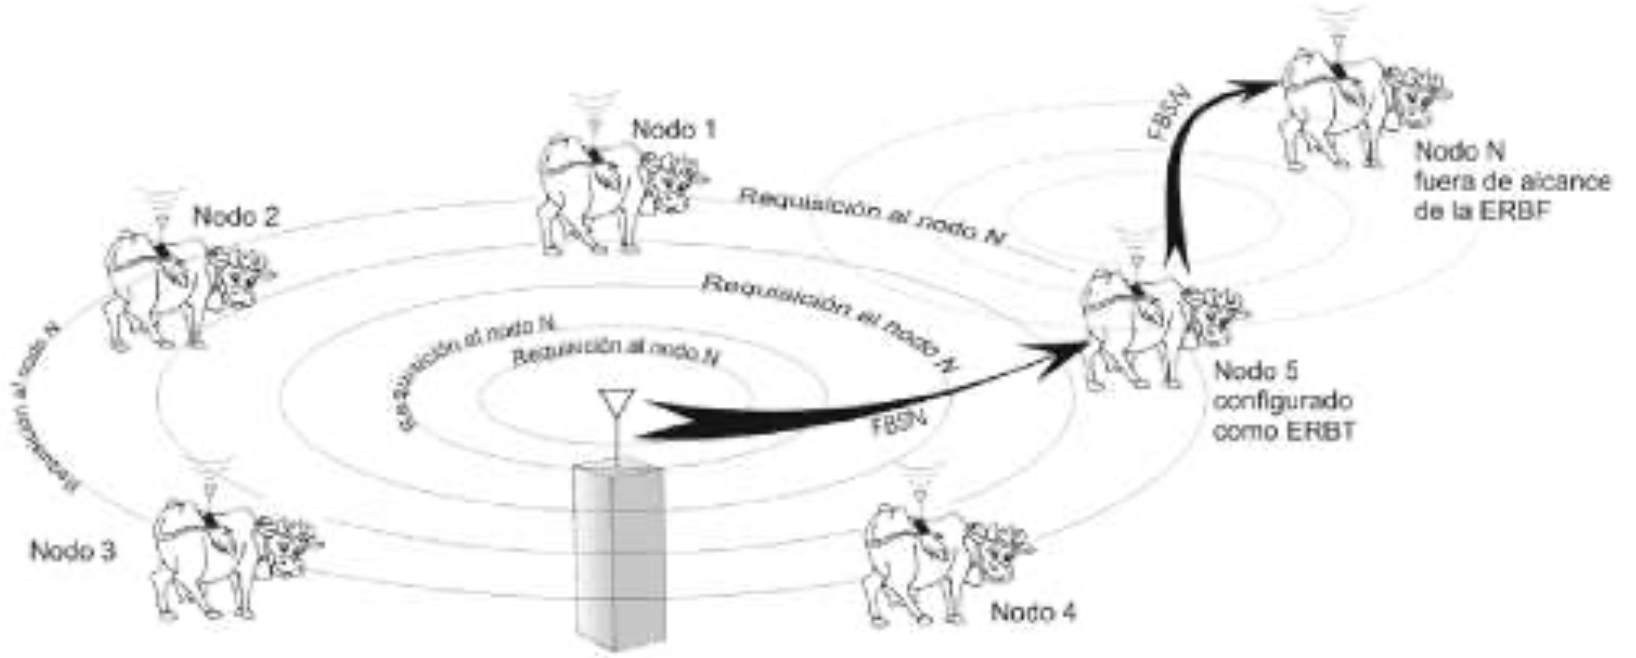
\includegraphics[width=14cm]{figs/saopaulo}
  \end{center}
  \caption{Esquema del desarrollo del sistema mediante sensores.}
  \label{fig:saopaulo}
\end{figure}

El comportamiento que tienen los animales puede ofrecer mucha información acerca de su salud si se mantiene una observación constante, pero también tienen una gran importancia las condiciones del entorno en la que se encuentran, ya que pueden ser decisivas para detectar el motivo de su comportamiento. Por ello, es importante tener un seguimiento constante y automatizado de estas características, permitiendo al humano encargarse únicamente de controlar los datos que el sistema registra.\\
\

\

\

\

\

\
El presente trabajo se enmarca en el contexto de los sistemas multisensoriales, concretamente en los sistemas multisensoriales destinados al bienestar animal y al análisis de comportamiento, en el cual juega un papel fundamental las técnicas de DL.\\

En los próximos capítulos se describe el sistema desarrollado. En el Capítulo 2 se comentan los objetivos, requisitos y metodología del trabajo. En el Capítulo 3 se explican las plataformas de desarrollo que se han utilizado para desarrollar el trabajo. En el Capítulo 4 se describe el proceso exhaustivo que ha llevado el trabajo y finalmente, en el Capítulo 5 se escriben las conclusiones.

\chapter{Objetivos}
\label{cap:capitulo2}

%\begin{flushright}
%\begin{minipage}[]{10cm}
%\emph{Quizás algún fragmento de libro inspirador...}\\
%\end{minipage}\\

%Autor, \textit{Título}\\
%\end{flushright}

\vspace{1cm}

En el capítulo anterior se ha dado el contexto del trabajo, mientras en este se presenta el plan de trabajo, definiendo los objetivos tanto generales como específicos que se han marcado para desarrollarlo y los requisitos que debe respetar el proyecto. Posteriormente se explica la metodología utilizada para cumplir con los objetivos.\\

\section{Descripción del problema}
\label{sec:descripcion}

El objetivo general de este proyecto es crear un sistema accesible económicamente para cualquier usuario que a través del uso de diferentes sensores sea capaz de medir las condiciones del entorno en la que se encuentran los animales en un laboratorio --- en concreto, ratones--- y mostrarlo en una interfaz gráfica en tiempo real que sea fácilmente manejable por cualquier usuario. Asimismo, que el sistema también sea capaz de controlar el tiempo en el que los animales pasan haciendo las diferentes tareas.\\
Actualmente el control de estas características es mediante un humano, no estando automatizado por ningún sistema. Es por ello que el objetivo de este trabajo tiene una necesidad real de la que actualmente carece el laboratorio.\\
Para cumplir este objetivo general, es necesario marcar una serie de objetivos específicos para el correcto desarrollo del trabajo:
\begin{itemize}
 \item Recoger la lectura de los sensores en un mismo fichero. Cada sensor necesita las librerías pertinentes para obtener una lectura correcta, por lo que se creará una clase por sensor de manera que sea más fácil unificar todas estas lecturas. Se utilizará la librería \textit{Thread} que permitirá ejecutar concurrentemente la lectura de todos los sensores con el uso de la función \verb|threads.append(Thread(target=funcion))|.
 \item Crear un servidor web para los dos sensores que recogen imágenes. Para la cámara térmica, la única función del servidor será mostrar la imagen que graba la cámara. Sin embargo, para la cámara normal, además de mostrar las imágenes, deberá incorporar un botón que permita iniciar y parar la grabación cuando el usuario quiera, guardando el vídeo automáticamente en el sistema. Además, la visualización desde el servidor aportará la hora y la fecha. Para llevar esto a cabo se utilizará la librería OpenCV. Con el uso de las funciones \verb|cv2.rectangle()| y \verb|cv2.putText()| se creará un rectángulo y se añadirá el texto deseado respectivamente.\\
 Estos servidores de flask estarán protegidos por un factor de doble autenticación para aportar seguridad.
 \item Detectar los diferentes ratones mediante un algoritmo de reconocimiento de objetos a través de TensorFlowLite para poder determinar el tiempo que pasan los animales haciendo las diferentes actividades.
\end{itemize}
\section{Requisitos}
\label{sec:requisitos}
El trabajo cumplirá la siguiente serie de requisitos:
\begin{itemize}
 \item El sistema sobre el que se realizará el trabajo será la Raspberry Pi 4B, haciendo de este un sistema económico. 
 \item El lenguaje de programación será Python, debido a la familiaridad del autor con él además de la amplia variedad de librerías ---útiles para este trabajo--- que permite usar.
 \item La interfaz de usuario será creada con Node-Red, y deberá ser fácil e intuitiva.
\end{itemize}
\section{Metodología}
\label{sec:metodologia}
Para la satisfacción de los objetivos y el cumplimiento de los requisitos mencionados anteriormente, se han usado diferentes herramientas para el correcto control y desarrollo del proyecto.\\

Para el seguimiento del trabajo se han llevado a cabo reuniones semanales con el tutor del trabajo en la plataforma Microsoft Teams\footnote{\url{https://www.microsoft.com/es-ar/microsoft-teams/log-in}}, donde se compartían los problemas surgidos durante la semana junto a posibles soluciones que evaluar, además del control y evaluación de los objetivos marcados la semana anterior. También se establecían los nuevos objetivos para la próxima semana. Asimismo, se ha utilizado el correo electrónico para problemas que surgían a lo largo de la semana.\\
Paralelamente se ha contactado con los investigadores del laboratorio de la Universidad de Alcalá de Henares \footnote{\url{https://www.uah.es/es/}}tanto por videoconferencia como por correo electrónico para conocer la situación y la prioridad de los problemas que les gustaría solucionar.\\

La evolución de todo el trabajo se ha registrado en GitHub\footnote{\url{https://github.com/jmvega/tfg-icebollada}} donde se ha ido escribiendo el progreso que se ha llevado para realizar el trabajo, junto a los problemas que han ido surgiendo acompañados de imágenes o vídeos, así como las soluciones que han servido para solventarlos. También se han aportado fotos y vídeos mostrando el funcionamiento de las distintas partes del sistema, así como el funcionamiento entero de este.

%\section{Plan de trabajo}
%\label{sec:plantrabajo}


\chapter{Plataforma de desarrollo}
\label{cap:capitulo3}

%\begin{flushright}
%\begin{minipage}[]{10cm}
%\emph{Quizás algún fragmento de libro inspirador...}\\
%\end{minipage}\\

%Autor, \textit{Título}\\
%\end{flushright}

\vspace{1cm}

En este capítulo se definen tanto la infraestructura utilizada como los métodos, tanto a nivel software como hardware, que se han utilizado para desarrollar este trabajo.\\

\section{Plataforma hardware}
\label{sec:hw}
Para satisfacer el objetivo de crear un sistema multisensorial con las características definidas en el capítulo anterior y que además sea \textit{low-cost}, la infraestructura hardware en este trabajo se ha centrado en sistemas embebidos empotrados existentes en el mercado. Dos de los sistemas más importantes son Raspberry (Figura \ref{fig:placas}-a) y Arduino (Figura \ref{fig:placas}-b). La decisión de trabajar con Raspberry en lugar de Arduino ha estado motivada por diferentes cuestiones.\\

Ambas placas disponen de pines GPIO ---del inglés General Purpose Input/Output--- o Entrada/Salida de Propósito General. Estos pines permiten la conexión de sensores o actuadores por medio de diferentes tipos de pines, que se pueden ver representados con distintos colores en la Figura \ref{fig:pinout}. Los tipos de pines que hay son los siguientes:
\begin{itemize}
\item 3.3V pin: Alimentación de 3.3V en los pines 1 y 17.
\item 5V pin: Alimentación de 5V en los pines 2 y 4.
\item Conexión a tierra: Utilizados para cerrar los circuitos eléctricos, para evitar quemar los componentes usados, en los pines 6, 9, 14, 20, 25, 30, 34 y 39.
\item Modulación del pulso (PCM): Convierten la señal digital a una señal analógica. Son los pines 12, 32, 33 y 35.
\item Conexión Circuito Integrado Interno ---del inglés Inter-Integrated Circuit--- (I2C) en los pines 3 (SDA) y 5 (SCL) o 27 (SDA) y 28 (SCL).
\item Conexión SPI (Interfaz de Comunicación Serie). Se encuentra en los pines 19, 21, 23 y 24.
\item Conexión UART (Transmisor-Receptor Asíncrono Universal) en los pines 8 y 10.
\item El resto de pines son pines que permiten la conexión de entrada o salida con el elemento conectado.
\end{itemize}

\begin{figure} [h!]
  \begin{center}
    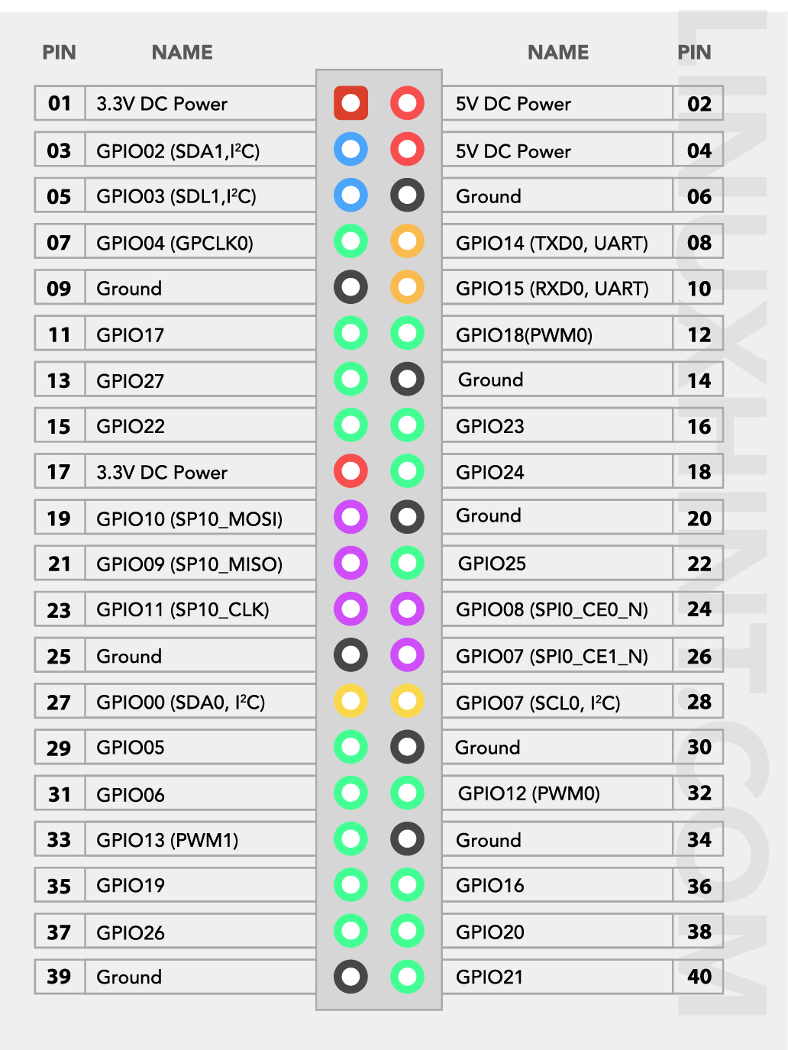
\includegraphics[width=10cm]{figs/pinout}
  \end{center}
  \caption{Tipos de pines GPIO en la Raspberry Pi 4.}
  \label{fig:pinout}
\end{figure}

A pesar de que ambas placas tienen pines GPIO, Arduino no permite la conexión de cámaras mientras que con Raspberry no solo se puede acoplar su cámara (PiCam) sino que permite conectar una webcam a través de uno de los puertos USB que tiene. Arduino es un microprocesador que cuenta con su IDE, mientras que Raspberry es un microordenador completo que cuenta con un completo sistema operativo Raspbian, basado en Debian. De esta forma, el usuario final puede visualizar los datos vertidos por el sistema con la conexión de la Raspberry a una pantalla a través de su puerto HDMI.\\
\begin{figure}[h!]
  \begin{center}
    \subfigure[Raspberry Pi]{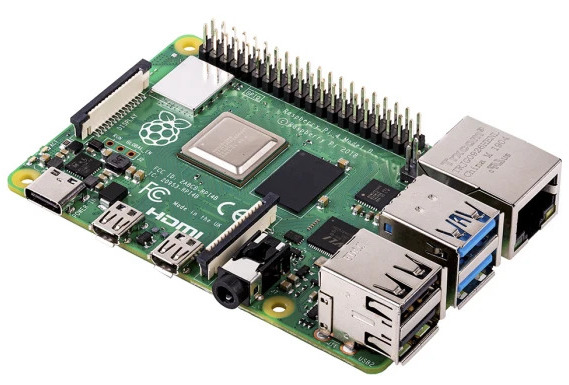
\includegraphics[width=75mm]{figs/raspberry_of}}\hspace{2mm}
    \subfigure[Arduino]{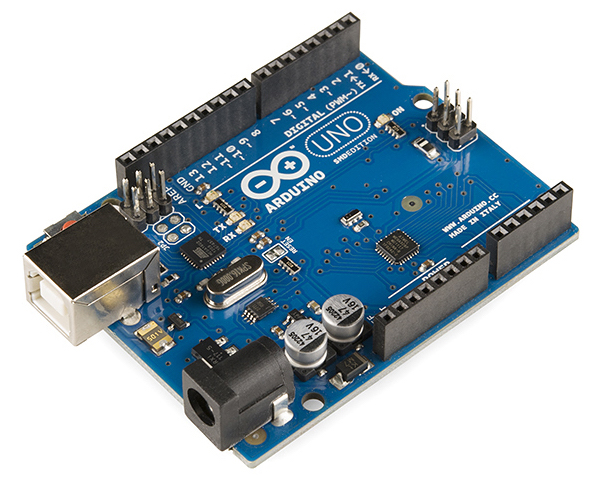
\includegraphics[width=70mm]{figs/arduino_of}}
  \end{center}
\caption{Sistemas empotrados.} \label{fig:placas}
\end{figure}

A la placa Raspberry se han conectado una serie de sensores para obtener distintos valores necesarios para la monitorización del sistema. Para la obtención de la temperatura se han utilizado el sensor BME680 (Figura \ref{fig:bme_of}) y el sensor DS18B20 (Figura \ref{fig:ds_of}). Este segundo sensor es resistente al agua, por lo que permite recoger la temperatura en superficies húmedas o mojadas. El rango en el que trabaja el BME680 así como su resolución se encuentra en el Cuadro \ref{cuadro:bme_tabla} extraído de la ficha de datos del sensor. Las características del DS18B20 se encuentran en el Cuadro \ref{cuadro:ds_tabla}.\\
\begin{figure} [h!]
  \begin{center}
    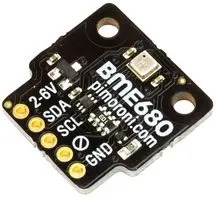
\includegraphics[width=6cm]{figs/bme_of}
  \end{center}
  \caption{Sensor BME680.}
  \label{fig:bme_of}
\end{figure}

\begin{figure} [h!]
  \begin{center}
    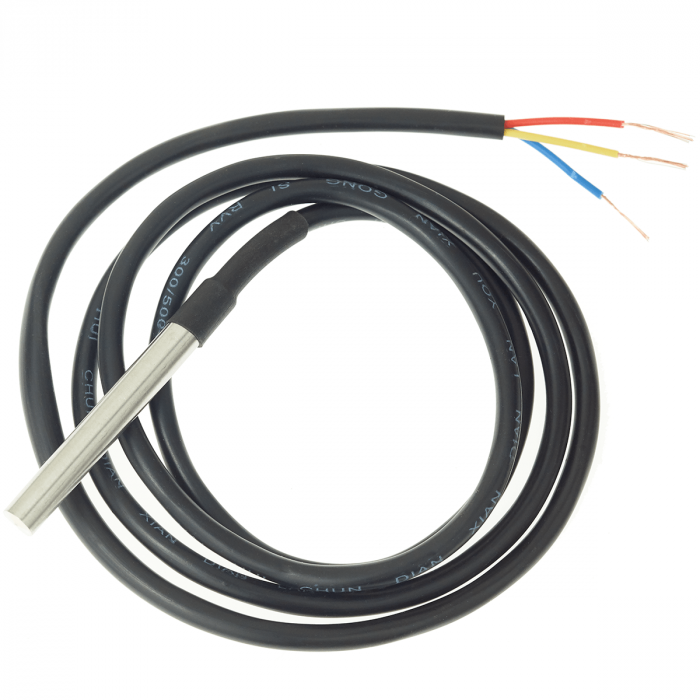
\includegraphics[width=6cm]{figs/ds_of}
  \end{center}
  \caption{Sensor DS18B20.}
  \label{fig:ds_of}
\end{figure}

\begin{table}[H]
\begin{center}
\begin{tabular}{|c|c|c|c|c|}
\hline
\textbf{Parámetros} & \textbf{Min}  & \textbf{Tipo}  & \textbf{Max}  & \textbf{Unidad}\\
\hline
Rango de temperatura de funcionamiento & -40 &  & 80 & ºC \\
Resolución de salida temperatura &  & 0.01 &  &ºC \\
Rango de presión de funcionamiento & 300 &  & 1100 & hPa \\
Resolución de salida presión &  & 0.18 &  &hPa \\
Rango de humedad de funcionamiento & 0 &  & 100 & \% r.H. \\
Resolución de salida humedad &  & 0.005 &  &\% r.H.  \\
\hline
\end{tabular}
\caption{Cuadro de características del sensor BME680.}
\label{cuadro:bme_tabla}
\end{center}
\end{table}

\begin{table}[H]
\begin{center}
\begin{tabular}{|c|c|c|c|}
\hline
\textbf{Parámetros} & \textbf{Min} & \textbf{Max}  & \textbf{Unidad}\\
\hline
Rango de temperatura de funcionamiento  & -55 & 125 & ºC \\
\hline
\end{tabular}
\caption{Cuadro de características del sensor DS18B20.}
\label{cuadro:ds_tabla}
\end{center}
\end{table}

Para la lectura de la humedad, la presión y la calidad del aire se ha utilizado el sensor BME680 (Figura \ref{fig:bme_of}), pues es capaz de medir más de un parámetro. La tabla de características se encuentra en el Cuadro \ref{cuadro:bme_tabla}.\\

Para el registro de imágenes térmicas, se han utilizado dos sensores. Uno de ellos es el sensor AMG8833 (Figura \ref{fig:termicos}-a) que ofrece una matriz de valores de temperatura. El segundo, es la cámara Seek Thermal (Figura \ref{fig:termicos}-b), que se ha conectado a la Raspberry a través de su puerto USB por medio de un adaptador.\\
\begin{figure}[h!]
  \begin{center}
    \subfigure[Sensor AMG8833.]{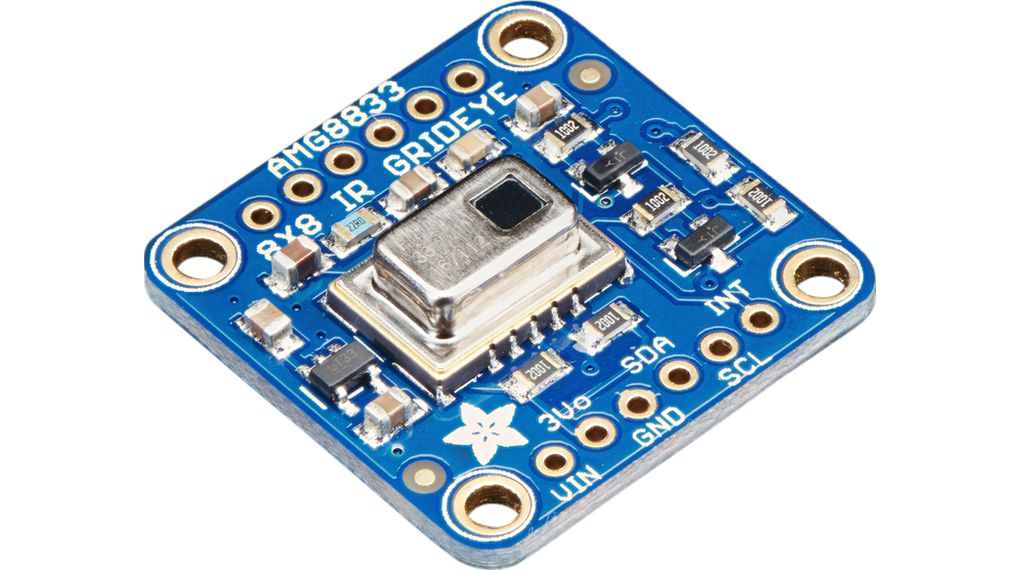
\includegraphics[width=7cm]{figs/amg_of}}\hspace{2mm}
    \subfigure[Cámara Seek Thermal]{
\includegraphics[width=6cm]{figs/seek_of}}
  \end{center}
\caption{Sensores térmicos utilizados en el trabajo.} \label{fig:termicos}
\end{figure}

Para el registro de imágenes se ha utilizado una de las cámaras de Raspberry, la Pi Camera (Figura \ref{fig:picam_of}). Ofrece una resolución de 8 megapíxeles, siendo una cámara de alta definición que ofrece poco ruido y alta sensibilidad.
\begin{figure} [h!]
  \begin{center}
    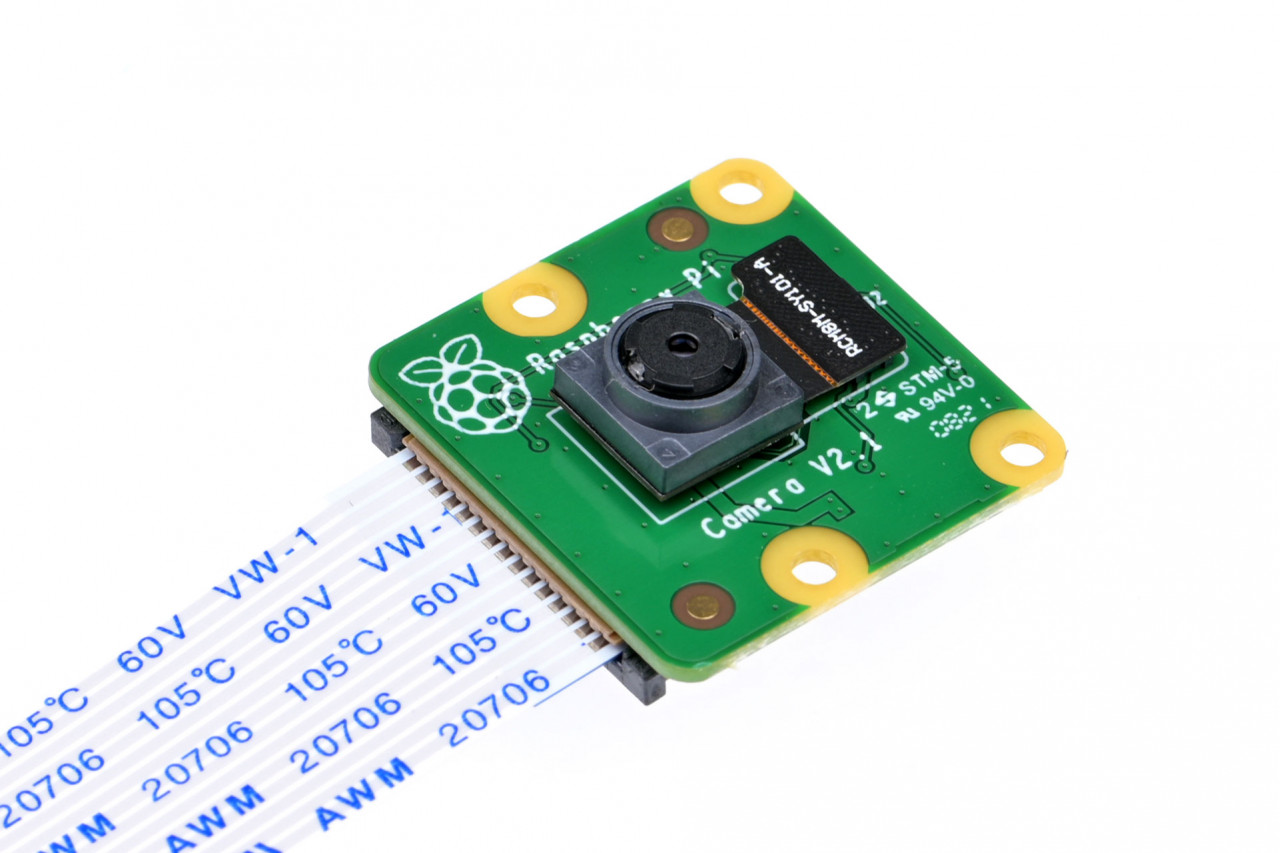
\includegraphics[width=6cm]{figs/picam_of}
  \end{center}
  \caption{Pi Camera.}
  \label{fig:picam_of}
\end{figure}

Otro sensor utilizado ha sido el sensor de nivel de agua (Figura \ref{fig:nivel_of}), que permite detectar la presencia de agua. También es posible obtener una idea de la cantidad de agua presente, aunque no de forma precisa.
\begin{figure} [h!]
  \begin{center}
    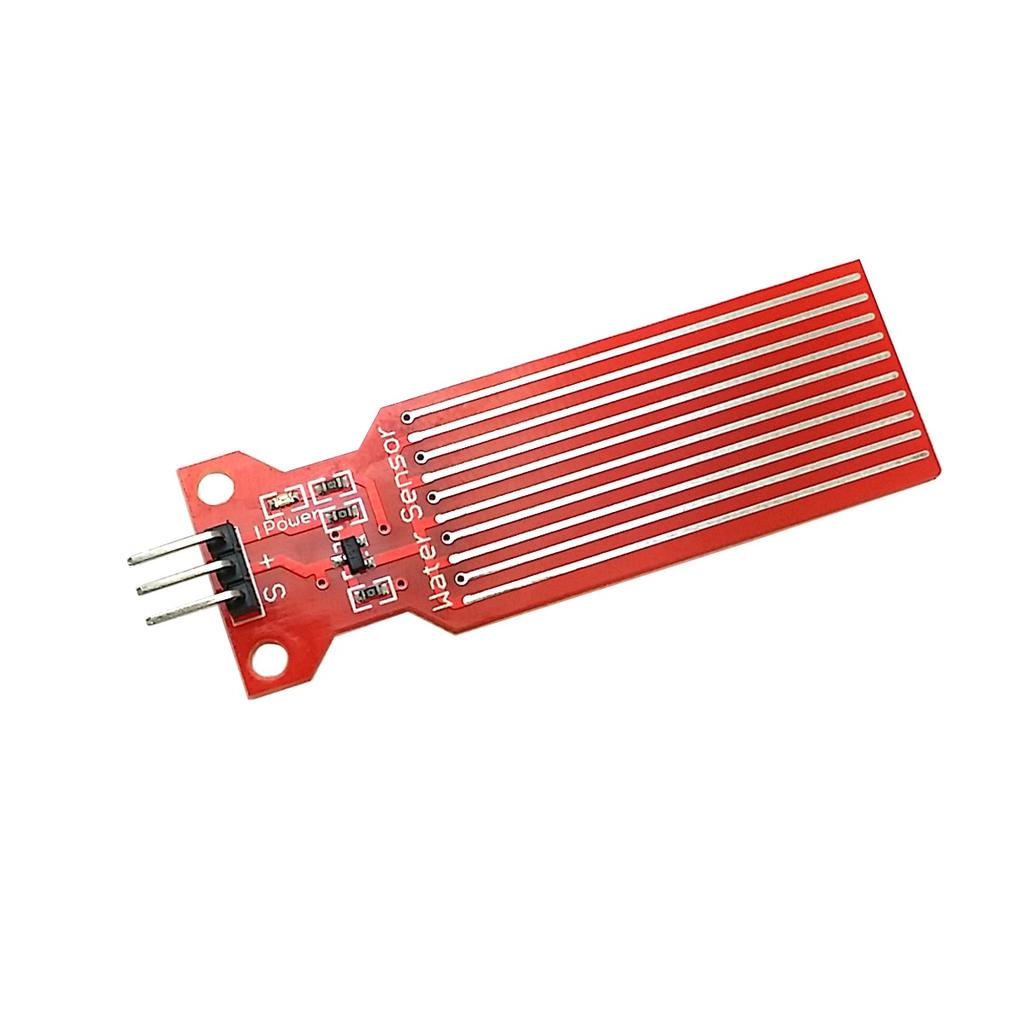
\includegraphics[width=6cm]{figs/nivel_of}
  \end{center}
  \caption{Sensor de nivel de agua.}
  \label{fig:nivel_of}
\end{figure}

El último sensor integrado en el trabajo ha sido el MQ-135 (Figura \ref{fig:mq_of}), que permite detectar la concentración de diferentes gases como el alcohol, benceno, humo, dióxido de carbono o amoníaco. En concreto, este sensor se ha utilizado para la detección de amoníaco.\\
\begin{figure} [h!]
  \begin{center}
    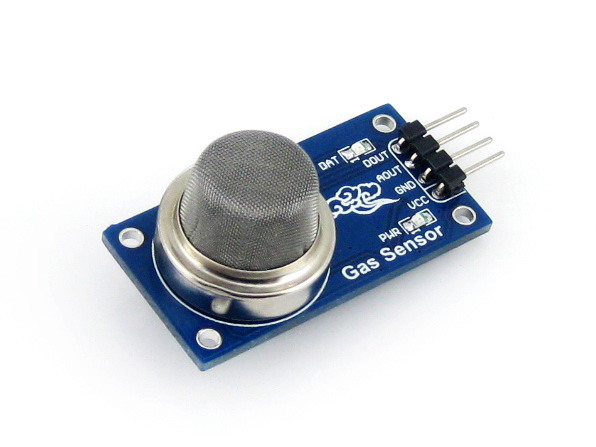
\includegraphics[width=6cm]{figs/mq_of}
  \end{center}
  \caption{Sensor MQ-135.}
  \label{fig:mq_of}
\end{figure}

Para conseguir el correcto funcionamiento de los sensores en la placa Raspberry, se ha utilizado la infraestructura software descrita a continuación.\\

\section{Infraestructura software}
Para dar soporte a la placa Raspberry se ha usado su sistema operativo oficial Raspberry Pi OS, también llamado Raspbian (Figura \ref{fig:raspbian}) bajo la versión de 64 bits. La elección de usar este Sistema Operativo (SO), entre otras, es que está optimizado para funcionar en procesadores ARM, que es el que tiene Raspberry, por lo que es el que mejor rendimiento ofrece para la placa. Además, Raspberry Pi OS está basado en Debian, por lo que tenemos todas las bondades de un sistema Linux.\\
\begin{figure} [h!]
  \begin{center}
    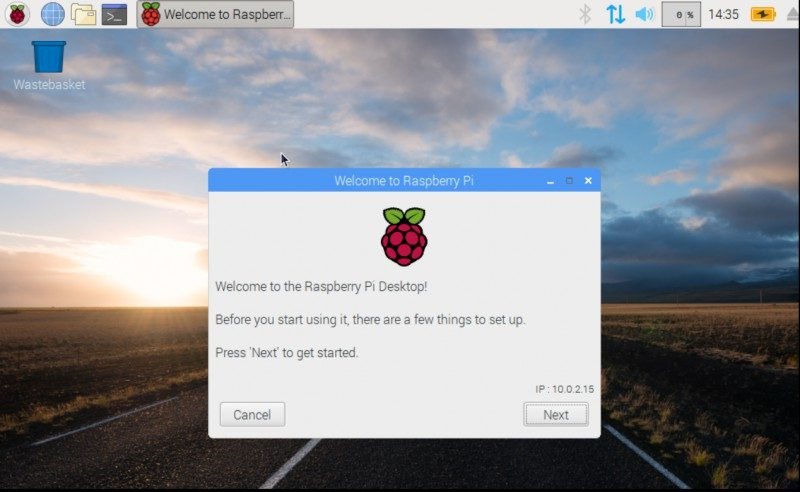
\includegraphics[width=14cm]{figs/raspbian}
  \end{center}
  \caption{Imagen de Raspberry Pi OS.}
  \label{fig:raspbian}
\end{figure}

A continuación se presentan las herramientas utilizadas para el desarrollo y funcionamiento del presente trabajo.

\subsection{Lenguaje Python}
\label{sec:python}
Python es un lenguaje de alto nivel de programación, interpretado y orientado a objetos, cuya filosofía hace hincapié en la legibilidad de su código y, por ello, su sintaxis es sencilla. Ofrece numerosos módulos y librerías para las distintas aplicaciones. Algunas de estas librerías son: YOLO para aplicaciones en ML (Código \ref{cod:modelo}), Pandas para análisis de datos, Flask para aplicaciones web o SQLAlchemy para comunicación entre bases de datos y programas. El uso de estos módulos y librerías facilita la reusabilidad de código y la programación modulada. No requiere del proceso de compilación, lo que lo convierte en un lenguaje muy rápido en el ciclo de edición, prueba y depuración.\\
\begin{code}[h]
\begin{lstlisting}[language=Python]
!python train.py --img 480 --batch 16 --epochs 100 --data /content/yolov5/data/custom.yaml --weights yolov5s.pt --cache
\end{lstlisting}
\caption[Código para el entrenamiento de un modelo de detección de ratones.]{Código para el entrenamiento de un modelo de detección de ratones.}
\label{cod:modelo}
\end{code}

Actualmente, es el lenguaje de programación más usado en el mundo, según la calificación de la empresa TIOBE\footnote{\url{https://www.tiobe.com/tiobe-index/}}, por lo que cuenta con una gran comunidad. Además, también es el más popular en el ámbito del Machine Learning. Algunas de las aplicaciones que usan Python son: Google, Netflix, Dropbox o Spotify.\\

La decisión de usar Python para el desarrollo de este TFG ha sido que es uno de los lenguajes de programación que mejor funciona y está soportado de forma nativa en el SO utilizado Raspbian, además de las numerosas librerías útiles para este proyecto adaptadas a Raspberry que Python posee.\\

En este trabajo, Python se utiliza para la lectura de los sensores de forma concurrente, para la creación de los dos servidores web que tiene tanto la PiCamera como la cámara térmica con Flask, y para el reconocimiento de lo ratones a través de la librería de YOLOv5.\\

\subsection{YOLOv5}
\label{sec:yolo}
YOLO ---siglas del acrónimo en inglés \textit{You Only Look Once}--- es un algoritmo de detección de objetos en tiempo real. Es un sistema de código abierto que hace uso de una red neuronal convolucional ---del inglés, Convolutional Neural Network (CNN)--- para la detección de objetos en imágenes o vídeos. En una explicación simplificada, esta red neuronal divide la imagen en MxM celdas de tamaño fijo. Cada celda debe predecir un solo objeto, mostrándolo posteriormente en la imagen a través de un cuadro delimitador o \textit{bounding box}, tal y como se puede ver en la Figura \ref{fig:regiones}.\\
\begin{figure} [h!]
  \begin{center}
    \includegraphics[width=15cm]{figs/regiones}
  \end{center}
  \caption{División en celdas y detección de objetos en una CNN.}
  \label{fig:regiones}
\end{figure}
Las red está formada por 24 capas convolucionales, que se encargan de extraer las características de la imagen, y 2 capas de conexión completa que predicen las coordenadas del objeto. Tiene 5 modelos diferentes que ofrecen diferentes características según el interés del uso. Se pueden ver las cualidades de cada modelo en la Figura \ref{fig:tablayolo}. \\
\begin{figure} [h!]
  \begin{center}
    \includegraphics[width=15cm]{figs/tablayolo}
  \end{center}
  \caption[]{Gráfica con las características de los distintos modelos de YOLOv5\footnotemark.} \label{fig:tablayolo}
\end{figure}\footnotetext{Imagen obtenida de \url{https://github.com/ultralytics/yolov5\#pretrained-checkpoints}.}

\subsection{OpenCV}
\label{sec:opencv}
OpenCV (Open Source Computer Vision Library) es una librería de software de visión computacional y machine learning de código abierto. Es ampliamente usada en todo el mundo debido al soporte multiplataforma que ofrece (Windows, Linux, MacOS y Android), además de ofrecer interfaz en diferentes lenguajes como Python, Java, C++ y MATLAB.\\

Compuesto por más de 2500 algoritmos, OpenCV está especializado en la visión computacional y en algoritmos de aprendizaje, permitiendo reconocer rostros, identificar o clasificar objetos, extraer modelos 3D, mejorar la calidad de las imágenes o detectar bordes (Figura \ref{fig:ej-opencv}), entre otros.\\

OpenCV se ha usado en este trabajo para manipular en tiempo real los vídeos grabados por las cámaras, permitiendo ---entre otras cosas--- integrar un \textit{timestamp} en estos. También ha permitido ofrecer la funcionalidad de guardar los vídeos cuando el usuario lo solicite a través del interfaz. Por último, y dada su fácil adaptación a otras aplicaciones, ha sido posible mostrar los vídeos de ambas cámaras (térmica y RGB) en el servidor web de Flask sin problema. Esta librería se detalla a continuación.\\
\begin{figure}[h!]
  \begin{center}
    \subfigure[Imagen original]{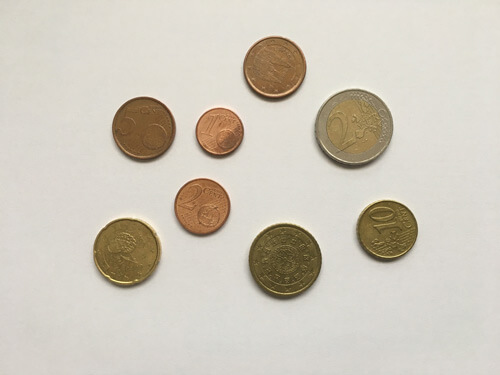
\includegraphics[width=45mm]{figs/monedas}}\hspace{9mm}
    \subfigure[Escala de grises]{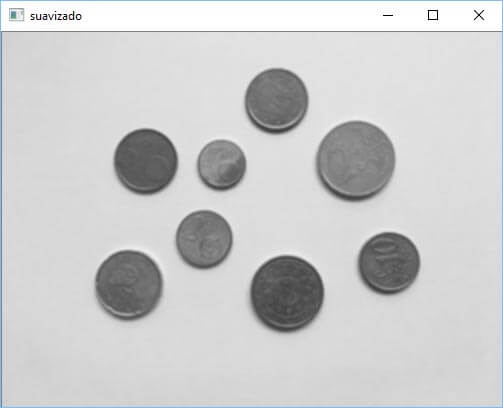
\includegraphics[width=45mm]{figs/suavizado}}\hspace{9mm}
    \subfigure[Detector de bordes]{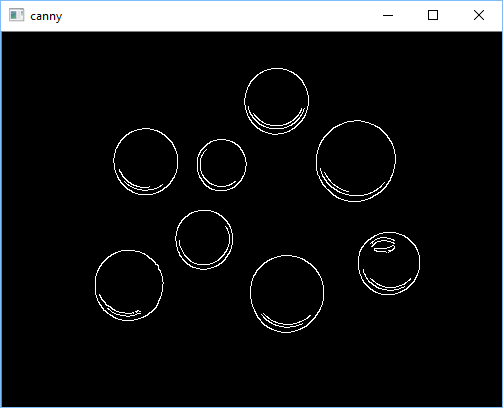
\includegraphics[width=45mm]{figs/detector-bordes}}\hspace{9mm}
    \subfigure[Contornos]{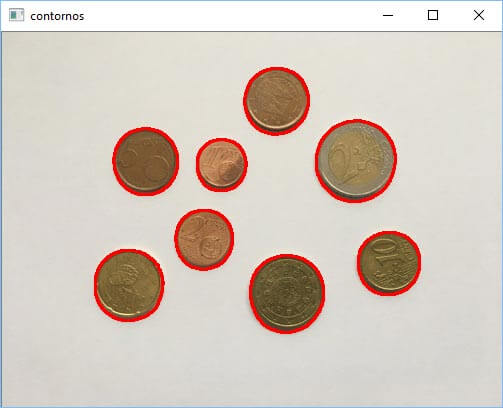
\includegraphics[width=45mm]{figs/contornos}}
  \end{center}
\caption{Ejemplo de detección de bordes con OpenCV.} \label{fig:ej-opencv}
\end{figure}

\section{Flask}
\label{sec:flask}
Flask es un marco de aplicación web minimalista ---en inglés, \textit{microframework}--- escrito en Python. Esto significa que ofrece al usuario herramientas y librerías para crear una aplicación web y, al ser minimalista, no requiere de otras dependencias para realizar las cosas básicas. Ofrece una serie de extensiones que permiten dotar de más características a la aplicación, como autenticación o manejo a través de comandos, entre otros.\\

Se compone de dos partes: las plantillas ---en inglés, \textit{templates}---, que están escritas en lenguaje HTML e indican la organización y diseño que tendrá cada página al ser visualizada, y el código en Python, que indica las rutas de cada página y las funciones de cada ruta. Este es el fichero que se ejecuta para crear el servidor.\\

En este proyecto se ha utilizado Flask para la creación de los dos servidores web de las cámaras. Se ha preferido Flask frente a Django, que es el más conocido para el uso con Python, debido a que el primero es más sencillo de utilizar y de aprender. Entre otras, este servidor permite realizar funciones como loguearse y registrase en él o acceder y controlar la visualización de las cámaras. En la Figura \ref{fig:flask-internet} se puede ver un ejemplo de un trabajo realizado con Flask.\\
\begin{figure} [h!]
  \begin{center}
    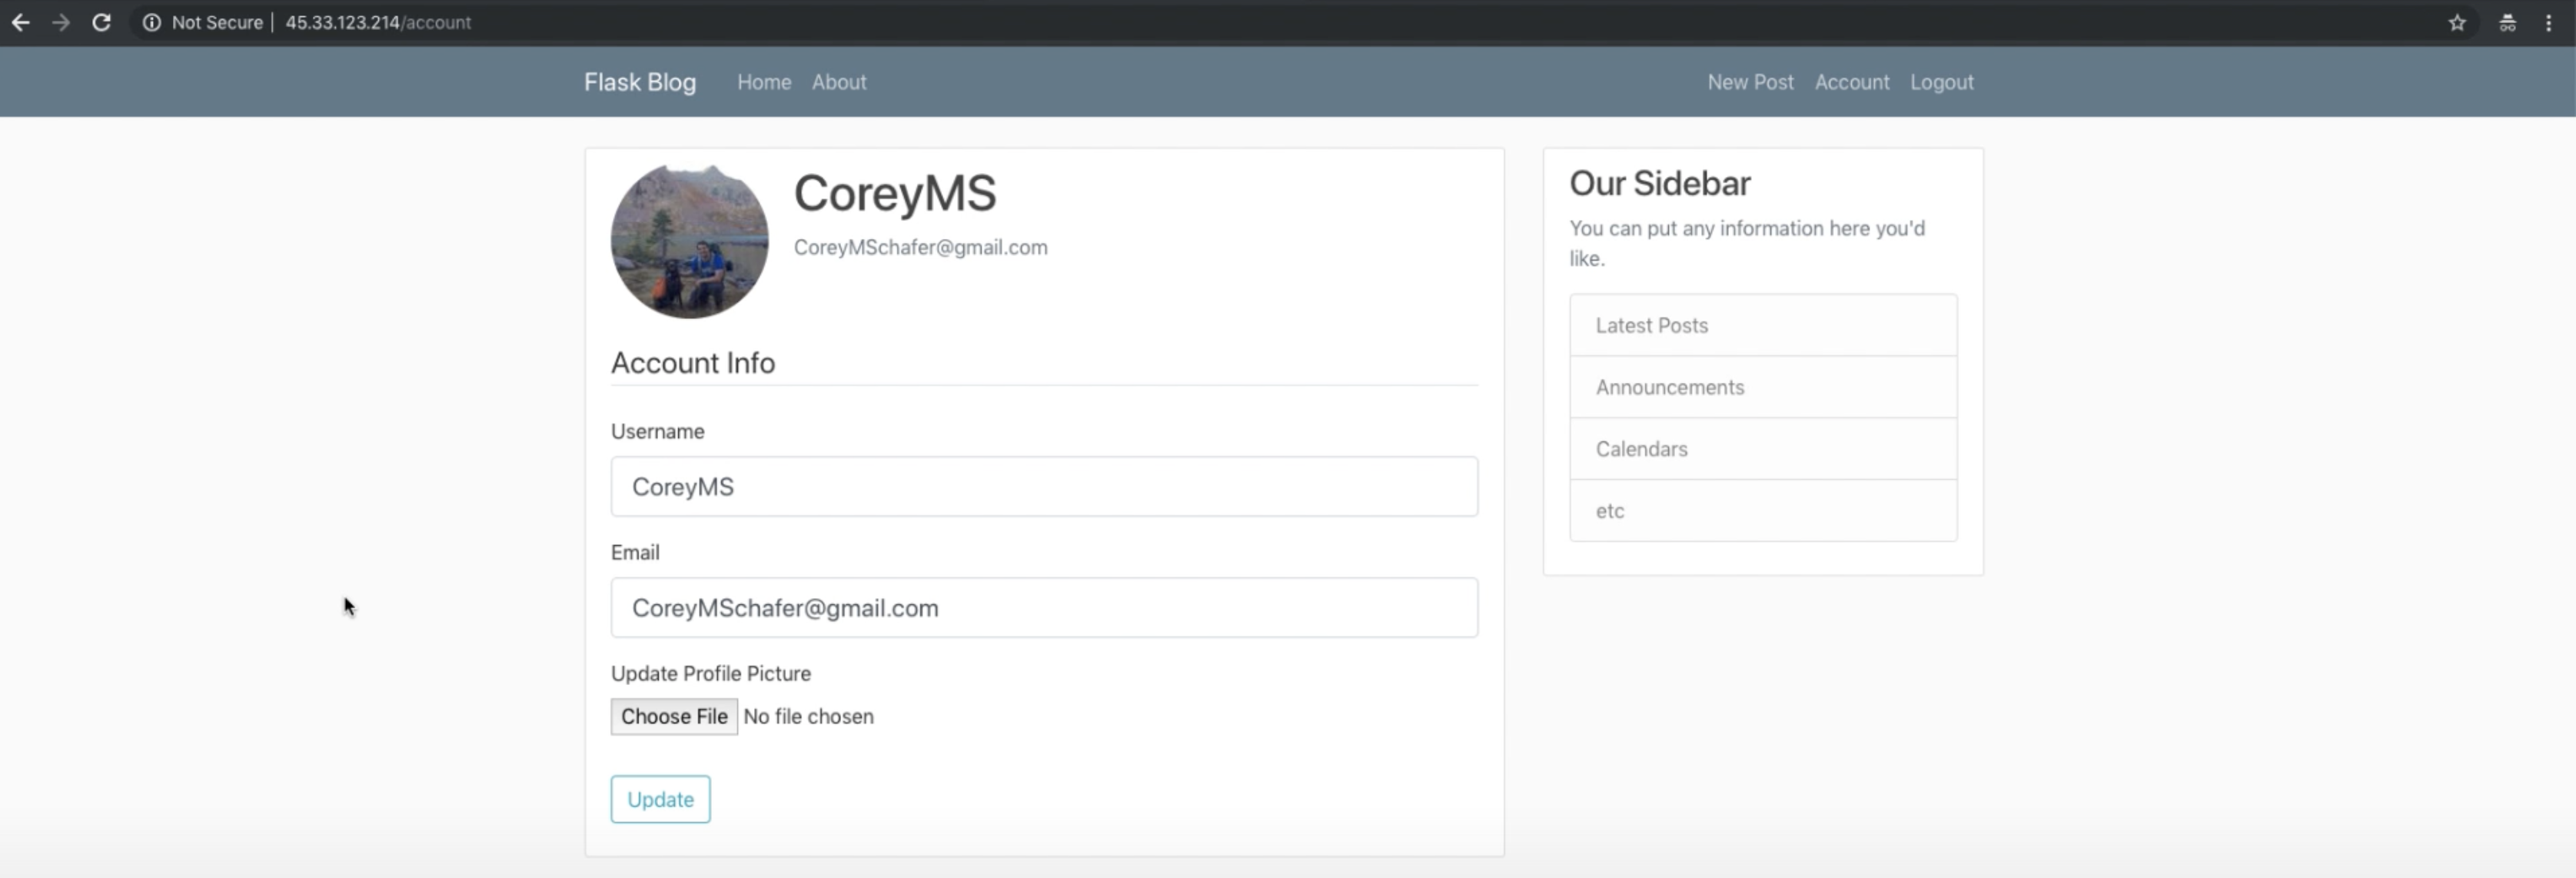
\includegraphics[width=15cm]{figs/flask-internet}
  \end{center}
  \caption{Blog creado con Flask.}
  \label{fig:flask-internet}
\end{figure}

\subsection{Node-Red}
\label{sec:nodered}
Node-Red es una herramienta de programación creada por IBM y escrita en lenguaje JavaScript que permite conectar dispositivos hardware y servicios en línea. Muestra de manera visual las conexiones de los nodos en un panel, mostrando gráficamente el flujo de la información. Además, es un entorno de ejecución ligero, lo que lo hace ideal para ejecutarse en hardware de bajo coste como la Raspberry.\\

Está compuesto por dos partes principales. Una de ellas es la edición de flujo desde navegador, donde muestra los nodos disponibles en el margen izquierdo así como la disposición y conexión del flujo creado por el usuario. La otra parte es el cuadro de mando, más comunmente \textit{dashboard}, que muestra la interfaz de usuario en base al flujo de los nodos de la parte previamente comentada.\\

Node-Red tiene una amplia variedad de nodos. Algunos de ellos permiten distintos tipos de conexiones, la interacción directa con los pines de Raspberry, la conexión con twitter o el correo electrónico. También permite la creación de ficheros de distintos tipos o la ejecución de ficheros ya existentes en la computadora.\\

Node-Red también permite el modo \textit{scripting}; esto es, la ejecución directa de código escrito en lenguaje JavaScript. Pueden crearse nuevos nodos para agregar nuevas capacidades gracias a los más de 225.000 módulos que hay en el repositorio de paquetes.\\

Los flujos de datos se pueden importar o exportar con ficheros en formato estándar JSON, permitiendo compartirlos con cualquier persona. La página de Node-Red tiene una librería de flujos que han creado otros usuarios, permitiendo el acceso a ellos para utilizarlos como base en otros proyectos (Figura \ref{fig:flujos}). En la Figura \ref{fig:ui-internet} se puede ver un ejemplo de un trabajo realizado en Node-Red.\\
\begin{figure}[h!]
  \begin{center}
    \subfigure[Flujo de Hola Mundo en Node-Red]{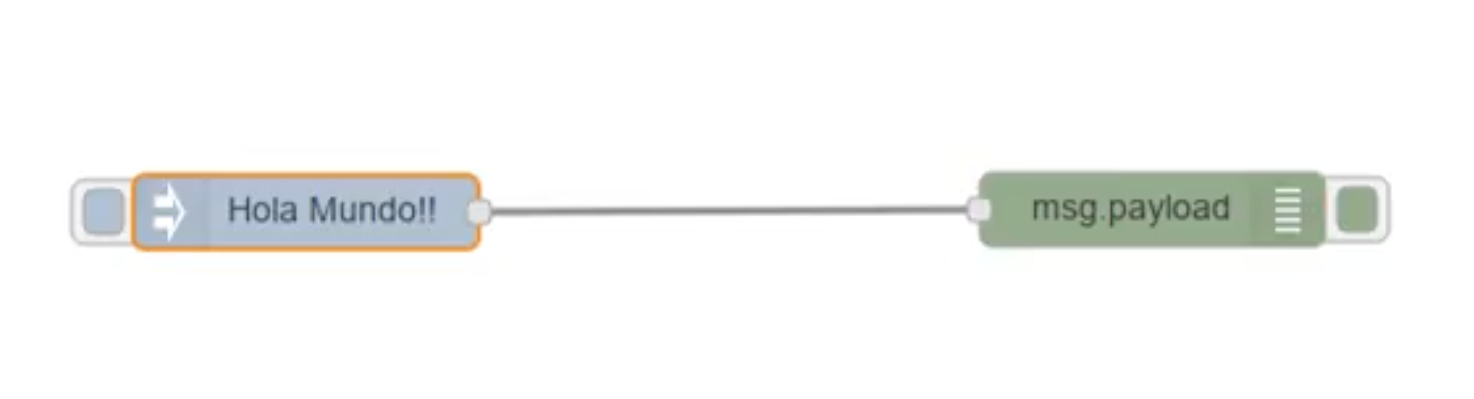
\includegraphics[width=14cm]{figs/holamundo-flujo}}\hspace{2mm}
    \subfigure[Flujo del proyecto de creación de un sistema de alarma]{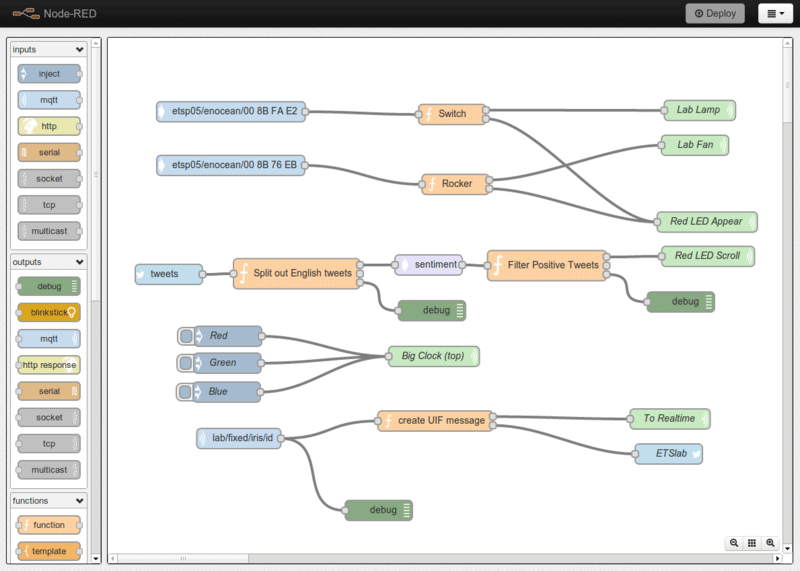
\includegraphics[width=14cm]{figs/alarma-flujo}}
  \end{center}
\caption{Distintos flujos hechos en Node-Red} \label{fig:flujos}
\end{figure}
\begin{figure} [h!]
  \begin{center}
    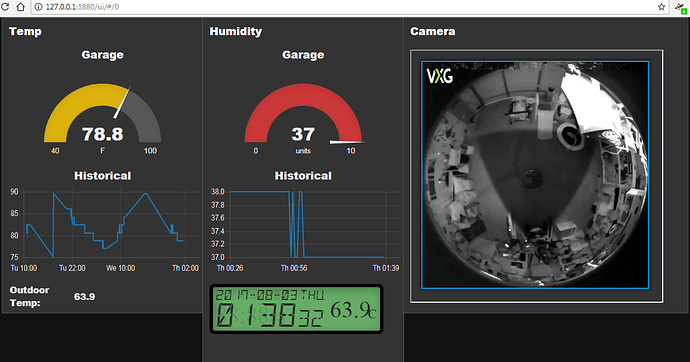
\includegraphics[width=15cm]{figs/ui-internet}
  \end{center}
  \caption{IU de un sistema de control de un garaje.}
  \label{fig:ui-internet}
\end{figure}

Para el desarrollo de este TFG, Node-Red ha tenido un papel muy importante. Además de tener una gran comunidad que permite la resolución de la mayoría de dudas, ha permitido la creación de la interfaz de usuario donde se muestran las mediciones de cada sensor, los dos servidores web de las cámaras y los botones e interruptores necesarios que permiten al usuario interactuar con la interfaz de una manera sencilla para obtener toda la información.\\

\chapter{Sistema multisensorial }
\label{cap:capitulo4}

%\begin{flushright}
%\begin{minipage}[]{10cm}
%\emph{Quizás algún fragmento de libro inspirador...}\\
%\end{minipage}\\

%Autor, \textit{Título}\\
%\end{flushright}

\vspace{1cm}
En este capítulo se describe detalladamente el proceso que se ha llevado a cabo para crear el sistema multisensorial para la monitorización de animales de laboratorio. Como se ha introducido previamente, la aplicación de este trabajo está enfocada a un laboratorio de investigación animal. Concretamente, se ha contactado con el Laboratorio del Bienestar e Investigación Animal de la Universidad de Alcalá de Henares\footnote{\url{https://www.uah.es/es/investigacion/unidades-de-investigacion/grupos-de-investigacion/Bienestar-en-Investigacion-Animal-Welfare-on-Animal-Research./}} para establecer los requisitos software del sistema. Así, el objetivo del trabajo se ha enfocado en la monitorización completa de los ratones del laboratorio, que requieren de una observación constante, así como del entorno en el que se encuentran, debido a que deben estar bajo unas condiciones determinadas.\\

Asimismo, para facilitar la comprensión de los datos por parte de los usuarios finales, se ofrece una interfaz gráfica donde los valores numéricos obtenidos por los sensores, así como cualquier interacción necesaria en la IU (Interfaz de Usuario) se traducen en \textit{widgets} ---pequeñas imágenes que proveen información visual--- comprensibles para cualquier usuario de una manera intuitiva y sencilla. El sistema creado se presenta en la Figura \ref{fig:misistema}.\\
\begin{figure} [h!]
  \begin{center}
    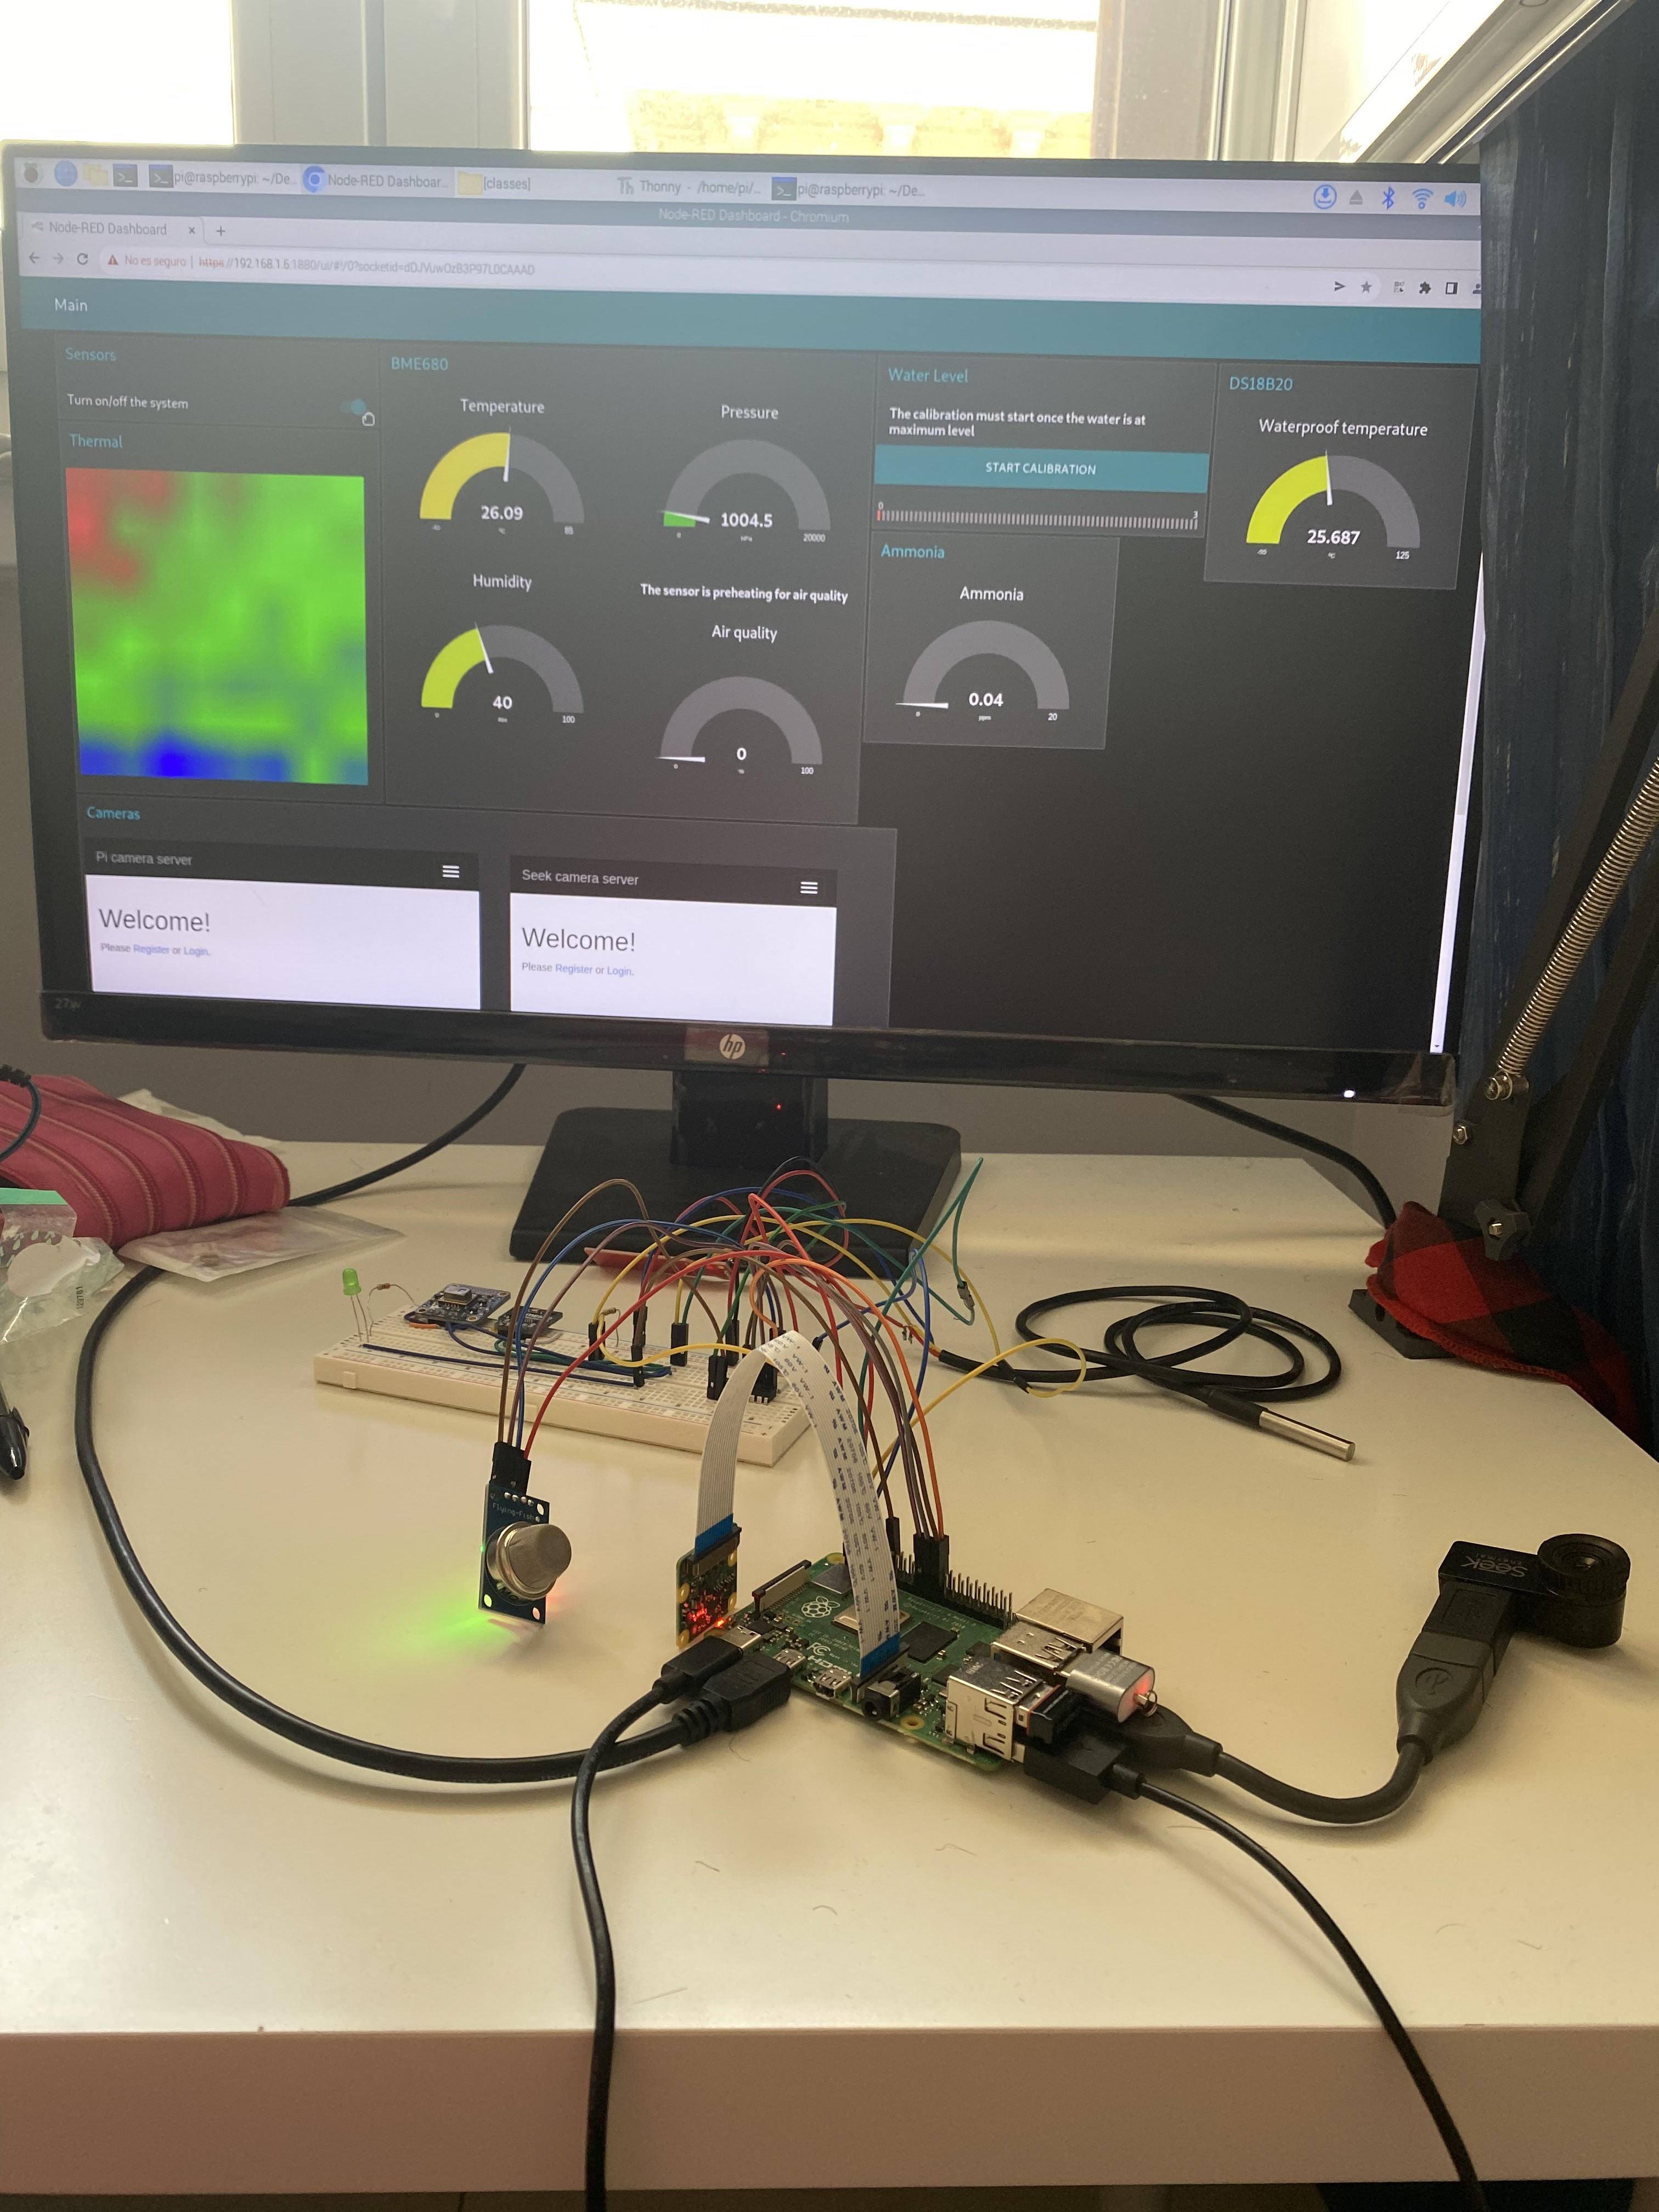
\includegraphics[width=10cm]{figs/misistema}
  \end{center}
  \caption{Sistema resultante.}
  \label{fig:misistema}
\end{figure}

Dos son las partes esenciales para el desarrollo del sistema: hardware y el software. En la Sección \ref{sec:deshw} se presenta el desarrollo hardware, y en la Sección \ref{sec:dessw} el desarrollo software que se ha realizado para tener un funcionamiento correcto del sistema.

\section{Desarrollo hardware}
\label{sec:deshw}
La placa que se ha utilizado para el proyecto es la Raspberry Pi 4B (Figura \ref{fig:rasp}-a), el último modelo de Raspberry y muy utilizada para el desarrollo de proyectos debido ---entre otras cosas--- a su bajo coste. Este modelo es el más rápido y potente, ofreciendo de dos a tres veces el rendimiento del procesador de su modelo predecesor, la Raspberry Pi 3b+. El sistema operativo utilizado para el desarrollo del proyecto ha sido Raspbian (Figura \ref{fig:rasp}-b).\\
\begin{figure}[h!]
  \begin{center}
    \subfigure[Raspberry Pi 4B utilizada para el desarrollo del presente TFG.]{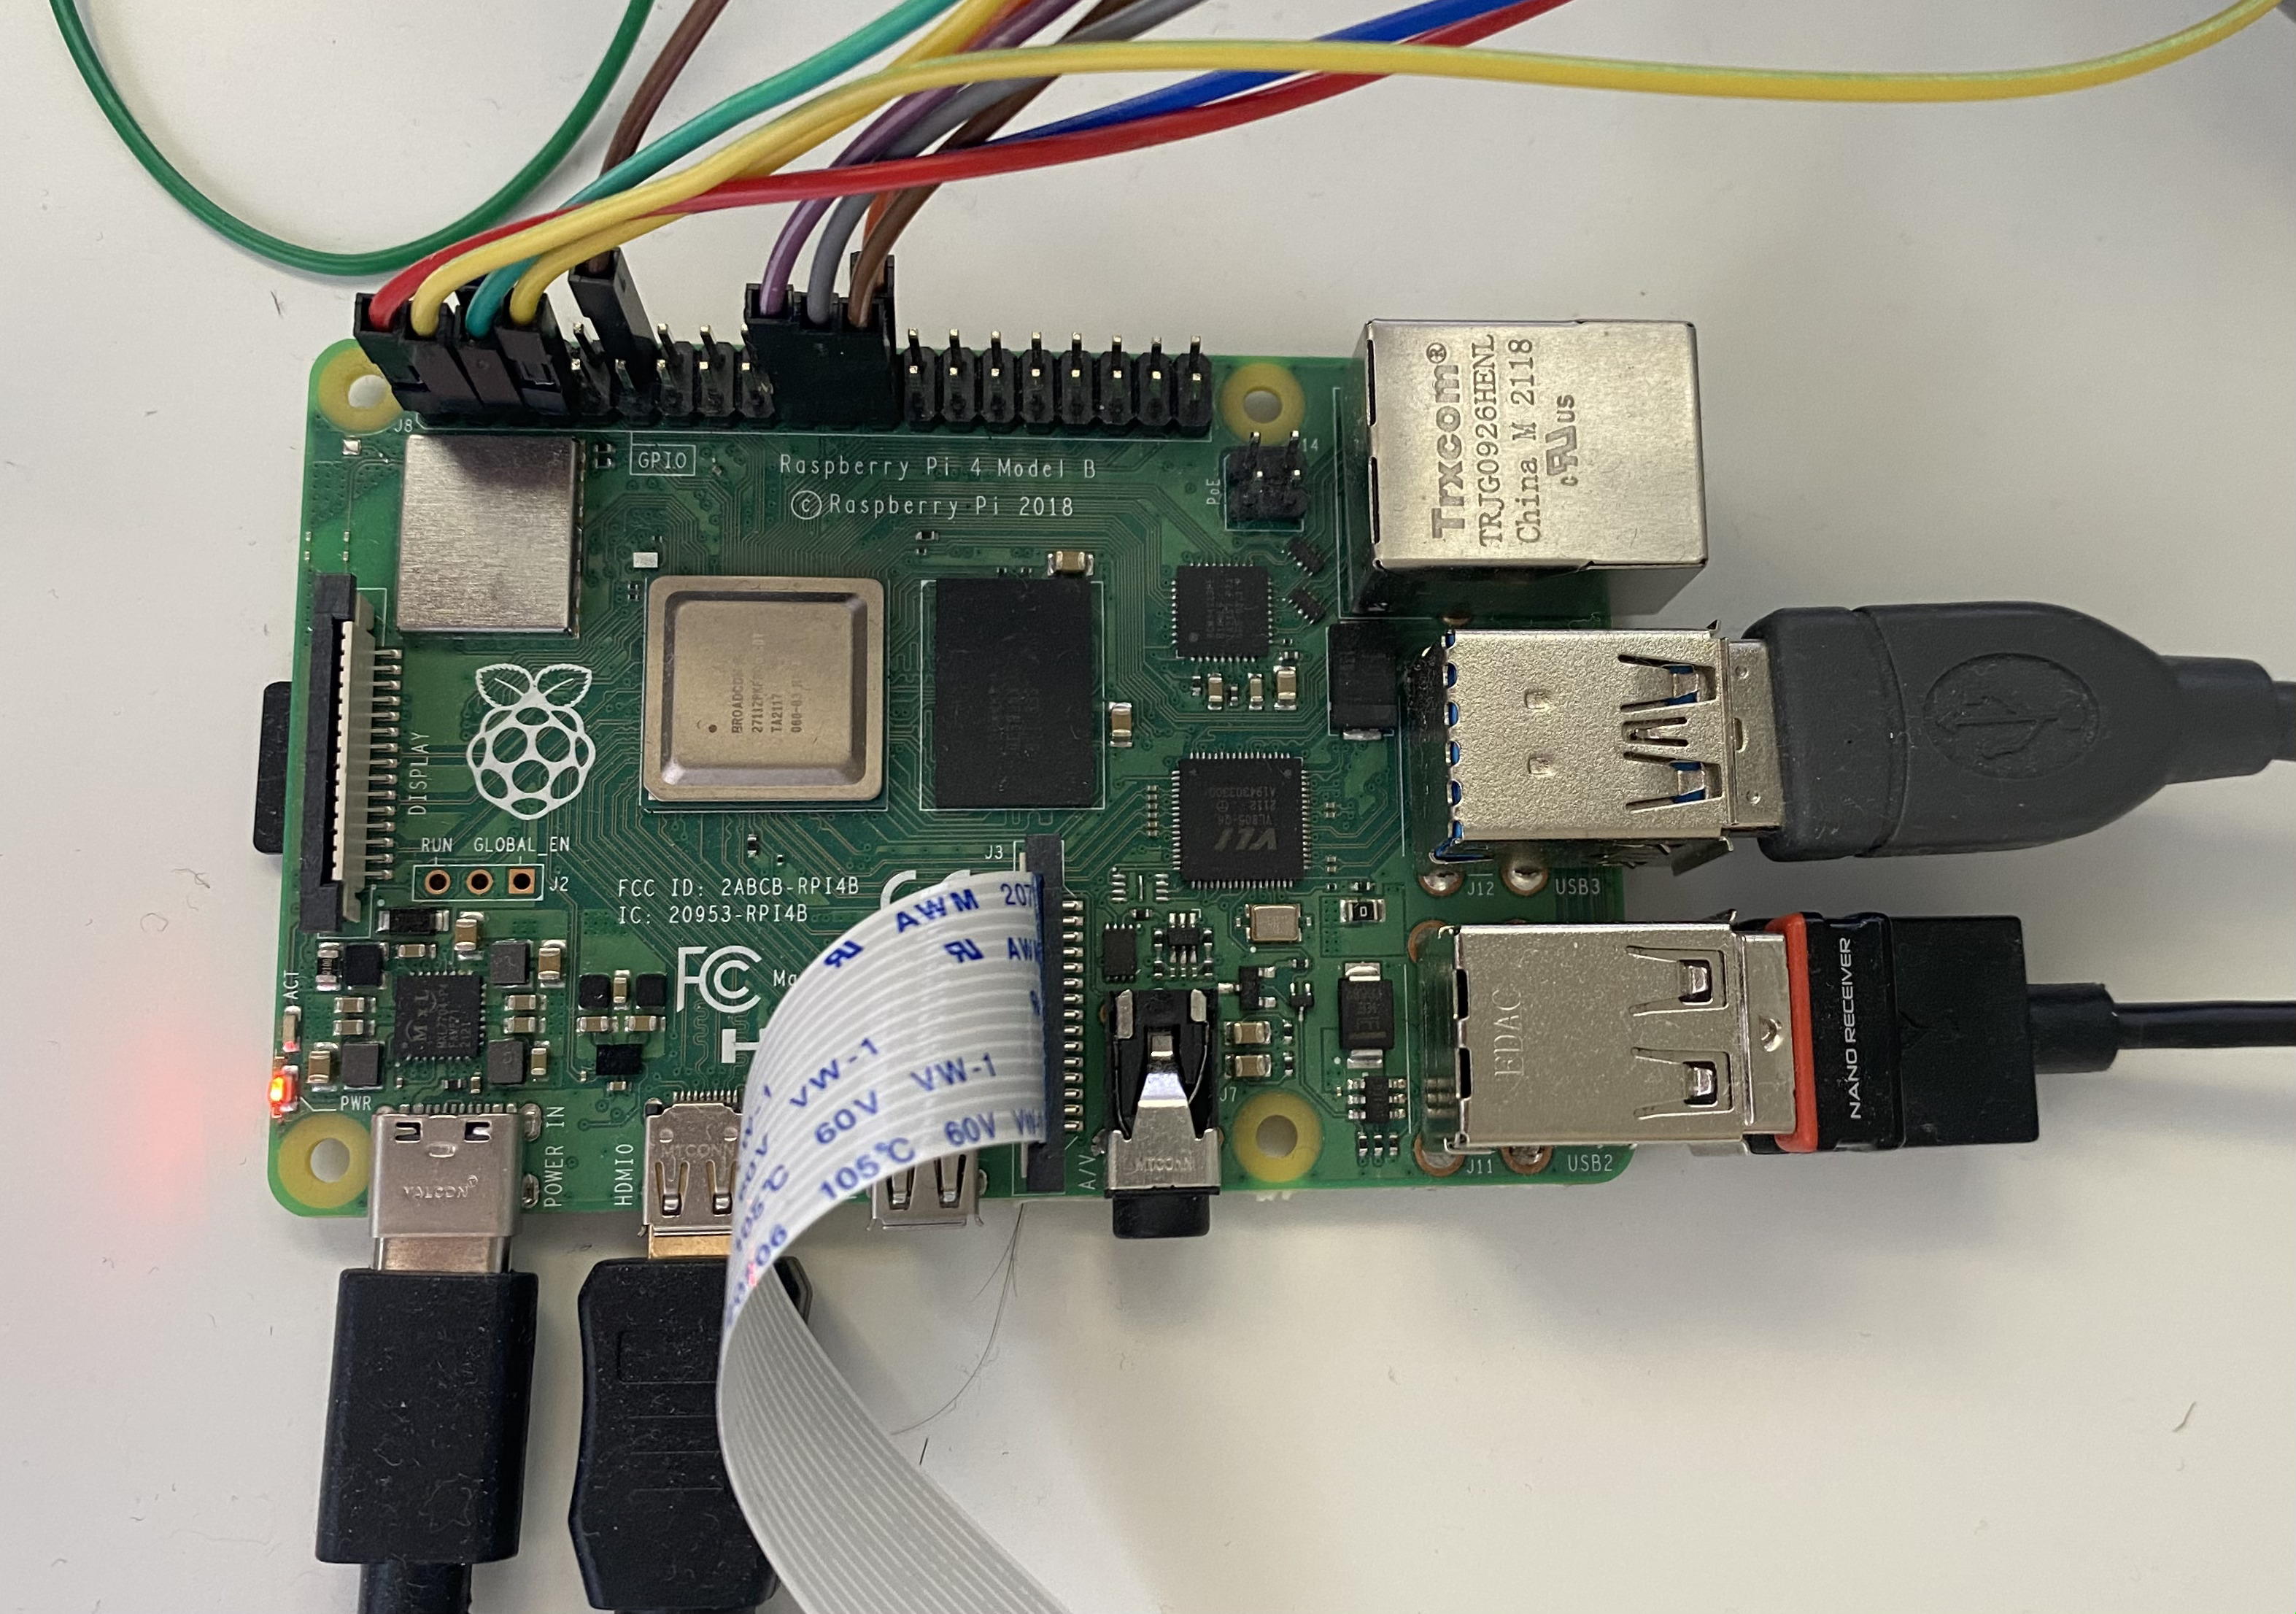
\includegraphics[width=12cm]{figs/raspberry}}\hspace{1mm}
    \subfigure[Entorno de trabajo en Raspbian.]{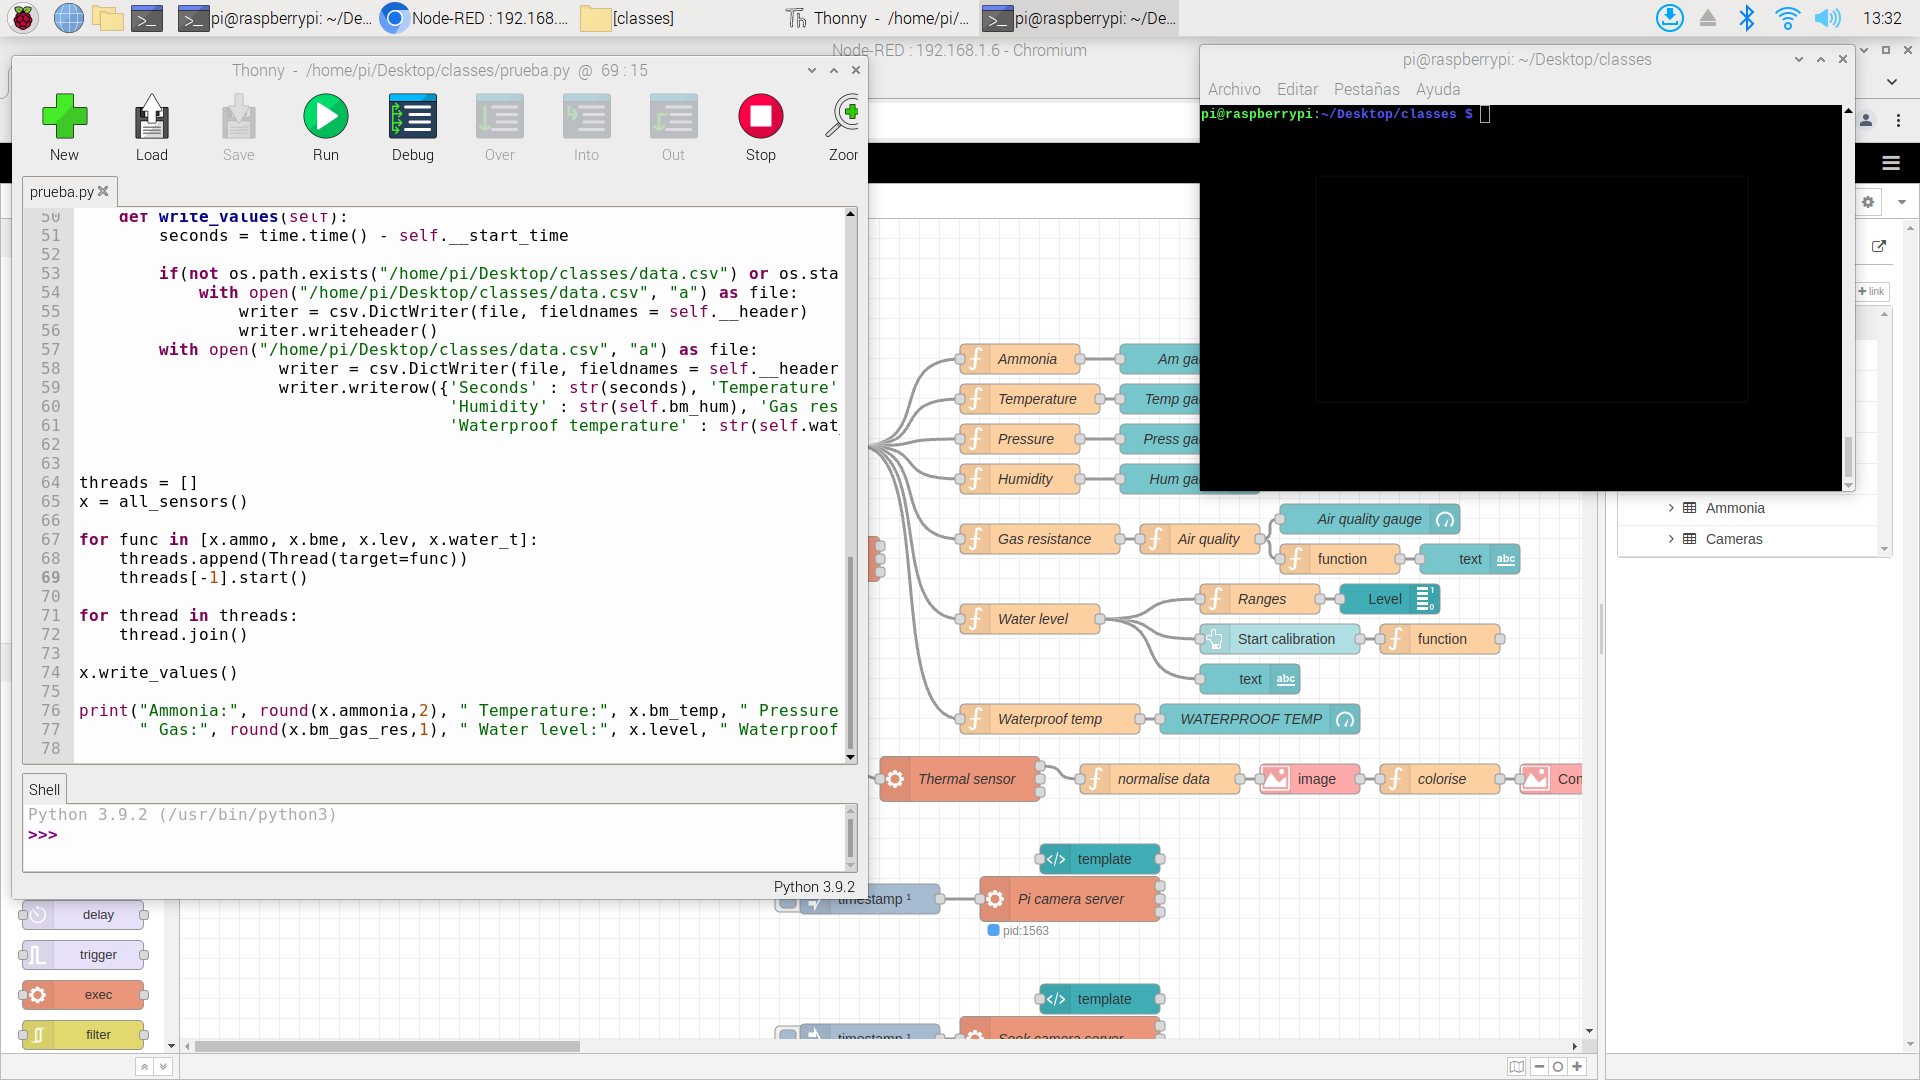
\includegraphics[width=12cm]{figs/trabajo}}
  \end{center}
\caption{Imágenes del HW y SW usados para el TFG.} \label{fig:rasp}
\end{figure}

Se han utilizado los puertos GPIO para la conexión de los distintos sensores presentados en la Sección \ref{sec:hw}. En la figura \ref{fig:esquema} se encuentran las distintas conexiones de los sensores a la Raspberry. 
\begin{figure} [h!]
  \begin{center}
    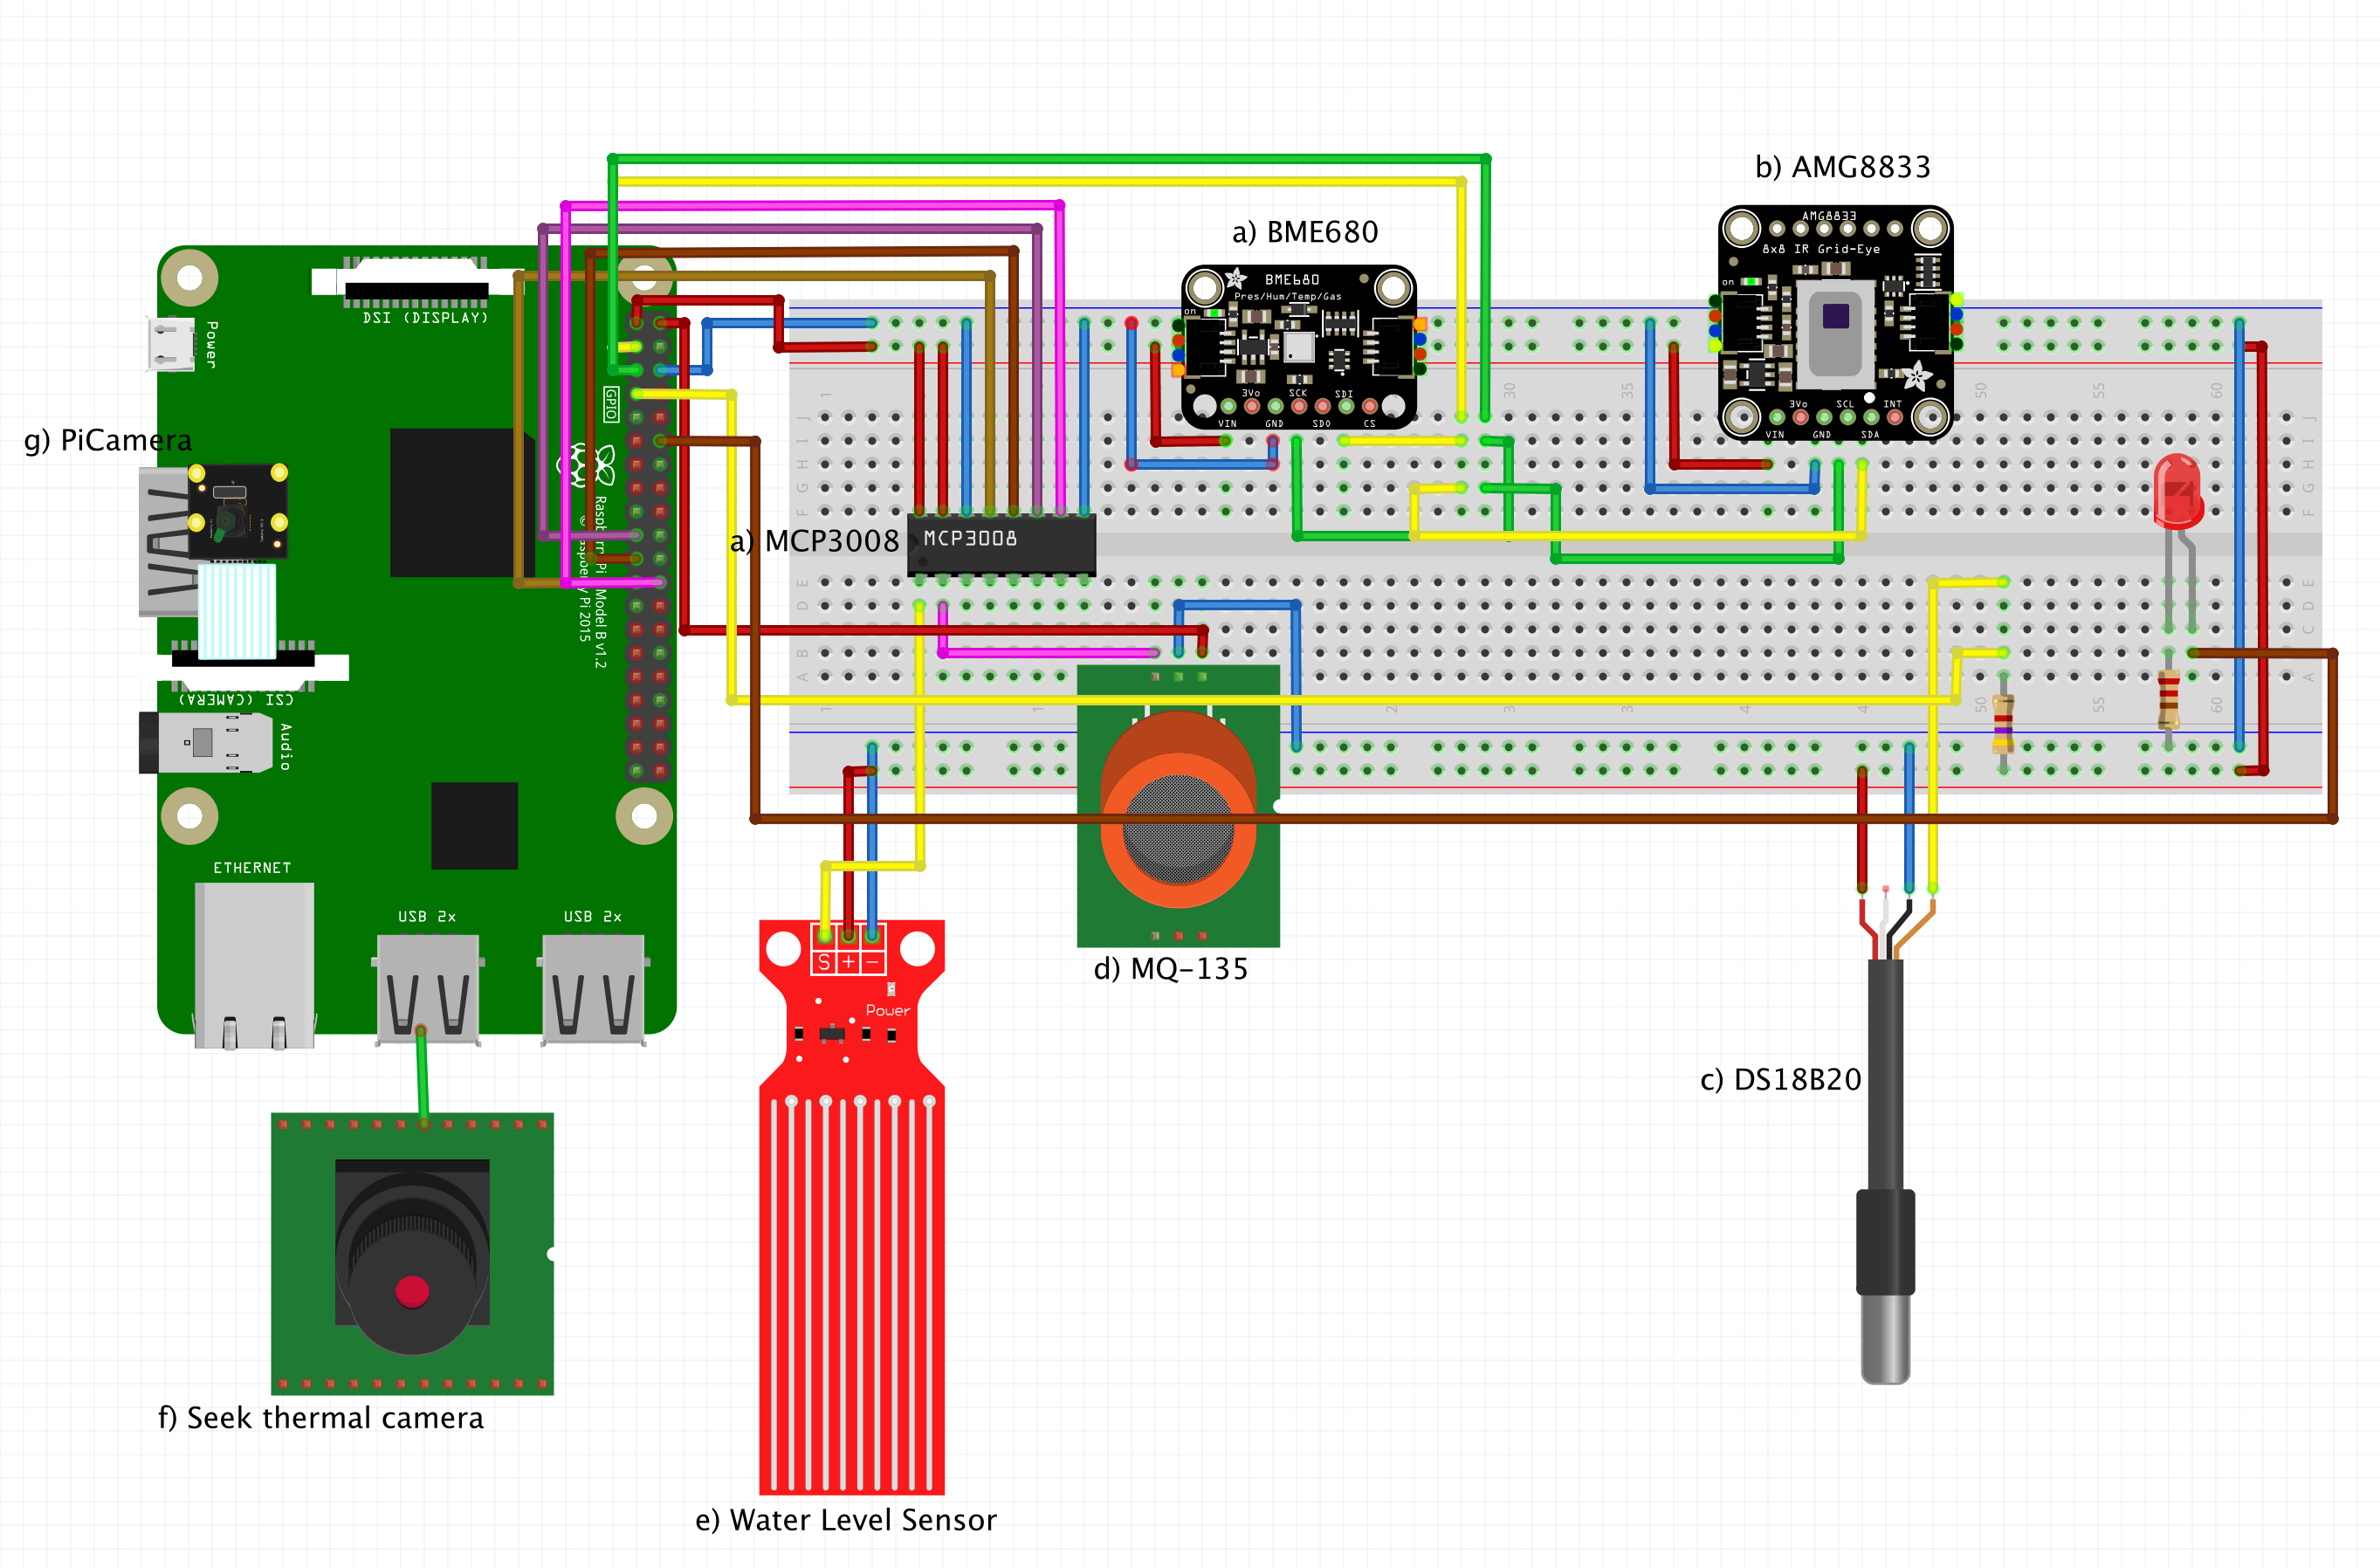
\includegraphics[width=14cm]{figs/esquema}
  \end{center}
  \caption{Esquema de conexiones.}
  \label{fig:esquema}
\end{figure}

A continuación se explican con más detalle la conexión de estos sensores:
\begin{itemize}
\item{Sensor BME680 (Figura \ref{fig:bme_of}).} Este sensor funciona con conexión I2C, que necesita dos pines, SDA y SCL para su funcionamiento. Por tanto, se ha conectado a los pines 3 y 5. También se ha conectado al pin 1 para obtener la alimentación de 3.3V que necesita y al pin 6, para evitar que se rompa el sensor.

\item{Sensor AMG8833 (Figura \ref{fig:termicos}-a).} Este sensor también funciona con conexión I2C. Por tanto su conexión es igual al sensor anterior: Conexión a los pines 3 y 5 para la conexión I2C y a los pines 1 y 6 para la alimentación y tierra, respectivamente. En la Figura \ref{fig:esquema}, la conexión a alimentación viene representada con el cable rojo, la conexión a tierra con el cable azul, la conexión I2C al pin SDA con el cable amarillo y la conexión I2C al pin SCL con el cable verde.

\item{Sensor DS18B20 (Figura \ref{fig:ds_of}).} Este sensor necesita ser conectado con una resistencia de 4.7K $\Omega$ para mantener los datos estables. Su conexión por tanto es a los pines 1 y 6 para alimentación a 3.3V y tierra, y al pin 7 para la obtención de las medidas.

\item{MQ-135 (Figura \ref{fig:mq_of}).} Este sensor necesita ser conectado a un conversor analógico a digital debido a que se deben obtener medidas analógicas. Como aparece en la Figura \ref{fig:esquema}, se ha conectado al conversor MCP3008. Además, se ha conectado a los pines 2 para la alimentación de 5V que necesita y 6 para la conexión a tierra.

\item{Sensor nivel de agua (Figura \ref{fig:nivel_of}).} Igual que el sensor anterior necesita lecturas analógicas, por lo que se ha conectado al conversor, al pin 1 para la alimentación de 3.3V y al 6 para la conexión a tierra.

\item{Seek thermal (Figura \ref{fig:termicos}-b).} Este sensor se ha conectado a través de una de las entradas USB que dispone Raspberry usando un conversor de USB a micro USB.

\item{PiCamera (Figura \ref{fig:picam_of}).} Este sensor se ha conectado en el puerto J3 que ofrece Raspberry para la conexión de su cámara. 
\end{itemize}

\begin{figure} [h!]
  \begin{center}
    \includegraphics[width=8cm]{figs/temps}
  \end{center}
  \caption{Imagen generada después de la conversión de los datos numéricos.}
  \label{fig:temps}
\end{figure}

\section{Desarrollo software}
\label{sec:dessw}
Tras diseñar la plataforma hardware, el siguiente paso es darle el soporte software. Y es que, para que este sistema funcione, es necesario crear las instrucciones y reglas a través de programas o aplicaciones, esto es, la parte software.\\

El primer, y más importante paso en cualquier desarrollo software es establecer los requisitos del sistema. Para ello, y como se ha comentado previamente, se han mantenido reuniones con el Laboratorio de Bienestar Animal de la Universidad de Alcalá de Henares, así como reuniones semanales con el tutor. De estas reuniones se ha obtenido la información necesaria para poder hacer el diseño software del sistema, que queda reflejado mediante el diagrama de casos de uso (Figura \ref{fig:casos}) y, tras un análisis de este, el diagrama de clases (Figura \ref{fig:umlet}).\\
\begin{figure} [h!]
  \begin{center}
    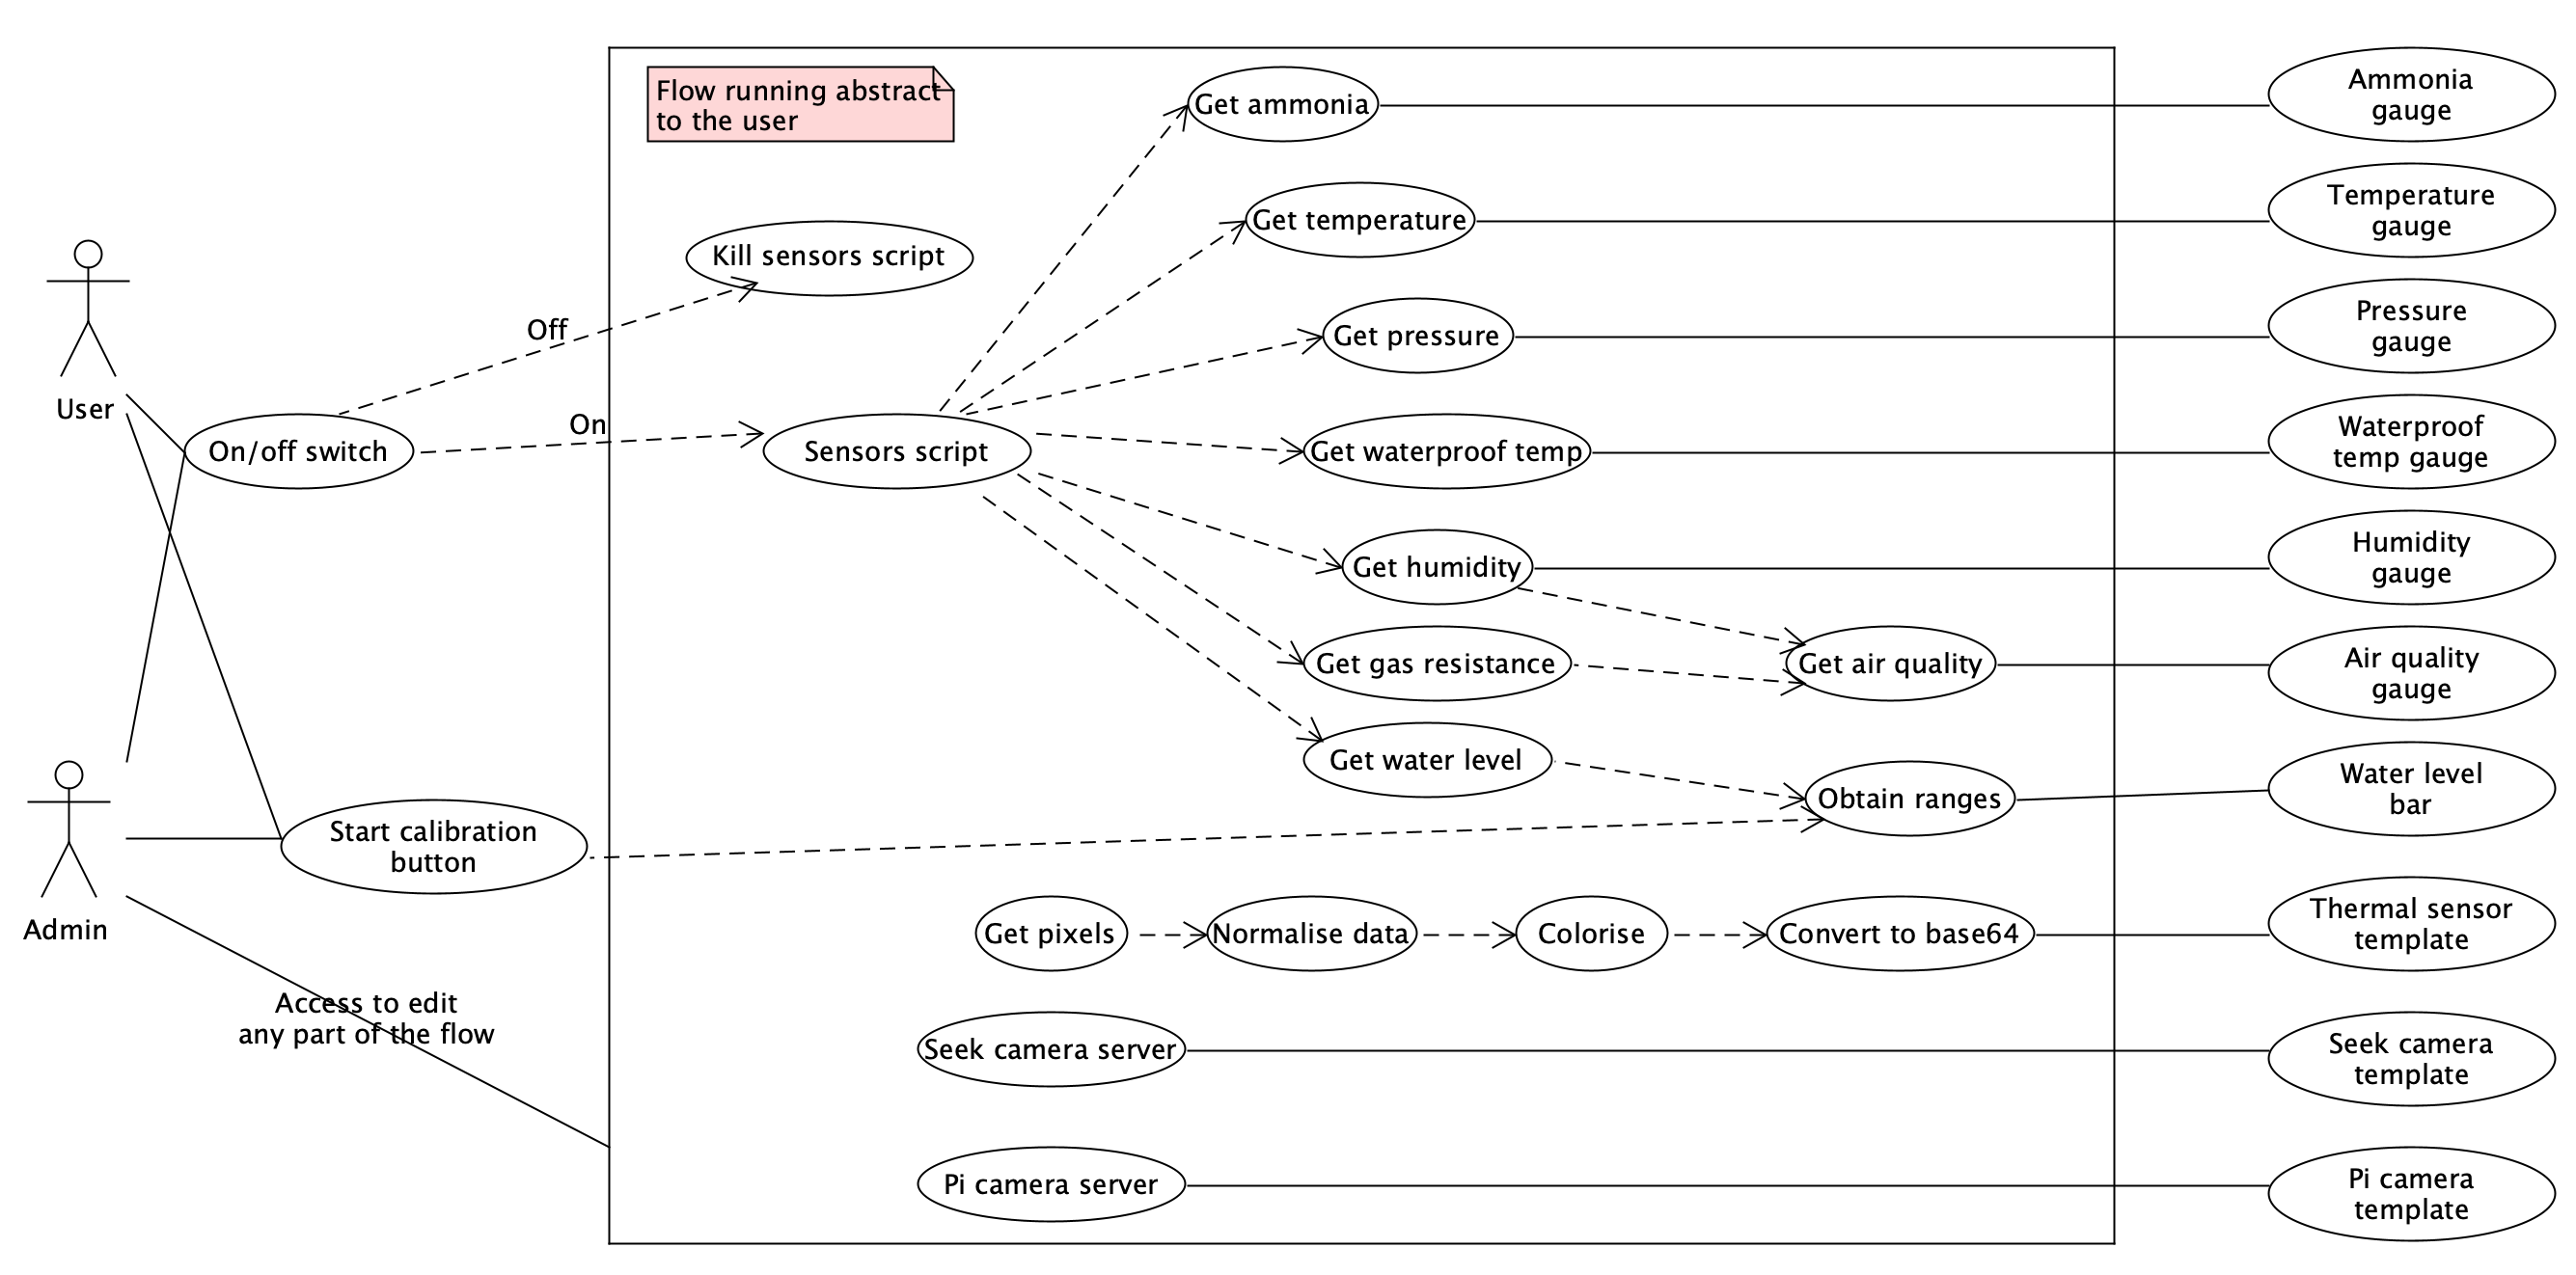
\includegraphics[width=17cm]{figs/casos}
  \end{center}
  \caption{Diagrama de casos de uso del sistema.}
  \label{fig:casos}
\end{figure}

\begin{figure} [h!]
  \begin{center}
    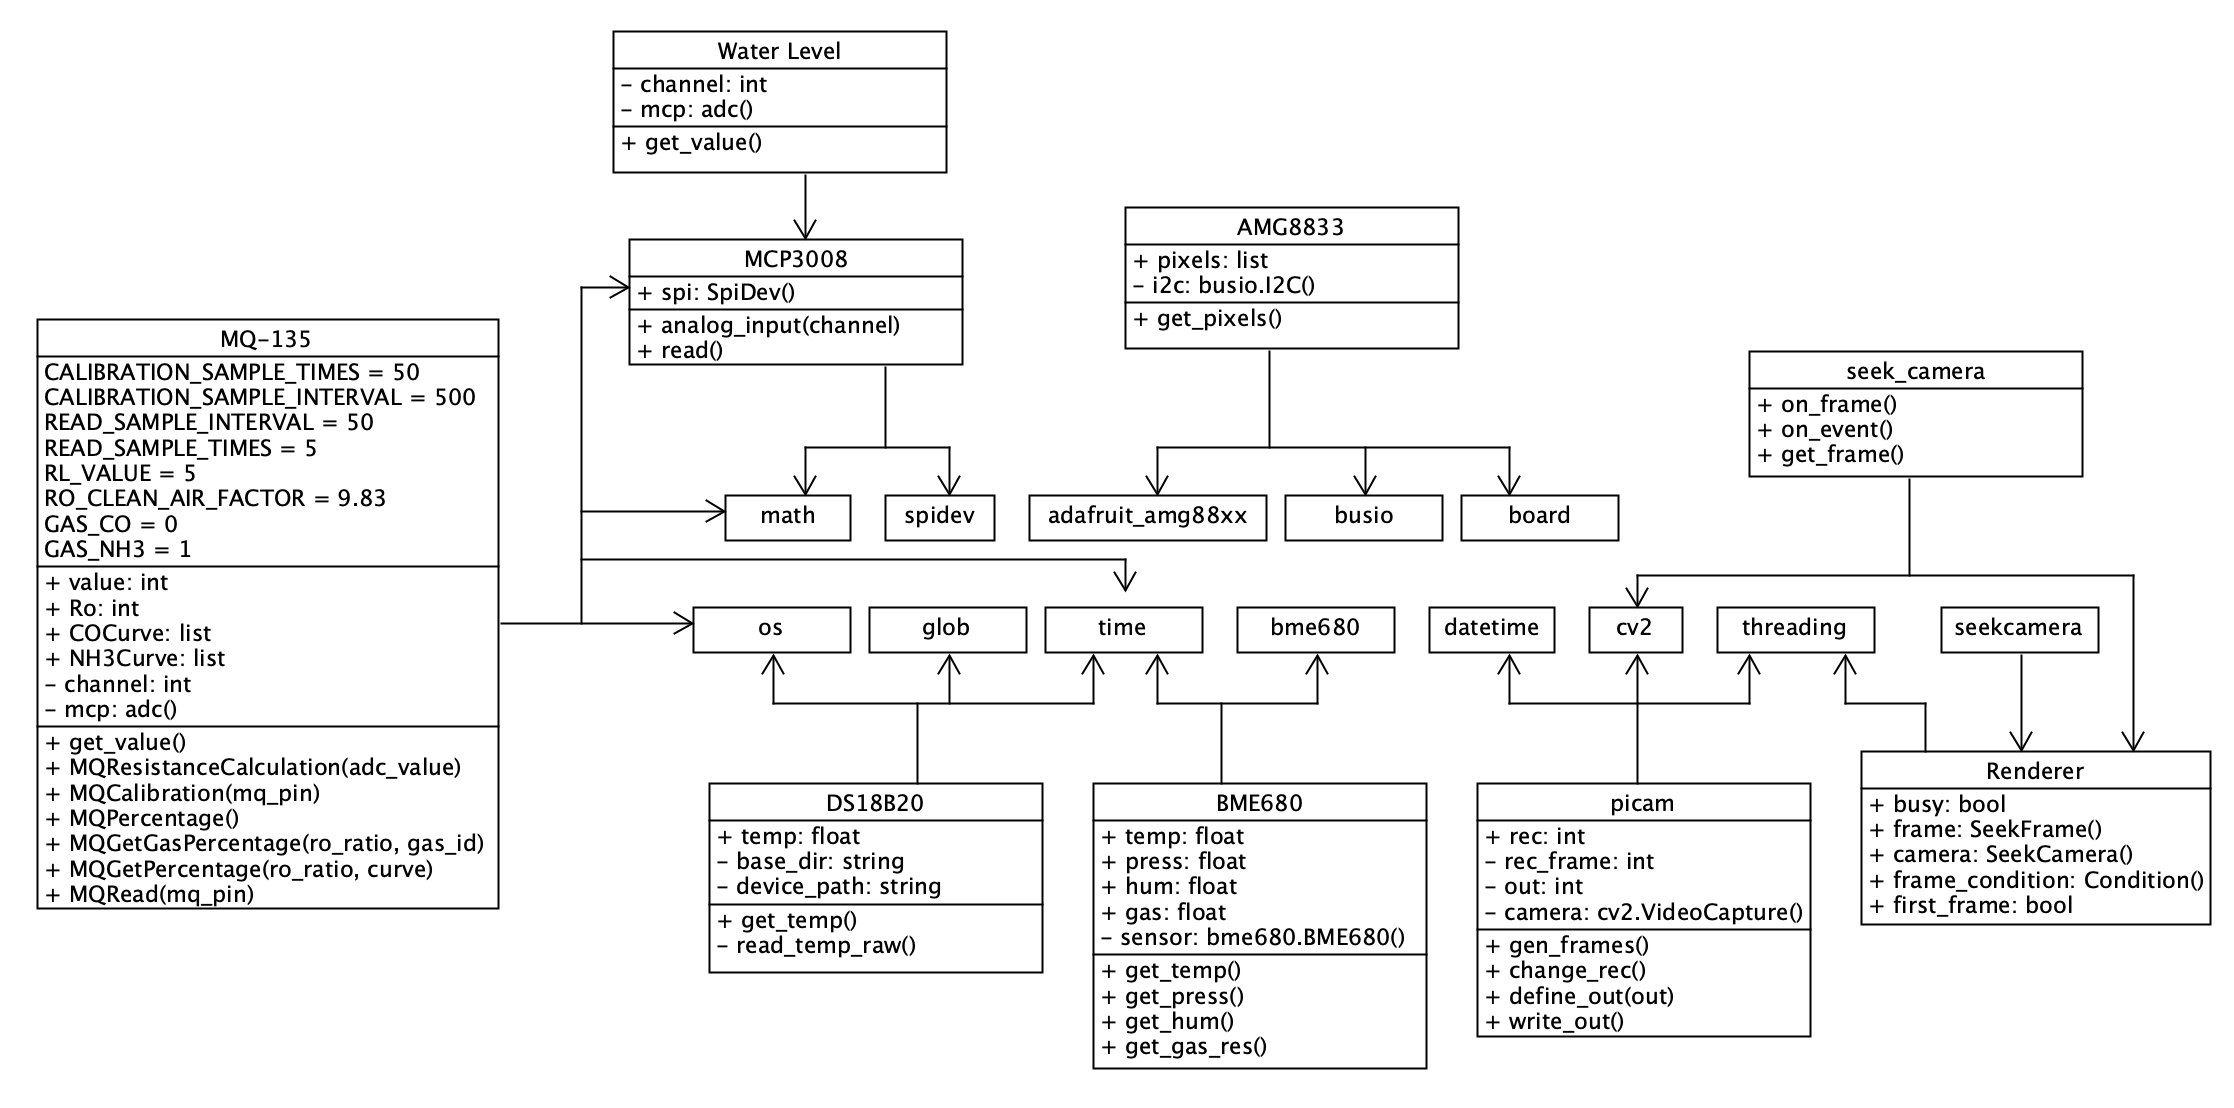
\includegraphics[width=17cm]{figs/umlet}
  \end{center}
  \caption{Diagrama de clases del sistema.}
  \label{fig:umlet}
\end{figure}

En primer lugar, ha sido necesaria la instalación de distintas librerías que dan soporte a los diferentes sensores. Tras la instalación han surgido varios problemas al intentar leer algunos sensores. Uno de los problemas encontrado en dos sensores ---los que funcionaban con conexión i2c--- ha sido que la Raspberry no los detectaba. Se puede encontrar una descripción detallada de los errores que han surgido durante la instalación de las librerías y las respectivas soluciones para hacer funcionar todos los sensores en la wiki\footnote{\url{https://github.com/jmvega/tfg-icebollada/wiki/2.February-progress}} que se ha creado para el proyecto.\\

Durante este proceso, ha habido dos sensores que se han intentado utilizar sin éxito debido a que no tienen compatibilidad con Raspberry: CCS811, que mide la calidad del aire y AM2315, que mide temperatura y humedad. Aun así, esto no ha sido un problema ya que son datos que se han podido obtener con otros sensores.\\

\subsection{Lectura sensorial con Python}
\label{sec:ficheropython}
Dado que el clinete final del sistema puede carecer de nociones avanzadas en informática, es necesario realizar diferentes cambios para ofrecer una comprensión fácil al usuario de los datos obtenidos por los sensores. Se ha utilizado el entorno Node-Red para ofrecer una interfaz amigable al usuario, de forma que este sea capaz de ver la información del estado del sistema representada a través de \textit{widgets}. Este interfaz se ha basado en el diagrama de casos de uso expuesto anteriormente en la Figura \ref{fig:casos}.\\

Para poder mostrar todos los sensores en tiempo real en Node-Red, ha sido necesario disponer de un fichero de Python que cada vez que se ejecute lea una sola vez de todos ellos. No debe leer continuamente ya que es la configuración de Node-Red la que se encarga de ello. En este fichero se procesan todos los sensores menos el AMG8833 (Figura \ref{fig:termicos}-a), la PiCam (Figura \ref{fig:picam_of}) y la cámara térmica (Figura \ref{fig:termicos}-b). Para crear este fichero se ha creado una clase por cada sensor, tal y como se estableció en el diagrama de clases (Figura \ref{fig:umlet}).\\

Este fichero de Python utiliza la librería \verb|Threads| para poder leer de manera concurrente todos los sensores, ahorrando tiempo y ganando eficacia. El Código \ref{cod:threads} muestra cómo se crea un hilo ---o thread--- por cada sensor.\\
\begin{code}[h]
\begin{lstlisting}[language=Python]
threads = []

#Lista de funciones que devuelven la lectura del sensor respectivo
for func in [x.ammo, x.bme, x.lev, x.water_t]: 
	threads.append(Thread(target=func))
	threads[-1].start()
	
for thread in threads:
	thread.join()
\end{lstlisting}
\caption[Función para crear un Thread por sensor y obtener su lectura.]{Función para crear un Thread por sensor y obtener su lectura.}
\label{cod:threads}
\end{code}

Además, este programa guarda las lecturas en un fichero CSV, por si fuese necesaria la comparación o estudio de datos a lo largo del tiempo. El fichero devuelve una cadena con la lectura de cada sensor (Código \ref{cod:salida}), para poder procesar la salida en Node-Red.\\
\begin{code}[h]
\begin{lstlisting}[language=Python]
Ammonia: 0.91 Temperature: 28.24  Pressure: 1002.1 Humidity: 52.2 Gas: 4005.9 Water level: 2 Waterproof temp: 28.312
\end{lstlisting}
\caption[Ejemplo de salida del fichero Python]{Ejemplo de salida del fichero Python}
\label{cod:salida}
\end{code}

\subsection{Creación de la interfaz de usuario}
\label{sec:IU}
Una vez creado este fichero, se ha procedido a crear la interfaz en Node-Red. Este programa funciona a través de diferentes tipos de nodos, que deben ser combinados para obtener el resultado deseado.\\

En primer lugar, a través del nodo de ejecución, se pueden ejecutar ficheros que están en la máquina local. Este nodo es el que se ha utilizado para integrar en la aplicación el fichero presentado en la Sección \ref{sec:ficheropython}. Para obtener individualmente el valor de cada sensor, se ha utilizado otro nodo ---llamado nodo función--- que permite incluir código directamente en Node-Red. Este nodo se ha utilizado para extraer de la salida del nodo ejecución el valor de interés en cada caso. Este proceso corresponde a las diferentes elipses salientes de \textit{sensors script} del diagrama de casos de uso (Figura \ref{fig:casos}). Con estos dos nodos, algunos sensores han estado listos para mostrar los valores en la interfaz de usuario (IU), por lo que solo ha sido necesario añadir el \textit{widget} más adecuado para cada caso a través del nodo pertinente. Este ha sido el caso de los sensores MQ-135 (Figura \ref{fig:mq_of}), BME680 (Figura \ref{fig:bme_of}) (en el caso de temperatura, presión y humedad) y DS18B20 (Figura \ref{fig:ds_of}).\\

En el caso de los otros sensores, han sido necesarios otros cambios para obtener el resultado adecuado:
\begin{itemize}
	\item El sensor BME680 (Figura \ref{fig:bme_of}) mide la resistencia del gas, pero se ha considerado que no es un parámetro intuitivo y no proporciona conocimiento al usuario. Por ello se ha utilizado otro nodo función que primero realiza la media de 50 lecturas de resistencia de gas y posteriormente establece la calidad del aire en función de la humedad y resistencia del aire comparándolo con la media calculada.
	
	\item Durante diferentes pruebas, se ha detectado que el sensor que mide el nivel de agua (Figura \ref{fig:nivel_of}) no es preciso a la hora de detectar la cantidad de agua presente, solamente es preciso detectando la presencia de esta. Por tanto, se ha optado por dividir en 4 rangos el nivel de agua (Figura \ref{fig:agua}), de tal manera que el usuario tenga una idea sobre la cantidad de agua presente. Aún así, el sensor no es suficientemente preciso durante la realización de diferentes pruebas y esta opción tampoco ha sido válida. Como ajuste que dota de más precisión a este sensor, se ha incorporado un botón en la IU para poder calibrar el sensor cuando el recipiente esté lleno de agua. Todo el desarrollo y las pruebas que se han llevado a cabo con este sensor pueden ser encontradas en la wiki\footnote{\url{https://github.com/jmvega/tfg-icebollada/wiki/3.March-progress}} del proyecto.
	
	\item El sensor AMG8833 (Figura \ref{fig:termicos}-a) devuelve en su lectura una matriz de 8x8 valores. Estos valores han sido convertidos a imagen ya que este sensor es una cámara térmica. Para este proceso ha sido necesario enlazar una serie de nodos hasta poder obtener la imagen más nítida, ya que la imagen obtenida originalmente ha sido una imagen de 8x8 píxeles que no alcanzaba a diferenciar objetos. De nuevo, tanto este progreso como las diferentes soluciones obtenidas se pueden encontrar en la wiki. 
\end{itemize}
\begin{figure}[h!]
  \begin{center}
    \subfigure[]{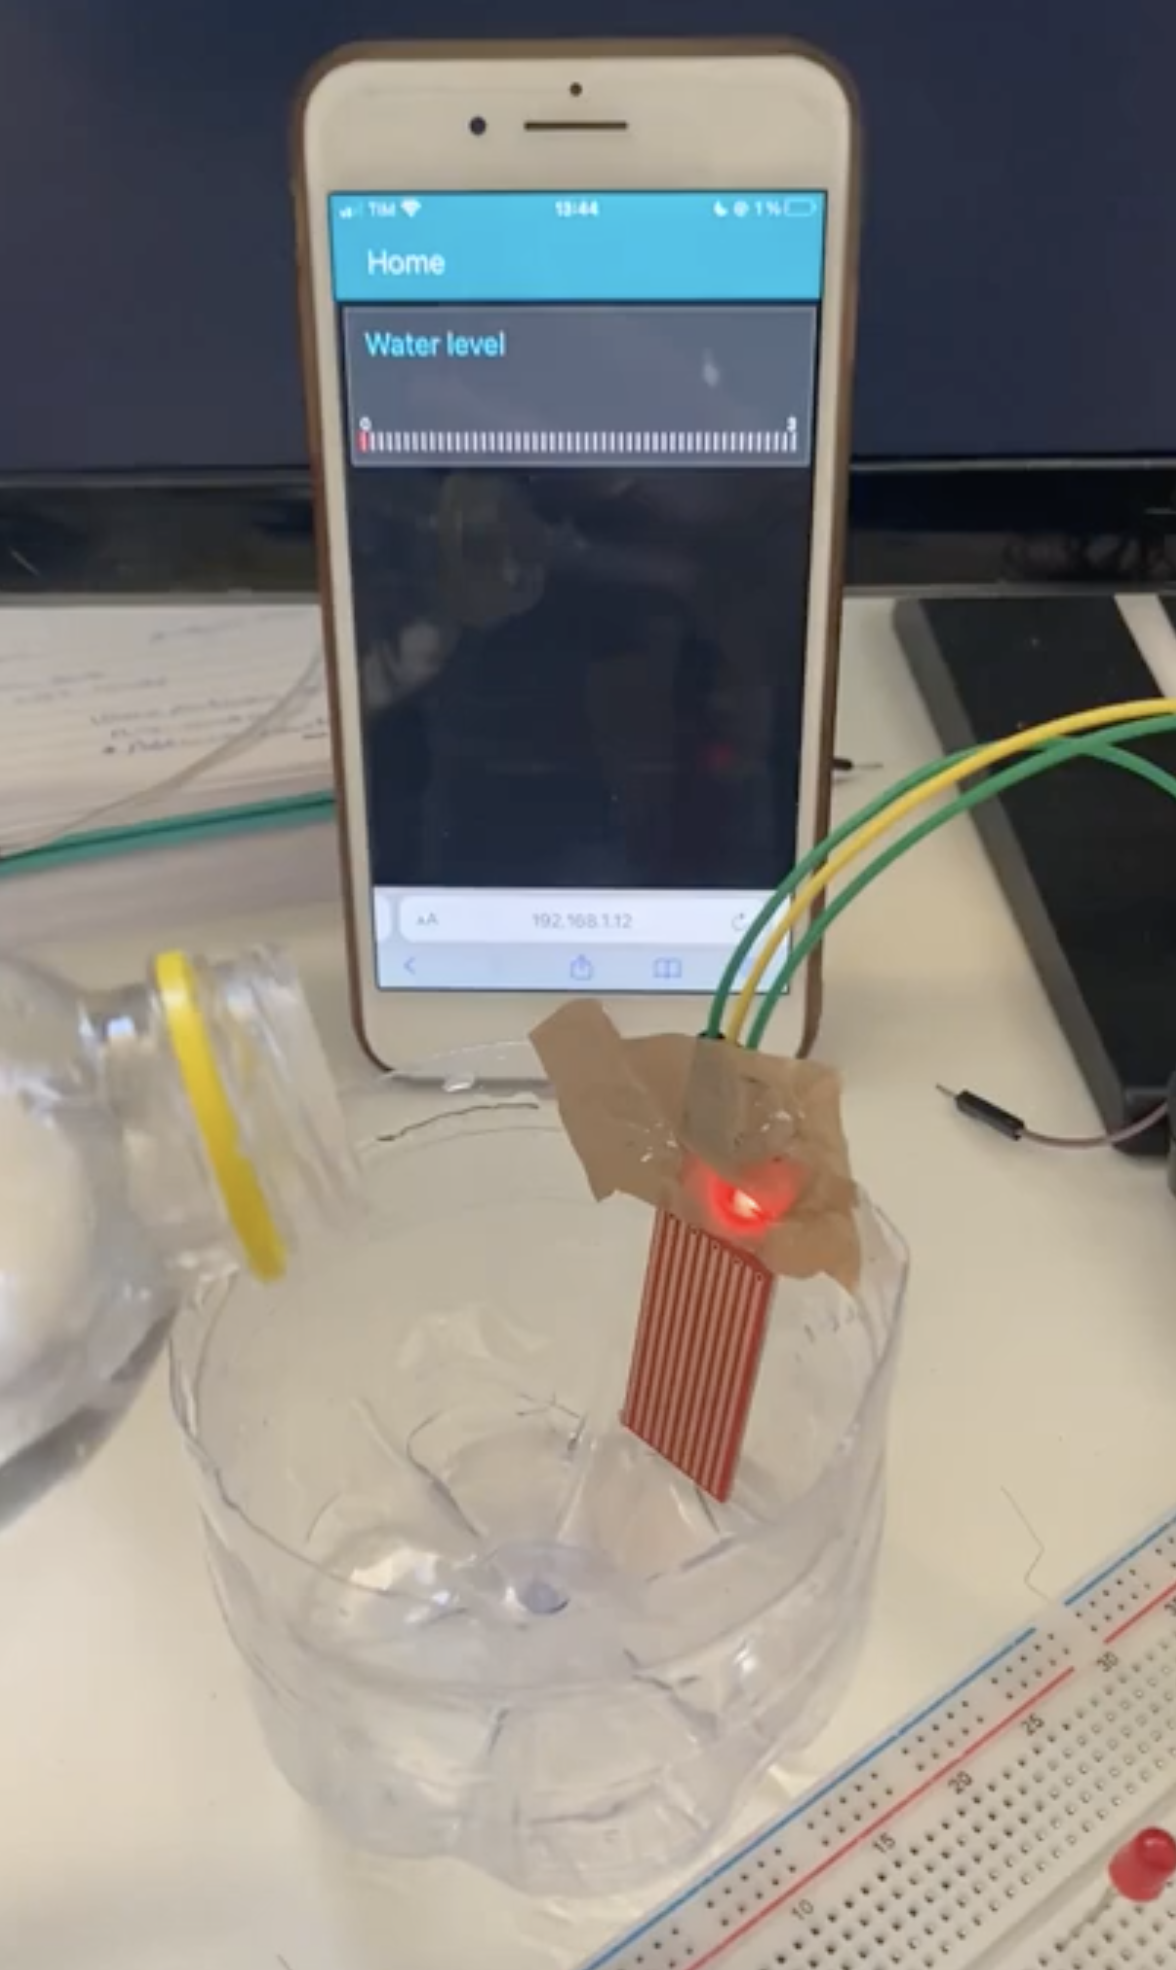
\includegraphics[width=3.4cm]{figs/agua1}}\hspace{1mm}
    \subfigure[]{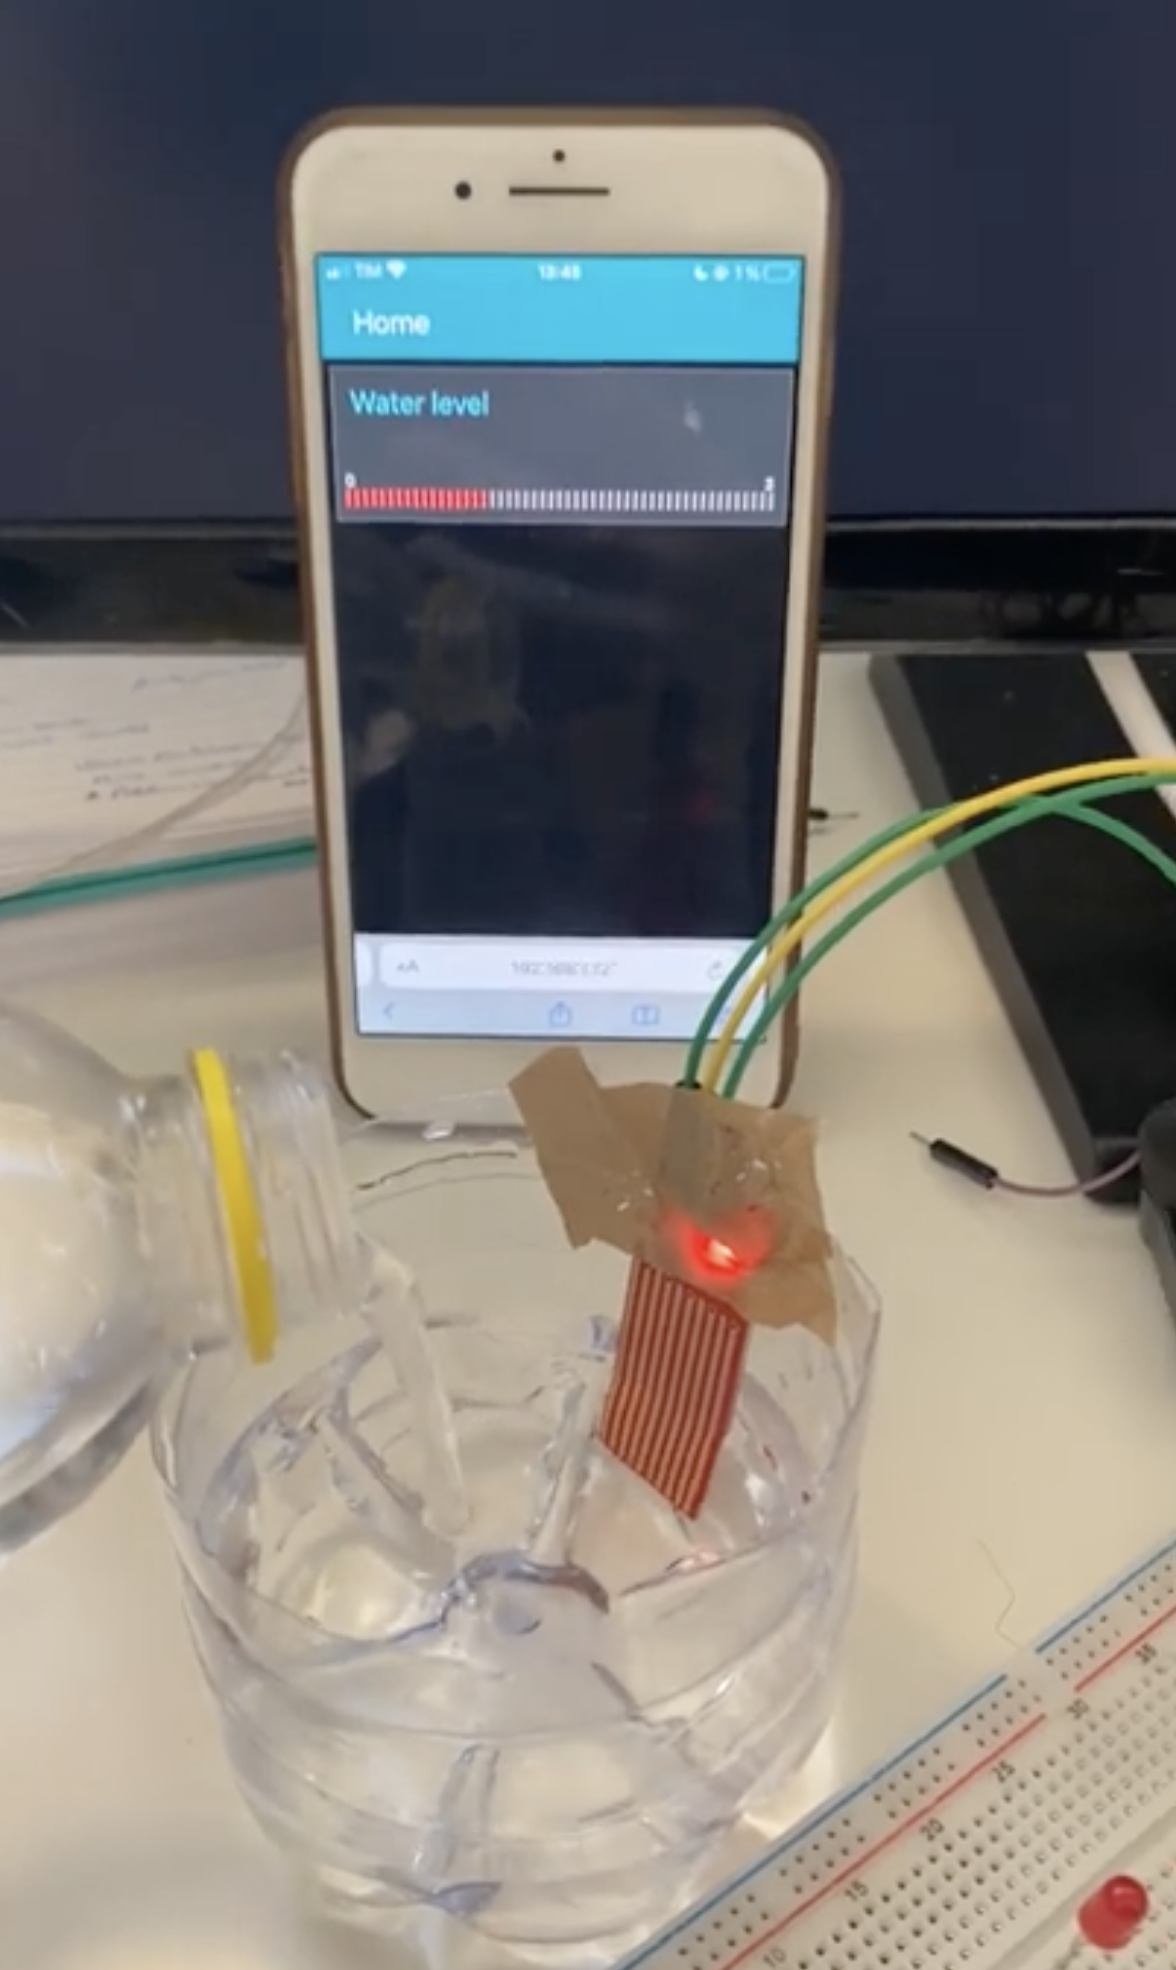
\includegraphics[width=3.4cm]{figs/agua2}}\hspace{1mm}
    \subfigure[]{\includegraphics[width=3.4cm]{figs/agua3}}\hspace{1mm}
    \subfigure[]{\includegraphics[width=3.4cm]{figs/agua4}}
  \end{center}
\caption{Proceso de indicación del nivel de agua.} \label{fig:agua}
\end{figure}

Con estos ajustes realizados, se ha obtenido parte de la IU. Para hacerla más completa se ha incorporado un interruptor de forma que el usuario puede decidir si apagarla o bien mantenerla encendida, así como un nodo que regula la repetitividad del sistema cada 3 segundos. La interfaz formada por los sensores comentados previamente se puede ver en la Figura \ref{fig:ui_nocams}.
\begin{figure} [h!]
  \begin{center}
    \includegraphics[width=16cm]{figs/ui_nocams}
  \end{center}
  \caption{IU sin los canvas correspondientes a la utilización de las cámaras.}
  \label{fig:ui_nocams}
\end{figure}

\subsection{Integración de las cámaras en la IU}
La creación de la interfaz, descrita en la Sección \ref{sec:IU}, no es completa, ya que faltan dos de los sensores que se utilizan en este trabajo: las cámaras. Para poder visualizar las cámaras desde Node-Red debe ser a través del nodo \textit{template} (plantilla), que permite visualizar una dirección web. Por tanto, ha sido necesario crear un servidor que permita visualizar las imágenes de las dos cámaras y, con ello, poder incluirlo en la IU. Para crear este servidor se ha utilizado Flask.\\

Se ha decidido crear un servidor por cada cámara. De esta manera se puede acceder solamente a una visualización o bien a las dos, según el interés del usuario. Para el funcionamiento de la cámara térmica Seek Thermal (Figura \ref{fig:termicos}-b) se ha utilizado la librería que tiene Seek, que permite su visualización a través de OpenCV. Para el funcionamiento de la PiCam (Figura \ref{fig:picam_of}) se ha utilizado OpenCV, tanto para su visualización como para la incrustación de la fecha y la hora en las imágenes (Figura \ref{fig:fechayhora}). El Código \ref{cod:fechayhora} muestra cómo se consigue.\\
\begin{figure} [h!]
  \begin{center}
    \includegraphics[width=8cm]{figs/fechayhora}
  \end{center}
  \caption{Incorporación de la fecha y hora en la visualización de la PiCam.}
  \label{fig:fechayhora}
\end{figure}

\begin{code}[h]
\begin{lstlisting}[language=Python]
ret, frame = self.__camera.read()
frame = cv2.rectangle(frame, (2,2), (275,35), (255,255,255), -1)
frame = cv2.putText(frame, str(datetime.datetime.now().replace(microsecond=0)), (10,25), cv2.FONT_HERSEY_SIMPLEX, 0.7, (0,0,0), 1, cv2.LINE_AA))
\end{lstlisting}
\caption[Código para incorporar la fecha en la esquina superior izquierda.]{Código para incorporar la fecha en la esquina superior izquierda.}
\label{cod:fechayhora}
\end{code}

Una vez obtenidas las imágenes de las cámaras desde la Raspberry, se ha incorporado al código el uso de Flask para poder crear el servidor. Es necesario disponer de dos elementos: el código para mostrar la imagen de la cámara, y una carpeta donde están las plantillas. Estas plantillas son ficheros escritos en html que muestran en el servidor la página que interesa en cada momento. La estructura que sigue un programa con Flask es la representada en el Código \ref{cod:flask}.\\
\begin{code}[h]
\begin{lstlisting}[language=Python]
from flask import *
app = Flask(__name__)

@app.route('/')
def home():
   return render_template('index.html')

if __name__ == '__main__':
   app.run(host='0.0.0.0', port=8000, debug=True)
\end{lstlisting}
\caption[Código simple que crea un servidor web en el puerto 8000 y muestra el contenido de index.html.]{Código simple que crea un servidor web y muestra el contenido de index.html.}
\label{cod:flask}
\end{code}

Después de incorporar el código del funcionamiento de cada cámara en los respectivos servidores, se ha añadido un botón para iniciar o parar la grabación del vídeo en la cámara normal. Para diferenciar cuándo se está grabando de cuándo no, se ha añadido un mensaje en pantalla indicando que se está grabando. El vídeo se guarda en la Raspberry de forma local y en formato .avi. En la Figura \ref{fig:proceso} se puede ver el proceso de registro en el servidor para acceder a la visualización de la PiCamera.\\
\begin{figure}[h!]
  \begin{center}
    \subfigure[Pantalla inicial del servidor]{\includegraphics[width=7cm]{figs/server1}}\hspace{1mm}
    \subfigure[Pantalla de registro]{\includegraphics[width=7cm]{figs/server2}}\hspace{2mm}
    \subfigure[Código de doble autenticación]{\includegraphics[width=7cm]{figs/server3}}\hspace{1mm}
    \subfigure[Escaneo de código]{\includegraphics[width=7cm]{figs/server4}}
    \subfigure[Pantalla de login]{\includegraphics[width=7cm]{figs/server6}}\hspace{2mm}
    \subfigure[Visualización de la cámara]{\includegraphics[width=7cm]{figs/server7}}
  \end{center}
\caption{Proceso de registro en el servidor de Flask de la PiCam.} \label{fig:proceso}
\end{figure}

Una vez se ha obtenido la visualización de las cámaras en la IU junto al resto de sensores, la interfaz está completada siguiendo la estructura presentada en el diagrama de casos de uso (Figura \ref{fig:casos}).


\subsection{Seguridad}
Debido a que se está trabajando en un servidor web, es importante dotar de cierta seguridad a este para que sólo las personas autorizadas puedan acceder a las imágenes. Para ello, se ha implementado el factor de doble autenticación (del inglés Two Factor Authentication, 2FA). 2FA es el proceso de autenticación donde se añade un segundo paso en el proceso de identificación frente a un servicio (por ejemplo, mediante el envío de un SMS de confirmación). En este caso, además de que un usuario introduzca su contraseña, es necesario un código que se genera cada 30 segundos y caduca pasado ese tiempo. La generación de este código se hace a través de Google Authenticator\footnote{\url{https://chrome.google.com/webstore/detail/authenticator/bhghoamapcdpbohphigoooaddinpkbai?hl=es}}. Esta extensión de Google genera los códigos (de 30 segundos de vida) a partir del escaneo de un código QR (Figura \ref{fig:proceso}-d) o por la inserción manual de un código inicial.\\

Para que estos servidores funcionen con 2FA, ha sido necesario incorporar otras librerías, así como otros módulos de Flask: Flask\_login, Flask\_bootstrap, Flask\_sqlalchemy y Flask\_wtf. Durante el desarrollo del servidor con 2FA han surgido determinados problemas, que pueden encontrarse junto a la solución en la wiki del proyecto\footnote{\url{https://github.com/jmvega/tfg-icebollada/wiki/5.May-progress}}.\\

Una vez los servidores web han funcionado, se han integrado en Node-Red a través del nodo \textit{template}. Un servidor está en el puerto 5000 y, el otro, en el 8000, para que así puedan estar ambas cámaras disponibles a la vez. Una vez añadidos, la interfaz de usuario (Figura \ref{fig:UIcompleta}) queda completa.\\
\begin{figure} [h!]
  \begin{center}
    \includegraphics[width=16cm]{figs/UIcompleta}
  \end{center}
  \caption{Visualización de la interfaz de usuario.}
  \label{fig:UIcompleta}
\end{figure}

También se ha tenido en cuenta que Node-Red funciona sobre una dirección a la que puede acceder cualquier usuario de la red sobre el puerto 1880. Por tanto, es imprescindible que sean solo los usuarios autorizados los que puedan acceder a esta plataforma, sobre todo en la parte del flujo de nodos. Así, se ha optado por dividir este acceso en dos partes. Una de ellas, la parte de administrador (Figura \ref{fig:adminlogin}), donde se encuentra el flujo de nodos y se crea toda la interfaz de usuario; únicamente un administrador debe poder acceder a esta parte, ya que es importante que una persona que no tiene conocimientos acerca de su funcionamiento no pueda realizar modificaciones. La otra parte corresponde a la interfaz de usuario (Figura \ref{fig:userlogin}); solo un usuario registrado conocedor de la contraseña puede acceder al sistema. Tanto las contraseñas de Node-Red como las de los servidores se guardan encriptadas bajo algoritmos de funciones hash en SHA256.\\ 
\begin{figure} [h!]
  \begin{center}
    \includegraphics[width=12cm]{figs/adminlogin}
  \end{center}
  \caption{Acceso al flujo de nodos en Node-Red.}
  \label{fig:adminlogin}
\end{figure}

\begin{figure}[h!]
  \begin{center}
    \subfigure[]{\includegraphics[width=60mm]{figs/phonelogin}}\hspace{2mm}
    \subfigure[]{\includegraphics[width=150mm]{figs/maclogin}}
  \end{center}
\caption{Acceso a la interfaz de usuario desde distintos dispositivos.} \label{fig:userlogin}
\end{figure}


Por otro lado, tanto los servidores de Flask como Node-Red se lanzan, por defecto, bajo una URL de HTTP (Hypertext Transfer Protocol). Por tanto, un cambio necesario ha sido añadir seguridad, de tal forma que sea HTTPS (Hypertext Transfer Protocol Secure), para impedir que otros usuarios puedan interceptar la información confidencial que se transfiere entre el cliente y los servidores web a través de Internet. Este cambio se ha realizado añadiendo certificados autofirmados creados por el autor.\\

\subsection{Autoarranque}
Recordando que este sistema está pensado para personas que no están familiarizadas con la programación o los ordenadores, se ha considerado añadir una opción que facilite el arranque del sistema.\\

Con el encendido de la Raspberry, la interfaz de usuario se lanza de forma automática ---así como los dos servidores--- y se enciende solicitando el login del usuario para acceder a la IU. Además, se ha incorporado un led verde que se ilumina cuando el sistema está listo para ser usado. El funcionamiento del autoarranque, tanto de Node-Red como de los servidores, se encuentra detallado en la wiki\footnote{\url{https://github.com/jmvega/tfg-icebollada/wiki/5.May-progress}}. El proceso de autoarranque es visible en la Figura \ref{fig:autoarranque}.
\begin{figure}[h!]
  \begin{center}
    \subfigure[Encendido de la Raspberry]{\includegraphics[width=7cm]{figs/auto1}}\hspace{1mm}
    \subfigure[]{\includegraphics[width=7.2cm]{figs/auto2}}\hspace{1mm}
    \subfigure[]{\includegraphics[width=7cm]{figs/auto3}}\hspace{1mm}
    \subfigure[Sistema listo para iniciar sesión]{\includegraphics[width=7.1cm]{figs/auto4}}
  \end{center}
\caption{Proceso de autoarranque del sistema.} \label{fig:autoarranque}
\end{figure}

\subsection{Detección de ratones mediante técnicas Deep Learning}
Finalmente, y cumpliendo con el tercer objetivo, se han desarrollado algoritmos para la detección de ratones. Para ello, en primer lugar, ha sido necesaria la creación de un dataset de ratones, debido a que no se ha encontrado ninguno cercano a los objetivos en Internet. Está formado por 354 imágenes: 275 para el proceso de entrenamiento y 79 para el de validación. El dataset creado está disponible en la plataforma Kaggle\footnote{\url{https://www.kaggle.com/datasets/isabelcebollada/datami}}.\\

Una vez se ha obtenido el dataset, se ha procedido a etiquetar estas imágenes mediante la aplicación \textit{labelImg}, para indicar los cuadros limitadores en los que se encuentran los objetos a detectar, en este caso, los ratones. Los ficheros resultantes son .txt compuestos por 5 parámetros: la clase, las coordenadas X e Y mínimas y X e Y máximas de los cuadros delimitadores.\\

Con las imágenes y las etiquetas formadas, se ha procedido al entrenamiento del modelo para la detección de ratones. Esta detección se ha realizado con YOLOv5. YOLO ofrece diferentes modelos que se adaptan a distintas características (Figura \ref{fig:tablayolo}). Se han probado cuatro modelos para la detección de ratones: YOLOv5x, YOLOv5m, YOLOv5s y YOLOv5n, siendo YOLOv5x el más lento pero más preciso y YOLOv5n el más rápido pero menos preciso. Debido a que el sistema se utiliza en Raspberry, es importante tener en cuenta que el rendimiento de la CPU es más limitado que en un ordenador normal. Se ha probado el primer modelo en un ordenador normal, donde los resultados han sido muy buenos: La visualización ha sido en tiempo real y la precisión muy buena. Sin embargo, este modelo no ha sido viable en Raspberry debido a la poca velocidad en la que se visualizaban las imágenes. Se ha probado el modelo YOLOv5m, pero el resultado ha sido una velocidad escasa en la placa. También se ha probado con YOLOv5s, donde las imágenes han ido más fluidas, aunque no a tiempo real, pero también la precisión en la detección de ratones ha disminuido. Como última prueba se ha probado con YOLOv5n. La precisión era muy peor que respecto al anterior, y la velocidad era prácticamente igual, por lo que la decisión final ha sido escoger el modelo YOLOv5s. A pesar de que se ha usado uno de los modelos más rápidos, en Raspberry el flujo de imágenes no es fluido. Debido a este motivo, la detección no es perfecta; pues hay detecciones incorrectas así como ocasiones en las que no detecta ratones (Figura \ref{fig:detec}). Todos los experimentos realizados pueden encontrarse en la wiki\footnote{\url{https://github.com/jmvega/tfg-icebollada/wiki/6.June-progress}} del proyecto.\\
\begin{figure}[h!]
  \begin{center}
    \subfigure[Detección correcta]{\includegraphics[width=7cm]{figs/correcta}}\hspace{1mm}
    \subfigure[Detección incorrecta]{\includegraphics[width=7cm]{figs/incorrecta}}\hspace{1mm}
    \subfigure[No detección incorrecta]{\includegraphics[width=7cm]{figs/nodeteccion}}\hspace{1mm}
    \subfigure[No detección correcta]{\includegraphics[width=7cm]{figs/nodeteccbien}}
  \end{center}
\caption{Detección de ratones con el modelo entrenado con YOLOv5s.} \label{fig:detec}
\end{figure}

El entrenamiento de YOLOv5 se lleva a cabo a través de un algoritmo de Deep Learning: una red neuronal convolucional. Este utiliza características ya entrenadas proporcionadas por \textit{coco128} ---un dataset muy grande ya existiente--- y aplica el nuevo dataset creado. Después del entrenamiento se obtienen métricas del modelo obtenido (Figura \ref{fig:metricas}), y se puede proceder a la prueba del modelo. En la Figura \ref{fig:precision} pueden verse la predicción de ratones en algunas de las imágenes de validación con el modelo entrenado.\\
\begin{figure}[h!]
  \begin{center}
    \includegraphics[width=12cm]{figs/metricas}
  \end{center}
\caption{Métricas del modelo entrenado para la detección de ratones.} \label{fig:metricas}
\end{figure}
\begin{figure}[h!]
  \begin{center}
    \includegraphics[width=12cm]{figs/precision}
  \end{center}
\caption{Detección de ratones con el modelo entrenado con YOLOv5.} \label{fig:precision}
\end{figure}
Finalmente, con el uso de Python y OpenCV, puede visualizarse la detección de ratones en tiempo real con la PiCamera y la Raspberry. 


\chapter{Conclusiones}
\label{cap:capitulo5}

%\begin{flushright}
%\begin{minipage}[]{10cm}
%\emph{Quizás algún fragmento de libro inspirador...}\\
%\end{minipage}\\

%Autor, \textit{Título}\\
%\end{flushright}

\vspace{1cm}
Por último, en este capítulo se presentan las conclusiones que se han obtenido con el desarrollo del presente trabajo. Se recapitulan los objetivos marcados al inicio del proyecto, el proceso que se ha llevado para cumplirlos, así como los diferentes problemas que han surgido y las soluciones tomadas para abordarlos. Además, se presentan unas posibles líneas futuras de continuación de este trabajo.\\

\section{Conclusiones}
Con el desarrollo de este trabajo se han logrado los objetivos establecidos en el Capítulo \ref{cap:capitulo2}. El objetivo principal era obtener un sistema multisensorial que fuese capaz de monitorizar los ratones de laboratorio y que, además, fuese de bajo coste. La idea era que los investigadores del Laboratorio de Bienestar e Investigación Animal de la Universidad de Alcalá de Henares tuviesen un sistema que les aportase información de las condiciones (de bienestar) en la que se encuentran los animales, y que también les facilitase el trabajo de supervisión de estos por medio de un sistema de monitorización. Todo ello se ha conseguido de forma plausible.\\

También se han conseguido los tres objetivos específicos. En primero de ellos era recoger la lectura de los sensores de forma paralela en un mismo fichero. El segundo objetivo consistía en la creación de un servidor web por cada cámara para poder visualizarlas desde distintos dispositivos y, finalmente, el tercer objetivo era la detección de ratones mediante un algoritmo de reconocimiento de objetos.\\

Con la elección de la placa Raspberry Pi para el desarrollo de este trabajo, se ha conseguido que el sistema implementado sea económicamente accesible para cualquier usuario. Esta placa de bajo coste ha permitido la conexión de distintos sensores a través de los distintos puertos que posee, como pines GPIO y puertos USB.\\

La lectura de los sensores se ha volcado a un fichero, el cual recibe la lectura concurrente de todos ellos gracias al uso de la librería \verb|Threads|. Además, este fichero genera un fichero CSV con los datos recogidos en cada momento, por si es necesario disponer de un seguimiento a lo largo del tiempo. Con este fichero, además de cumplir el primer objetivo, se ha podido iniciar la creación de la IU. Con el uso de Node-Red, estas lecturas numéricas se han adaptado a \textit{widgets} comprensibles para el usuario final.\\

Con el uso de Flask se ha conseguido el segundo objetivo. Ha permitido crear dos servidores web independientes para la visualización de las imágenes registradas por la PiCam (Figura \ref{fig:picam_of}) y la cámara térmica (Figura \ref{fig:termicos}-b). Estos servidores han sido protegidos con 2FA, requiriendo un login a través de nombre, contraseña y número de autenticación generado a través de Google Authenticator. Se han podido integrar en la IU de Node-Red junto a los \textit{widgets} de las lecturas de los sensores. De esta forma, se ha obtenido la IU completa accesible desde cualquier dispositivo conectado a la misma red que la Raspberry Pi.\\

Para la consecución del último objetivo, se ha creado un dataset de ratones con 354 imágenes. Posteriormente, se ha entrenado un modelo con el uso de YOLOv5, que ha permitido la detección de ratones a través de la PiCam.\\

Este Trabajo Fin de Grado supone un avance importante respecto a los sistemas equivalentes que se pueden encontrar en el mercado, pues lo hace accesible económicamente a cualquier laboratorio de investigación animal. Se han cumplido todos los objetivos marcados, además de añadir otras características como seguridad o accesibilidad desde distintos dispositivos, que aportan comodidad y confianza al usuario que utiliza el sistema.\\

Durante la realización del trabajo, se han obtenido conocimientos sobre distintos aspectos que no se dominaban, como la creación de un servidor web, además de la seguridad necesaria que este requiere. Además, se han aplicado muchos de los conocimientos adquiridos durante el Grado, y han surgido problemas que han requerido de esfuerzo y comprensión del tema trabajado para su solución.\\

\section{Líneas futuras}
En esta sección se comentan algunas vías que pueden permitir la continuidad de este trabajo para ofrecer funcionalidades que actualmente no tiene:
\begin{itemize}
\item Adaptación de la IU a un servidor accesible desde cualquier dispositivo. Actualmente, la IU es accesible por cualquier dispositivo que esté conectado a la misma red. Una funcionalidad útil sería poder acceder a ella desde cualquier sitio, para poder controlar el sistema en cualquier momento y desde cualquier lugar.
\item Análisis del comportamiento de los animales en las cubetas mediante técnicas de Deep Learning. Por ejemplo, realizar un control automático del tiempo que pasa cada ratón en los distintos sitios de la cubeta, o bien en qué cubeta pasan más tiempo los ratones permitirían a los investigadores poder realizar un análisis del comportamiento de los animales a través de la detección de ratones creada, y permitiendo identificar a los ratones individualmente, se podría incorporar esta idea al sistema desarrollado.
\item Creación de un Docker, para permitir la instalación del sistema a cualquier usuario. Con un Docker que instale todas las librerías y active los requisitos necesarios para el funcionamiento del sistema, cualquier usuario podría instalar y utilizar este sistema de una forma rápida y sencilla.
\end{itemize}

%\section{Corrector ortográfico}

%Una vez tengas todo, no olvides pasar el corrector ortográfico de \LaTeX a todos tus ficheros \textit{.tex}. En \texttt{Windows}, el propio editor \texttt{TeXworks} incluye el corrector. En \texttt{Linux}, usa \texttt{aspell} ejecutando el siguiente comando en tu terminal:

%\begin{verbatim}
%aspell --lang=es --mode=tex check capitulo1.tex
%\end{verbatim}


\clearpage
\thispagestyle{empty}

\printindex \nocite{*}
\appendix
\bibliographystyle{apalike} \bibliography{bibliografia}

\end{document}
